\documentclass[]{book}
\usepackage{lmodern}
\usepackage{amssymb,amsmath}
\usepackage{ifxetex,ifluatex}
\usepackage{fixltx2e} % provides \textsubscript
\ifnum 0\ifxetex 1\fi\ifluatex 1\fi=0 % if pdftex
  \usepackage[T1]{fontenc}
  \usepackage[utf8]{inputenc}
\else % if luatex or xelatex
  \ifxetex
    \usepackage{mathspec}
  \else
    \usepackage{fontspec}
  \fi
  \defaultfontfeatures{Ligatures=TeX,Scale=MatchLowercase}
\fi
% use upquote if available, for straight quotes in verbatim environments
\IfFileExists{upquote.sty}{\usepackage{upquote}}{}
% use microtype if available
\IfFileExists{microtype.sty}{%
\usepackage{microtype}
\UseMicrotypeSet[protrusion]{basicmath} % disable protrusion for tt fonts
}{}
\usepackage[margin=1in]{geometry}
\usepackage{hyperref}
\hypersetup{unicode=true,
            pdftitle={环境黑板报},
            pdfauthor={805},
            pdfborder={0 0 0},
            breaklinks=true}
\urlstyle{same}  % don't use monospace font for urls
\usepackage{natbib}
\bibliographystyle{plainnat}
\usepackage{longtable,booktabs}
\usepackage{graphicx,grffile}
\makeatletter
\def\maxwidth{\ifdim\Gin@nat@width>\linewidth\linewidth\else\Gin@nat@width\fi}
\def\maxheight{\ifdim\Gin@nat@height>\textheight\textheight\else\Gin@nat@height\fi}
\makeatother
% Scale images if necessary, so that they will not overflow the page
% margins by default, and it is still possible to overwrite the defaults
% using explicit options in \includegraphics[width, height, ...]{}
\setkeys{Gin}{width=\maxwidth,height=\maxheight,keepaspectratio}
\IfFileExists{parskip.sty}{%
\usepackage{parskip}
}{% else
\setlength{\parindent}{0pt}
\setlength{\parskip}{6pt plus 2pt minus 1pt}
}
\setlength{\emergencystretch}{3em}  % prevent overfull lines
\providecommand{\tightlist}{%
  \setlength{\itemsep}{0pt}\setlength{\parskip}{0pt}}
\setcounter{secnumdepth}{5}
% Redefines (sub)paragraphs to behave more like sections
\ifx\paragraph\undefined\else
\let\oldparagraph\paragraph
\renewcommand{\paragraph}[1]{\oldparagraph{#1}\mbox{}}
\fi
\ifx\subparagraph\undefined\else
\let\oldsubparagraph\subparagraph
\renewcommand{\subparagraph}[1]{\oldsubparagraph{#1}\mbox{}}
\fi

%%% Use protect on footnotes to avoid problems with footnotes in titles
\let\rmarkdownfootnote\footnote%
\def\footnote{\protect\rmarkdownfootnote}

%%% Change title format to be more compact
\usepackage{titling}

% Create subtitle command for use in maketitle
\newcommand{\subtitle}[1]{
  \posttitle{
    \begin{center}\large#1\end{center}
    }
}

\setlength{\droptitle}{-2em}
  \title{环境黑板报}
  \pretitle{\vspace{\droptitle}\centering\huge}
  \posttitle{\par}
  \author{805}
  \preauthor{\centering\large\emph}
  \postauthor{\par}
  \predate{\centering\large\emph}
  \postdate{\par}
  \date{2018-01-31}

\usepackage{booktabs}
\usepackage{ctex}
\setCJKmainfont{FangSong}
\setCJKmonofont{KaiTi}
\setCJKsansfont{SimHei}
\renewcommand{\chaptername}{章}

\begin{document}
\maketitle

{
\setcounter{tocdepth}{1}
\tableofcontents
}
\chapter{前言}

环境黑板报的文章存档

\begin{itemize}
\item
  研究速递(文献综述类,尖端技术介绍等)
\item
  学理观点(基础研究类、知识类科普等)
\item
  工程实践(实用技术,应用技术介绍等)
\item
  岸芷汀兰(个人感悟、工作随笔、风采展示)
\item
  朝花夕拾(文史类、游记类、书评等)
\end{itemize}

\chapter{研究速递}

\section*{十一月}
\addcontentsline{toc}{section}{十一月}

\subsection*{研究动态}
\addcontentsline{toc}{subsection}{研究动态}

本栏目旨在介绍环境科学、环境工程与生态学及相关学科近期发表的有意思的研究

\begin{itemize}
\tightlist
\item
  海洋微塑料正在成为研究热点,但密歇根大学的 Allen Burton
  却在ES\&T上发了篇 Viewpoint
  泼冷水,在他眼里,这类研究缺少风险评价,可能毫无意义
\end{itemize}

推荐人:田振宇

文献链接 \url{http://pubs.acs.org/doi/10.1021/acs.est.7b05463}

\begin{itemize}
\tightlist
\item
  谷歌正在用车载传感器检测街道级别的空气质量
\end{itemize}

推荐人:于淼

文献链接
\url{http://flowingdata.com/2017/11/08/google-maps-street-level-air-quality-using-street-view-cars-with-sensors/}

\begin{itemize}
\tightlist
\item
  城市热岛效应所引发的温度跟相对湿度变化会影响半挥发化合物的溶解度进而影响pH值,研究人员发现巴尔的摩市跟芝加哥城市跟郊区上空的pH差异在0.8与0.65,当我们讨论区域尺度的大气污染时,城乡差异的来源可能比想象的要复杂
\end{itemize}

推荐人:于淼

文献链接 \url{http://pubs.acs.org/doi/10.1021/acs.est.7b02786}

\begin{itemize}
\tightlist
\item
  科研作图是很多研究生痛苦的一个根源,然而并不是越炫酷越好,下面这个例子可以说是一个反面教材,过多的立体化、文字化与阴影化处理丢失了图片传达信息的意图,不如直接用表格
  (编自 Andrew Gelman的博客)
\end{itemize}

推荐人:于淼

链接
\url{https://www.memphisflyer.com/NewsBlog/archives/2016/08/26/report-alcohol-crashes-down-distracted-driving-accidents-up}

\subsection*{805研究简报}
\addcontentsline{toc}{subsection}{805研究简报}

本栏目旨在介绍805班同学发表的论文

\subsubsection*{菌根耐铬机理获新进展 - 伍松林}\label{---}
\addcontentsline{toc}{subsubsection}{菌根耐铬机理获新进展 - 伍松林}

做为陆地上最为广泛的微生物之一,丛枝菌根(arbuscular mycorrhiza,
AM)真菌能与绝大多数的陆地高等植物形成共生体系,帮助植物适应养分贫瘠、干旱、重金属污染等各种逆境胁迫。AM真菌在植物耐受铬污染胁迫中具有重要作用,因而在铬污染土壤生态恢复中具有极大潜在应用价值。然而AM如何促进植物耐受铬污染尚不得而知。

最近一项研究表明AM真菌在六价铬污染情况下能够上调植物根系高亲和硫酸根转运蛋白基因的表达,促进植物根系对硫的吸收。AM真菌同时系统调控了硫在植物体内的转运和代谢以抵御铬污染胁迫。硫代谢产物如半胱氨酸(cysteine,
Cys), 谷胱甘肽(glutathione, GSH), 植物络合素(phytochelatins,
PCs)等往往能够通过巯基与金属阳离子相结合,进而降低金属毒性。基于此,研究人员推断,AM根系中应有更多的铬与巯基相结合。

然而,事实并非如此,基于同步辐射光源的XAFS分析技术发现,相比较未接种根系,接种AM真菌的根系中有较少的铬与巯基相结合,相反,磷酸结合态铬在AM根系中占主导。这似乎说明,硫代谢产物在菌根耐铬中的作用并不在于络合金属铬。有趣的是,研究人员通过相关分析初步发现,这些主要硫代谢产物(Cys,
GSH, PCs)可能在缓解铬引起的植物氧化胁迫中起着重要作用。

相关文章参见:\url{https://www.sciencedirect.com/science/article/pii/S0098847217302939}

\section*{十二月}
\addcontentsline{toc}{section}{十二月}

\subsection*{研究动态}\label{-1}
\addcontentsline{toc}{subsection}{研究动态}

\begin{itemize}
\tightlist
\item
  辣木籽被国内保健行业广为吹捧,但它其实是水处理界的明星,将其混合沙子作为滤水器可以去除99\%的颗粒物与细菌
\end{itemize}

推荐人:于淼

链接:\url{http://pubs.acs.org/doi/10.1021/acs.estlett.7b00490}

\begin{itemize}
\tightlist
\item
  这篇等了很久了,USEPA对家用净水器滤芯做的嫌疑物筛选分析和非目标分析。所采用的Brita
  Filter是美国最常见的家用简易净水器,滤芯里是活性炭和阳离子交换树脂(他们应该给我广告费啊)。饮用水里有哪些污染物?看看这篇文章吧!
\end{itemize}

推荐人:田振宇

链接:\url{https://www.sciencedirect.com/science/article/pii/S026974911732691X}

\begin{itemize}
\tightlist
\item
  把汽车型号,费用,和减排目标联系起来做分析,看看什么车既便宜又环保(可是一般电动车不好修而且开起来太肉啊,well,作者是不是收了Tesla钱了
  (●′ω`●))
\end{itemize}

推荐人:田振宇

链接:\url{http://pubs.acs.org/doi/10.1021/acs.est.6b00177}

\begin{itemize}
\tightlist
\item
  毒理学研究往往考察单一污染物对单一毒性的影响,EHP上的评论文章引用了一篇双酚类污染物复合暴露的研究指出,针对多污染物与多毒性终点的研究可能给出更多毒理学信息,也需要新的方法学创新
\end{itemize}

推荐人:于淼

链接:\url{https://ehp.niehs.nih.gov/ehp2341/}
\url{https://ehp.niehs.nih.gov/ehp2325}

\begin{itemize}
\tightlist
\item
  Environmental DNA (eDNA)
  是近些年提出的新概念,指环境样品中可直接测定的非生物来源DNA,可定量分析环境多样性变化,我很好奇这是不是那些搞基因组的发现自己技术过时了就包装下输送到考古跟环境研究领域抢经费了,不过确实是个不错的指标,有希望成为研究热点
\end{itemize}

推荐人:于淼

链接:\url{http://pubs.acs.org/doi/10.1021/acs.est.7b05199}
\url{http://www.sciencedirect.com/science/article/pii/S0006320714004443}

\begin{itemize}
\tightlist
\item
  Scripps研究所一直是化学类研究的前沿阵地,脑洞也比较大,在近期提出的一套暴露组学研究流程中研究人员使用了IBM的Watson
  AI系统来学习文献中的分子并评价暴露组学筛选出的分子,这是要让多少人丢饭碗啊
\end{itemize}

推荐人:于淼

链接:\url{http://pubs.acs.org/doi/full/10.1021/acs.analchem.7b02759}

\begin{itemize}
\tightlist
\item
  ``赏金科学家''召集令!!!美国农垦总局出价十万美金征集根除水体中斑马贻贝的方案,欢迎物种入侵相关研究组来美捞金,毕竟一个方案就是两个面上的钱,截止日期二月底
\end{itemize}

推荐人:于淼

链接:\url{https://www.innocentive.com/ar/workspace/challengeDetail?challenge=9933880}

\begin{itemize}
\tightlist
\item
  来自中国的研究组测了下海盐、湖盐和井盐中的塑料纤维,发现海盐里微塑料明显多于井盐,这个视角比较独特,直接跟食品挂钩了,不过依然缺少风险评价
\end{itemize}

推荐人:于淼

链接:\url{http://pubs.acs.org/doi/10.1021/acs.est.5b03163}

\begin{itemize}
\tightlist
\item
  这个有点像淼哥之前推荐的 Environmental DNA (eDNA)
  那个,不同的是研究者着眼于抗生素抗性基因(antibiotic resistance genes,
  ARG,
  也就是耐药超级细菌所需要的基因)。在污水处理过程中细胞相关的ARG能被较为高效地清除,但是游离的胞外ARG去除效率较低,可能是耐药基因的一个重要来源
\end{itemize}

推荐人:田振宇

链接:\url{http://pubs.acs.org/doi/10.1021/acs.est.7b04283}

\begin{itemize}
\tightlist
\item
  原来以为原生动物除了难杀灭和能引起奇怪的病之外就没啥意义。然而最近EAWAG的一项研究发现,活性污泥中的原生动物能够通过电荷吸附的作用去除污水中的胺类。
\end{itemize}

推荐人:田振宇

链接:\url{http://pubs.acs.org/doi/10.1021/acs.est.7b03556}

\begin{itemize}
\tightlist
\item
  五大湖的藻华会影响类似海盐气溶胶的淡水湖气溶胶,单颗粒质谱技术或气溶胶质谱技术有助于我们研究这一特定环境过程,这类概念很不错,但落地还是需要未知物鉴定的数据分析技术,不然还是pca游戏
\end{itemize}

推荐人:于淼

链接:\url{http://pubs.acs.org/doi/10.1021/acs.est.7b03609}

\begin{itemize}
\tightlist
\item
  拿NHANES数据集发ES\&T不新鲜,但搞个10年前的ANN算法来溯源就有点过分了,这种题目放到数据类MOOCs上当作业可能都是送分题,而且数据质量也太差了,0.3\%到0.5\%的灵敏度还不如随机噪音,没有验证集结果根本就是瞎猜
\end{itemize}

推荐人:于淼

链接:\url{http://pubs.acs.org/doi/10.1021/acs.est.7b05128}

\subsection*{805研究简报}\label{-1}
\addcontentsline{toc}{subsection}{805研究简报}

本栏目旨在介绍805班同学发表的论文

\subsubsection*{氮杂环芳烃环境过程研究新进展 - 田振宇}\label{---}
\addcontentsline{toc}{subsubsection}{氮杂环芳烃环境过程研究新进展 -
田振宇}

氮杂环芳烃(azaarenes)是多环芳烃(PAHs)的氮取代类似物。这类污染物常伴随多环芳烃同时出现在污染场地中,但是由于分析方法的限制,目前对于它们的浓度和环境行为了解十分有限。特别是已知具有较强毒性的高分子量(4-5环)氮杂环芳烃,在各种环境介质的信息都比较缺乏。现有研究大多集中于低分子量(2-3环)的少数几个同类物。换句话说,这类污染物中最危险的东西,我们了解的最少,需要填补这一信息上的空白。

基于高分辨质谱(HRMS)和质量亏损过滤(mass defect
filtering),本研究将一种非目标分析方法应用于四个不同污染场地的土壤样品,检测出8个系列共232个同类物。其中四环和五环的氮杂环芳烃被大量检出,种类和浓度都较高。对比污染场地中污染物的分布,可见风化程度高的土壤中四环和五环氮杂环芳烃比例更高。已知有毒且有致癌性的的benzo{[}c{]}acridine和dibenzo{[}a,h{]}acridine被检出,并且发现它们具有较多的同分异构体。
从本研究可以得出的主要结论是:

\begin{itemize}
\item
  由于以往的研究忽略了氮杂环芳烃的多样性,它们在污染土壤的毒性中起到的作用很可能被低估;
\item
  对于土壤中氮杂环芳烃的研究,应更多集中于以往较少关注的高分子量同类物,因为它们的浓度较高且具有持久性。
\end{itemize}

链接:\url{http://pubs.acs.org/doi/abs/10.1021/acs.est.7b03319}
(其实窝是810班的)

\section*{一月}
\addcontentsline{toc}{section}{一月}

\subsection*{研究动态}\label{-2}
\addcontentsline{toc}{subsection}{研究动态}

\begin{itemize}
\tightlist
\item
  ES\&T Letter 的执行主编是一个特别喜欢写 editorial
  的教授,哪怕一期就三四篇,在 Letter 的 IF
  没有超过正刊后,主编大人自己定义了一个 Author Impact
  Factor(AIF),用过去两年发表数除以2,然后又定义了 L 因子(用 AIF
  除以发表期刊的平均 IF
  ),不得不说这个指标就比较难刷了,有一点他说的非常在理,期刊要以发表的工作为荣,而不是反过来。
\end{itemize}

推荐人:于淼

链接:\url{http://pubs.acs.org/doi/10.1021/acs.estlett.7b00546}

\begin{itemize}
\tightlist
\item
  用高通量metagenomics
  测室内空气中的病毒核酸,采样的地方是12个大学宿舍。宿主多样性很高,而且病毒群落组成可能反映与房间居住者的关联。
\end{itemize}

推荐人:田振宇

链接:\url{http://pubs.acs.org/doi/10.1021/acs.est.7b04203}

\begin{itemize}
\tightlist
\item
  考虑停留时间,室内空气污染其实比室外影响要大,清华大学的一个研究组考察了中式烹饪过程中室内污染的影响因素,结果发现烹饪方式对大多数污染物影响最严重,基本趋势是炒菜\textgreater{}油炸\textgreater{}蒸煮,如果开了排气扇,大多数污染物浓度都能下降一半。
\end{itemize}

推荐人:于淼

链接:\url{http://pubs.acs.org/doi/10.1021/acs.est.7b05600}

\begin{itemize}
\tightlist
\item
  左旋葡聚糖经常被用来作为生物质燃烧的标志污染物进行溯源,然而最近的研究发现燃煤也可以生成左旋葡聚糖,这导致我们可能高估了北京的细颗粒物中生物质燃烧的贡献,特别是有燃煤行为的地区
\end{itemize}

推荐人:于淼

链接:\url{http://pubs.acs.org/doi/10.1021/acs.est.7b05858}

\begin{itemize}
\tightlist
\item
  关于精子质量和大气颗粒物之间关联的流行病学研究。结论比较有意思,说
  PM10 (以及与 PM2.5的差)
  与精子质量有负相关性,而不是PM2.5。但是大气颗粒物的数据来自区域性的监测和调查问卷,感觉不是很靠谱。
\end{itemize}

推荐人:田振宇

链接:\url{http://pubs.acs.org/doi/10.1021/acs.est.7b05206}

\begin{itemize}
\tightlist
\item
  光化学反应能在道路尘土中产生单线态氧。大气气相反应和水体光化学反应中的单线态氧并不稀奇,考虑到颗粒物本身就带有各种污染物,这个发现还是有点意思。和持久自由基有无关联?是否会影响stormwater
  中的污染物?可以问出一系列的问题了。
\end{itemize}

推荐人:田振宇

链接:\url{http://pubs.acs.org/doi/10.1021/acs.estlett.7b00533}

\begin{itemize}
\tightlist
\item
  欧盟在2018年又加入了7种严控污染物,有三种含镉物质,另外得克隆也进入名单了,阻燃剂从
  PBDEs
  开始,几乎就是沿着替代品路线一路禁下去,核心问题在于卤代物天然具有遇热释放卤原子猝灭火焰的特性,替代物都是沿着这个常温稳定,高温分解的思路开发,而这个思路几乎对应持久性有机污染物的特性,这个猫捉老鼠的游戏需要新技术作为搅局者来打破循环。
\end{itemize}

推荐人:于淼

链接:\url{https://echa.europa.eu/candidate-list-table}

\begin{itemize}
\tightlist
\item
  数据分析方法是长久以来被忽视的研究方向,伴随数据时代的崛起,越来越多的数据人才正在流入传统科研领域掘金,环境学科更是价值洼地,这篇
  EHP 的文章是基于 stan 构建的一个贝叶斯在线分析工具,从 stan
  角度看就是一个本科生课后作业水平,但 EHP
  在环境领域什么份量相信大家都心里有数。总之,不学习新知就会被抛弃,这是学术圈的铁律。
\end{itemize}

推荐人:于淼

链接:\url{https://ehp.niehs.nih.gov/ehp1289/}

\chapter{学理研究}

\section{混沌的冬日}

\subsection{序}

1962年,美国海洋生物学家 Rachel Carson
出版了《寂静的春天》,这本书展示了农药污染下没有虫鸣的春天。在其影响下公众开始关注环境污染问题并开启了环境科学研究的序幕。然而,国内公众对于环境污染的关注也许并不用等到春天。近几年,每每国庆刚过,雾霾就会几次三番的席卷全国,呈现出混沌的冬日。

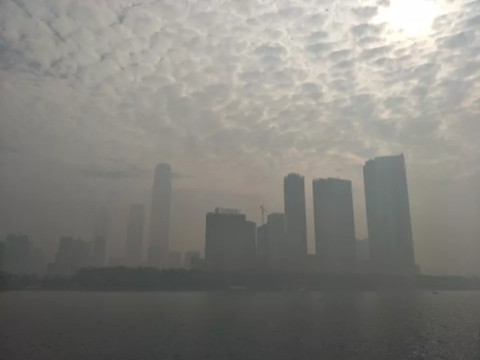
\includegraphics[width=6.67in]{images/cw1}

有人说发展的问题会在发展中解决,例如发达国家也经历过类似的阶段,但伴随产业转型与法规调控,污染问题都会自然而然地消亡;又有人说虽然城市会被雾霾笼罩,但从统计数据上看居民平均寿命其实比所谓田园风光的乡村更长;还有人说大气污染相比土壤、水还有固废污染都不算严重,只是可见度更高(也就是能见度低)\ldots{}\ldots{}的确,雾霾这个现象背后有着错综复杂的社会经济影响,从不同的角度去看会发现不一样的东西。多一个角度看问题并不会让你过的更好,但至少更明白些。

下面我将给出一些非技术与法规调控的视角,希望对读者理解雾霾以及其他一些环境污染问题能有帮助。

\subsection{研究增长的极限}

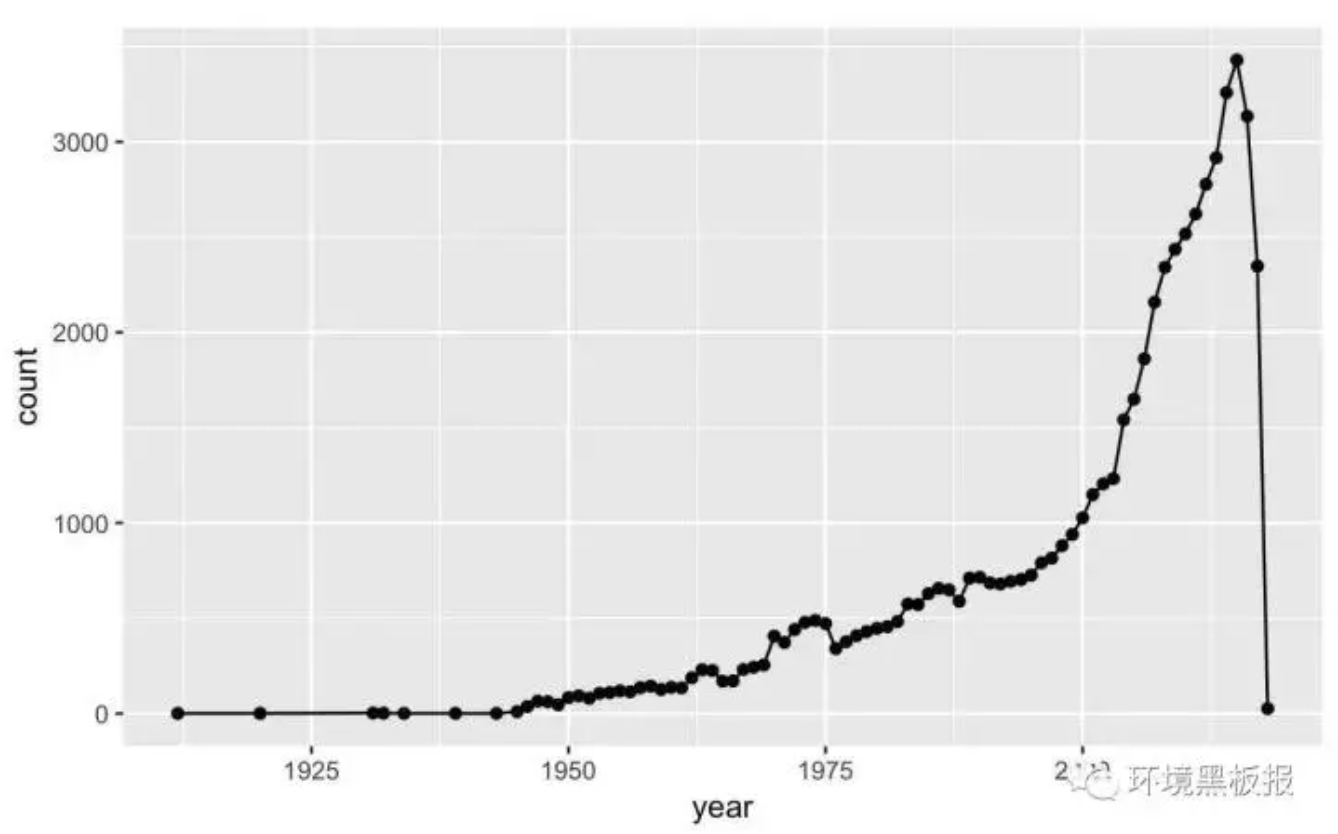
\includegraphics[width=6.67in]{images/cw2}

上图是生物资讯数据库 Pubmed 上用颗粒物(particulate
matter)作为关键词得到的论文数量,一百年来可以说是持续增长,特别是21世纪以来增长尤为迅猛。但需要注意的是到2015年达到了峰值(3429),16年已经明显下降(3134),今年还有两个月(2348),但不出意外也不会超过16年。至于为什么会有少量18年文献(26),这是学术界硬通货论文的通货膨胀,透支未来可以说是现代社会最伟大也最危险的发明,学术界亦然。也就是说,对于颗粒物的研究兴趣实际已经在降低了。

这个现象可能有点反直觉,因为近几年大气环境污染的公众关注度非常高,经费投放也很可观,但学术界却降低了学术交流频次。无独有偶,使用传统研究热点例如汞、铬、二恶英、基因组、纳米颗粒去进行检索,都会发现研究在2014-2015年间出现了峰值。但同时如果去看一些新兴研究例如3D打印,颗粒物中的细颗粒物(fine
particulate
matter),则增长还是非常迅速的(下图是以细颗粒物为关键词的文献发表状况)。

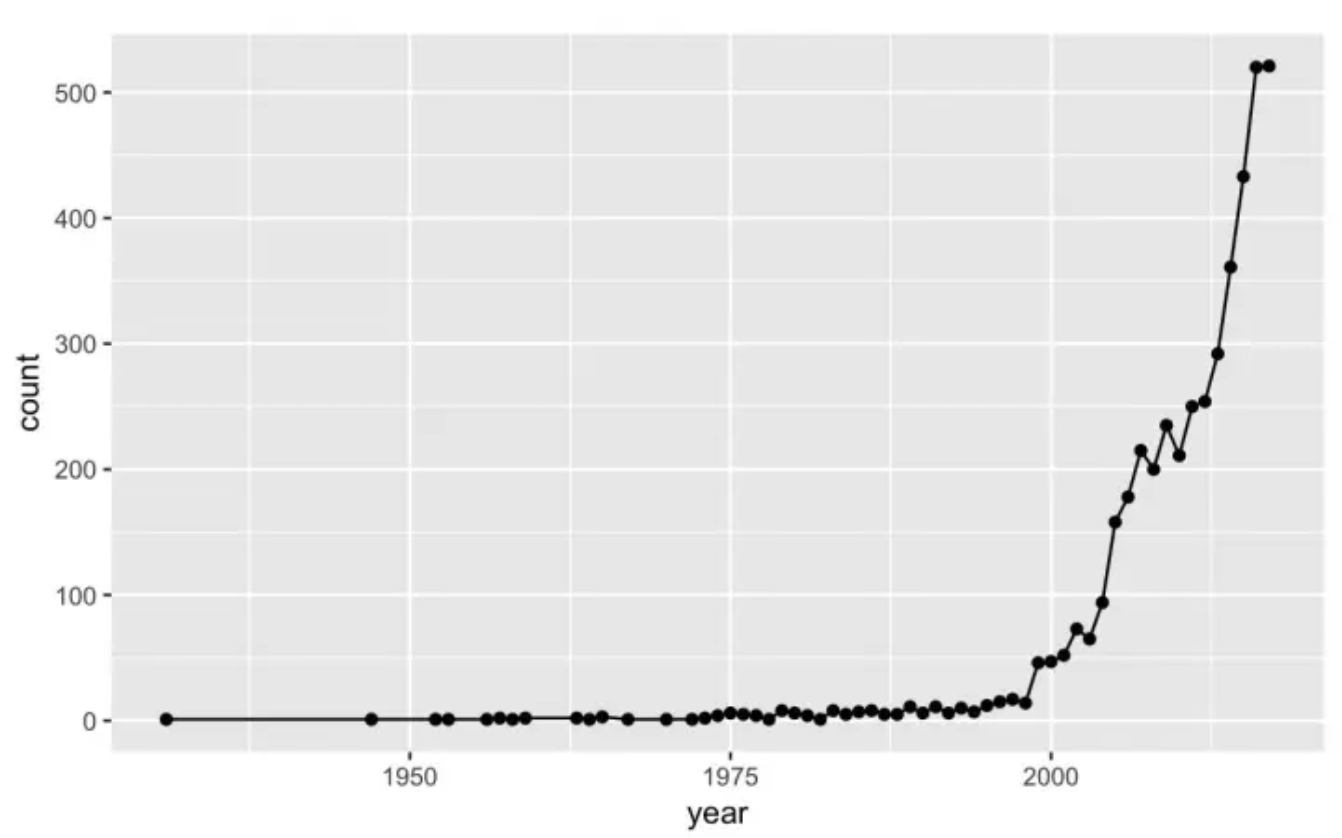
\includegraphics[width=6.67in]{images/cw3}

如果把学术界所有人的研究精力看成是总量稳定的,那么论文数可以看成精力的指标,对于包括大气颗粒物在内的很多环境研究课题而言,学术界正在把蛋糕切给更新的技术与概念。同样是进行雾霾研究,如果你从事微米尺度研究,而学术界却更加认可纳米尺度的研究,那么你的文章就很难发表,然后就是经费紧张,如此循环;进而使得新概念也不断变成老概念。

就颗粒物研究而言,目前学术圈总体关注度已经在下降,但分支中却有上升的。那么可想而知,学科内存在激烈竞争,并不是所有的颗粒物研究方向都是热点。而且还可以预期的是少数研究方向的异军突起会吸收更多学科内的研究资源,很多优秀的研究人员可能一开始选错了研究方向,最终的结局就是转行。研究的增长极限是客观存在的,所以如果你在这个年代打算去找专家咨询,最好去问上升期的新人,因为很多概念从出现到流行不到三五年,有经验的专家反而可能因为有学科内竞争关系而给出带有其自己都意识不到的感情色彩的论断。

\subsection{有原罪的雾霾}

如果某天PM2.5爆表,然后你又恰好感觉到嗓子不舒服,那么很自然你会认为这是雾霾的锅。这符合情理,但不一定符合事实,雾霾跟健康是有联系的,但跟健康有联系的可不仅仅是雾霾。即使仅仅考虑大气污染,颗粒物也只是能够产生爆表AQI的一个因素,其余的例如工业主导的硫酸型烟雾或汽车尾气主导的光化学烟雾都会影响健康,都能让嗓子不舒服,此时你会把原因归到哪里?

进一步讲,环境因素也只是影响健康的一个方面,遗传也起作用。假如你在雾霾天听到一个有气管炎家族病史的患者在咳嗽,你会认为是环境影响还是遗传作用?而根据最近Science的一份研究,即便你排除掉环境因素与遗传因素,仅仅是新陈代谢过程中DNA的复制次数就可解释癌症的发病率的66\%,而这个过程根本就无法用先天后天因素来解释,就是个生长问题。

在中国,雾霾是有原罪的,它实际承载了社会转型期人们的一部分焦虑。如果其对健康的总影响是十,那么其中真实作用可能也就二三,替遗传和其他污染物背了三四的锅,还有三四则可以说是心因性的。今年柳叶刀上一篇文献就提到,中国PM1跟PM2.5大概贡献了医院急诊的4.47\%与5.05\%。这种研究有两个问题,第一,即使排除了意外导致的急诊(例如车祸),就诊行为本身就会受天气影响;此外就是
type M
型错误(效应数量级错误),也就是说这个效应是真实的,但是影响不一定大。

这其实是目前环境研究的一个通病,找一组病人和一组正常人(有的连这个也省了)采集样本,然后一把测定几百上千种污染物(这个现在技术上是没问题的),然后算相关系数,这种情况随机你都可以发现几个的,而这样做出的发现有个通病,那就是效应通常不大,很难重现。一个小而真实的效应或许有学术价值,但舆论一放大就会产生公众心理焦虑,而心理状态又会影响生理状态,这类影响可能并不比真实影响小。

雾霾是有原罪的,但被过度聚焦了,由此产生的焦虑与恐慌本身也会产生健康影响。如果公众可以更好理解科学研究现状与其中的问题,这并不能客观降低空气污染的健康影响,但在实际意义上却可能减轻雾霾的心因性副作用。

\subsection{万金油的幻象}

不知道从什么时候开始,万金油的心态重新出现了。以前如果我告诉你有一种方法可以让你永远远离雾霾危险,你肯定说我瞎扯。好,现在我换一种说法,在人工智能+区块链+可穿戴设备+大数据的实时监控下,我可以给你一副智能眼镜,上面会实时反应你现在的风险指数,如果指数超过80\%,那么你就应该进入室内。逻辑上来说,如果你按照超过指标就躲到室内,那么这个风险永远不会变成100\%,也就是说,这跟我刚才说的永远远离雾霾危险实质等同,但是这样的产品你多半不会觉得是瞎扯,甚至会愿意付高价购买,这又是为什么?

万金油思维从来都没远离过我们,只是从熟悉的名词变成了看似专业的术语。人们有一种看起来很理性但又很荒谬的行为:乐观而盲目地相信着未知的科技。雾霾来了,那就买个最好的空气净化器;外面看不见了,那就来个3M口罩;嗓子不舒服了,那就去搞点清肺的保健品。其实很多人都知道这些科技可能还不成熟,但只要花钱了就有种事情完结可以甩锅的想法。真实的情况往往是越是大家关注的事物,就越有人去贩卖这种包装过的万金油,你买到的更多只是一个确定性的心态。


\includegraphics[width=6.67in]{images/cw4}

在这个分工细致的现代社会里,绝大多数的服务业出售的都是经过专业化包装的确定性,用来抵消分工后一颗颗螺丝钉无法感知全局的焦虑。雾霾就是个全局问题,涉及很多不同专业的知识,当个体被复杂性搞晕时,最简单的方法就是掏出一把钞票买个心安理得。即使问题不能在当前根本解决,但生活总要继续,或许这就是万金油思维在进化上的意义。在雾霾这种大IP下,科学家、政府、骗子、掮客、投机商你方唱罢我登场,过分认真你就输了。

\subsection{混沌的冬日}\label{-1}

回溯千年,宋代诗人陆游在《秋霁》中提到:``驱除云雾极知难'',除了难在技术与法规,雾霾也是直指人心的。

看看窗外,凛冬将至


\includegraphics[width=6.67in]{images/cw5}

作者:yufree 编辑:栟

\section{幻化残生}

幻化残生,也就是环境、化学、材料跟生物这四大学科的近似谐音,都属于实验比例比较高的专业。这些专业的研究生生存现状都------并不乐观。

\subsection{现状}

首先,这四个学科属于建立在脑力劳动之上的体力劳动。例如前处理、过柱、表征、养细胞、涂板子、野外采样等等,流程性非常强,到时间点上不论节假日还是凌晨饭点都得待命;但有时又会发现这些工作找个本科生带上两天也能做出来。一个尴尬的事实是,实验学科一个重要研究方向就是取代人工操作实现流程自动化与便携化,当实验简单到轻轻一按时,研究生训练得到的技能瞬间贬值,更尴尬的是实现这个过程需要的背景知识是物理、机械跟电子工程而不是幻化残生,掌握某项实验技能短期可以使你取得不错的成果,但长期看几乎一定会过时。

其次,特别拼先进仪器/技术,进而导致平台建设重于人才培养。今年这个技术能发顶刊,明年就可能被取代了;有些特殊资源例如光源没有背景想约个机时难得要命,但如果不进行一些高开支实验可能编辑就直接拒稿;而先进仪器装备的价格往往奇高,所以从经济角度,这四个学科都属于很烧钱的。那么这里的尴尬就是,你的才能可能受限于仪器平台;而从研究机构角度看,投资仪器显然比投资人才培养在初期更有效果,而人才培养初期其实也就是仪器操作。这个没啥办法,现在很多科学问题的回答其实早就脱离了理论导向阶段,而是我有一个问题想回答,但目前技术回答不了,也就是假设早就有了,就等着新技术检验。你去看这些年诺奖,很多是技术获奖而不是理论获奖。也就是说,实验学科比起人才更需要仪器平台资源。

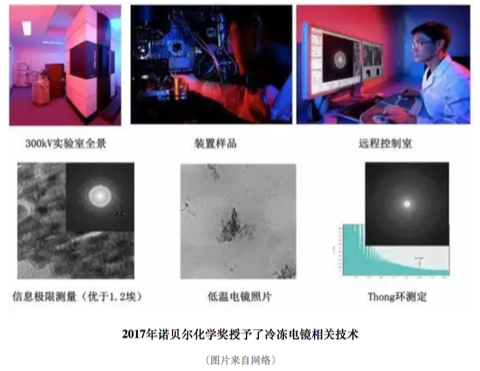
\includegraphics[width=6.67in]{images/hhcs1}

再次,这几个学科产业转化基本停留在前言里,毕业后除了年龄比同专业本科生大了不少,在满足业界要求上本质区别并不大,这进一步导致本应分流到业界服务社会的博士硕士继续留在学术界造纸,而想从学术界熬出头你看前人经验借鉴意义不大。很多人没考虑时代造就的红利窗口期而大谈特谈自己的奋斗,但要知道此一时彼一时,目前学术界的门槛比10年前高了很多,同样的奋斗强度10年前进高校很容易,现在可能去做博士后都没人要了。如果本科转行也就算了,但到了博士转行就真的是在奉献青春了,当然这可能是无法避免的。

\subsection{前景}

我们其实可以把做学术类比创业公司,博士学位前都是导师投天使轮,博士后相当于找风投,找到教职算是有投行介入吹喇叭,常任轨留下来才算上市。论文就像每年的财报,表现不好还可能停牌退市,当然不上市被收购做小老板也行,但那时候学术方向就会完全被大老板把持了。这个过程就是现状,目之所及很多人迷迷糊糊就上道了,而其中沉淀下来的所谓``人生赢家''却没有一个是迷糊的。这里我建议读下
Philip Guo 在斯坦福刚拿到博士学位后写的《The
Ph.D.~Grind》,虽然他是搞计算机科学的,但对幻化残生的研究生了解整体学术圈现状还是很有帮助的,很多观点也会有共鸣。

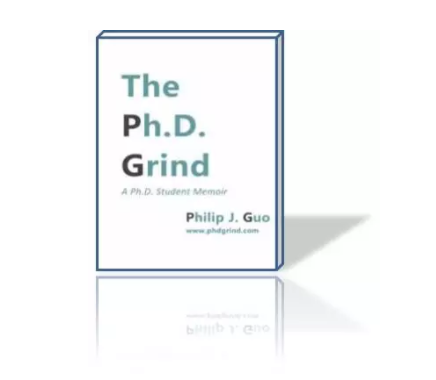
\includegraphics[width=6.67in]{images/hhcs2}

此外,我也可以给出一个基于估计的现状,如果成为院士(中国科学院/中国工程院)算达到学术巅峰的话,那么院士的选拔可以看作到达顶峰的路径。选拔方法是什么呢?两年一次,一次总共大概150人,工程科学对半分,平均一年75人。我们假定若干年后每年还是75人,且平均看每一年参与竞争的都是同年级的博士同学。而目前每年全国土鳖博士毕业生6万多人,算上海归,同一年龄组大概7万人应该比较合理。那么你看到了,你需要在同年级博士毕业生里成为千分之一的精英才算有希望。

这个似乎有点丧气,可能院士这个比较难搞,那么准院士的杰青呢?全国每年选拔200人为杰青,那么成功概率乐观估计是千分之三,杰青其实也很难了,我们再放宽到优青。全国每年选拔400人为优青,那么乐观估计成功几率大概是千分之五。我们大胆认为博士中有一半人毕业后不再从事科研工作,那么几率翻倍成为优青也要是百里挑一。即便是成为教授/研究员,我估计概率也是小于5\%的,这个基数不是所有人,而是跟你同级的博士。

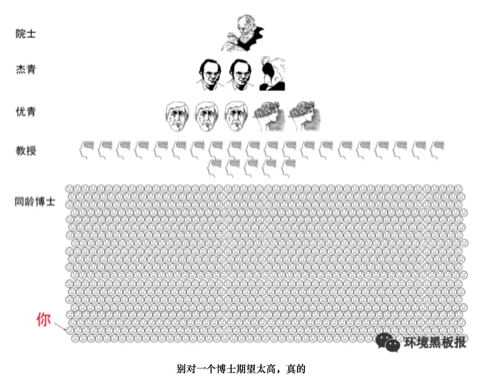
\includegraphics[width=6.67in]{images/hhcs3}

所以其实我挺理解很多劝博士毕业转行或毕业不做学术的看法的,那怕你手握博士学位,在国内想走到教授也是个p\textless{}0.05的事,大概20个人里有一个。考虑到一般博士同学同院系大概也就是20个人,如果学术水平不在前面,基本可以重新考虑下人生规划了,因为此时你选择科研就真的需要兴趣激发了,不然身边的落差会折磨你几十年。而且上面的估计有个严重的问题,那就是大量使用了均匀分布,但真实的情况却是极不均匀分布,你的师承关系跟毕业院校都会把这个分布搞得更加极端,而且后发者优势在科研里面非常常见。同时,目前教职数目趋稳,如果你没赶上窗口期大爆发,基本就是这个竞争强度了,只会更强不会更弱。具体到幻化残生这四个学科中的环境,虽然国家很重视,但在杰青或优青的名单中每年能分到多少个这都是一个巴掌数的过来的,各位可自行倒推下看看竞争强度。如果眼光放远些,其实别的学科的竞争压力也好不到哪去,但对于知识迭代比较快的幻化残生,很多压力与鸿沟可能你没毕业就已经出现了,更糟的是你毕了业才发现。


\includegraphics[width=6.67in]{images/hhcs4}

\subsection{求索}

这些现状经常搞得研究生自身怀疑人生,看着转行金融、咨询、IT的同学心有不甘;即便可以用学术理想充实的生活把自己隔离在实验室内,但走出实验室的柴米油盐变量太多,控制不来。同时,你又会很惊奇地发现,这些年报道的学术界年轻有为的青千、优青与各路人生赢家基本都是这四个学科的;而且从经费分配跟论文影响力上看,这四个学科也是超级大户;再从经济学角度去看,你会发现围绕这四个学科的仪器、耗材甚至样品测定跟论文润色服务都已经形成了成熟产业链,行业利润十分惊人。注意,这些产业是对科研进行支撑的而不是业界,如果只是这些行业高速发展而产业界没有起色,那事实上是在用纳税人的经费吹肥皂泡,不会长久。

这并不奇怪,实验学科的知识与技术更迭速度是非常快的,从走进实验室那一刻,你就会发现师兄师姐用的技术学校里根本就没教过或仅仅做了个展望,系统的学习基本上都被传帮带模式替换。如果你自己不去问为什么,大概率你师兄走的弯路你还得走一遍,你师姐画不出的图你也画不出来。更尴尬的是,有时候你会发现,如果你的想法是属于排列组合出来的,那么其实仪器公司完全可以替你做,他们不做并不是不会,而是等着收服务费,你发你的纸,我赚我的钱,各取所需。在这个场景下如果还没意识到自己的民工本质,那大概率是要做一辈子民工的。

曾经有人提过学术界存在生态位,大家各做各的相安无事,但这个想法现在看比较天真,因为现在竞争者基本都不是来自学科内,而是其他学科的入侵,如果这个问题你自己学科的人搞不定,别的学科就会过来。例如做材料的发现一种新材料,如果你觉得意义不大不掺合短期没啥问题,但做材料的表征完了得找应用出口啊,环境、生物、化学都有,技术有自己的生命力,总有人会转过去。你是无法约束某种研究只去关注自己学科内的问题的,事实上这可能是目前科学进步的一个范式:个别学科突破,带动其他学科发展。

基础学科对新技术的接受度要快于应用学科,一个常见的模式就是某个数学模型首先应用在物理领域,然后化学,然后生物,然后是边缘综合学科例如环境、医学,然后就是社会科学。当然也存在某些从应用角度出发的模型后来被应用到其他领域,金融与生命科学中经常出现这样的案例。但你应该发现一个问题,要想解决现在的问题,通常老路是不通的,要么回归基础学科,要么从别的学科借鉴,不论哪一种都需要你持续学习新知识,特别是外学科知识。有一个最简单的办法就是你去看看那些最聪明的人在用什么,然后想想能不能用到自己的学科框架里。

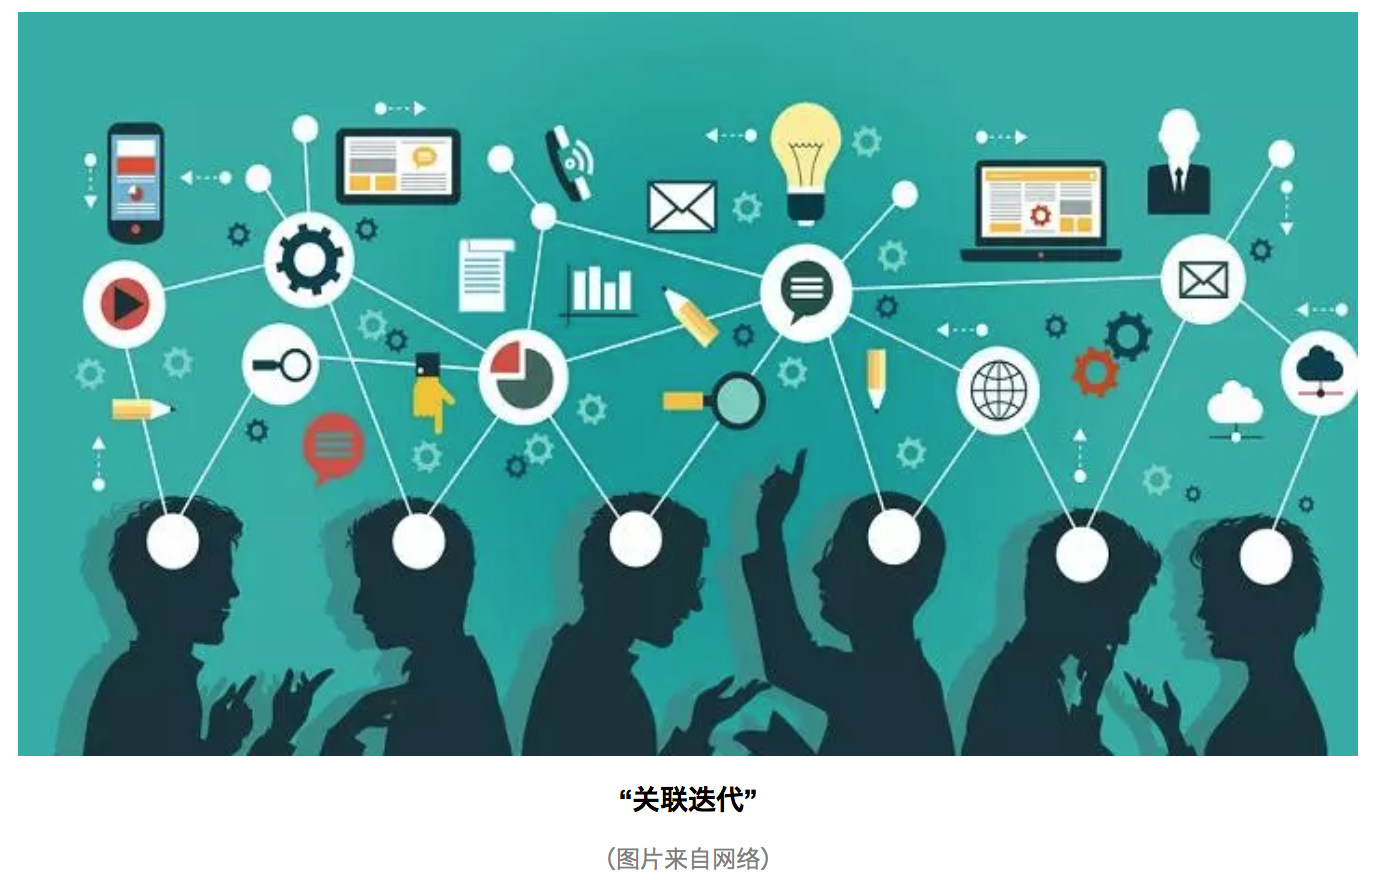
\includegraphics[width=6.67in]{images/hhcs5}

实验学科的发展有时候是很残酷的,初期势必牺牲掉一批掌握过时技术的研究生,这个国内外都很常见。通常国外业界会吸收一部分且通过较成熟的职业教育与培训体系来解决问题,国内则是依靠学术界大面积收留;这个问题的后果就是现在很多教授对于学生无力指导,看到概念就回来让研究生试,研究生自然苦不堪言,毕业后就业方向非常窄。但同样是实验学科,高能物理、生物统计的毕业生转行就相对容易些,因为可以去做码农,至少生活水平对得上学位。而很多实验学科的研究生对此并不感兴趣,甚至完全不懂,思想上停留在努力实验发论文拿教职的简单规划上,不喜欢接触社会就只接触仪器。这其实是最大的偷懒,科研是需要脑力持续投入的,如果是实验学科还要加上体力。不但要持续学习,还必须要主动学习,关心前沿,而这又与繁重的实验任务竞争着的研究生们的精力。在前沿知识的探索中没有固定的方法与理论,经验主义横行,也恰是前沿科研的魅力所在,混杂了无穷的乐趣与苦涩。

\subsection{前沿}

学科前沿是一个很模糊的东西,对幻化残生而言,教科书上的实验技术是一定落后于科研的,此时对学术前沿的感知往往要么来自文献,要么来自会议或培训,坦白说,这两个方法都具有很强的主观性,夹杂很多人的小算盘。好比你想在微信里打开淘宝链接,不是不行,就是要通过复制过程恶心你一把,但其实这种经验过程你也没啥办法。

除此之外,还有一个方法是各种文献信息学指标,例如H指数,被引率等等,但这些指标属于后验指标,你得至少等文章发表过去两三年才能开始评价,但这两三年中也会有一大把新趋势出现。另外一个方法就是自己当期刊编辑或审稿人,其实这个是很多教授的独门秘笈,因为你会比其他人早好几个月知道新研究的动向,但研究生拿到的审稿机会本来就少,高水平期刊更是不会找研究生审稿。所以其实对于很多研究生而言,想了解前沿跟他人的研究动向几乎不可能,而根据我的观察,如果同行坐到一起聊天你对新动向一无所知,那么对方也就不会在你身上浪费时间了。有些出版方跟研究机构也会发布一些热点文章,但多数基于编辑经验,并不一定准确。一个相对靠谱的方法是借鉴搜索引擎排序的思路,通过文本分析的角度从统计模型上探索趋势,这里并不是说那种通过词云这类描述性统计量,而是基于主题模型、时序分析等手段的探索分析,但手段其实是次要的,是服务你的问题的,如果问题没搞清楚,用什么都是错的。

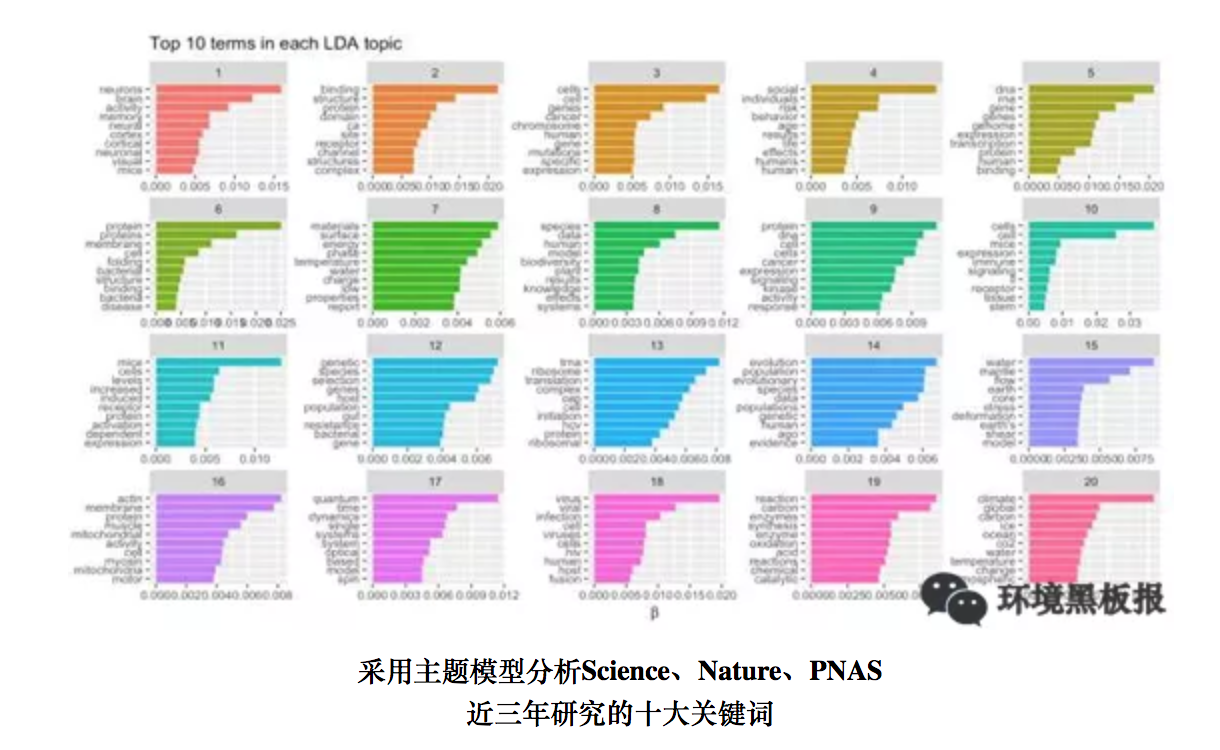
\includegraphics[width=6.67in]{images/hhcs6}

其实,对于幻化残生的研究生而言,主动了解科研趋势只是一方面,了解你自己才是更重要的。当你觉得不好时,不要总是怪罪时代跟环境,也想想自己身上的问题;当你一帆风顺时,不要总觉得这是自己勤奋与努力的结晶而忘记了科研浪潮的背后推手。随波逐流不会过的太差,但放弃思考是绝难在学术界生存下来的,不要真的幻化残生了。

师兄只能帮你到这了,剩下的,我也没想明白。

本文首发于我的科学网博客(yufree),改编首发于环境黑板报。

作者:yufree 编辑:栟

\section{北京的空气变好了,但是\ldots{}\ldots{}}

早在2009年,美国驻华大使馆便自设空气监测站,并对外发布PM2.5数据。而直到2011年以后,随着微博、微信等自媒体的蓬勃发展,一些微博大V、微信公众号开始关注并转发美国驻华大使馆的空气监测数据。这引发了公众强烈热议,什么是PM2.5也成为一时关注焦点,环保等相关政府管理部门也不得不对此有所回应。2013年,国务院发布《大气污染防治行动计划》(就是所谓的``大气十条''),提出十条具体措施,明确经过五年努力,全国空气质量总体改善。而北京随后制定了《2013-2017年清洁空气行动计划》,明确了到2017年底PM2.5年均浓度控制在60微克/立方米左右的``京60''目标。

------写在最初

今年,是``大气十条''的收官之年,北京市空气质量是否明显好转?``京60''的目标是否已经实现?带着这些问题,我们采访了北京某环境监测部门的工程师及中科院某所大气环境研究人员,并对北京市市民进行了街访。

\subsection{北京的空气质量到底变好了没有?}

北京某环境监测部门工程师(以下简称``监测部门''):从总体上来看,北京市空气质量呈现逐年转好的态势。以PM2.5为例,自2013年开展监测以来,2013-2016年PM2.5年平均浓度分别为89.5、85.9、80.6和73.0微克/立方米,下降的趋势非常明显。

根据北京市环保局发布的监测数据显示,2017年1-10月份,北京市PM2.5累计浓度为64微克/立方米,同比下降8.6\%;空气质量达标,也就是我们所说的``1级优''或``2级良''天数172天,同比增加11天。这些数据均体现了北京市空气质量正逐年好转的特征。

下图是2013年1月-2017年10月北京市PM2.5日平均浓度的热度图(单位:微克/立方米),我们可以看出,这几年,PM2.5高浓度天数确实在减少,低浓度天数在增加。

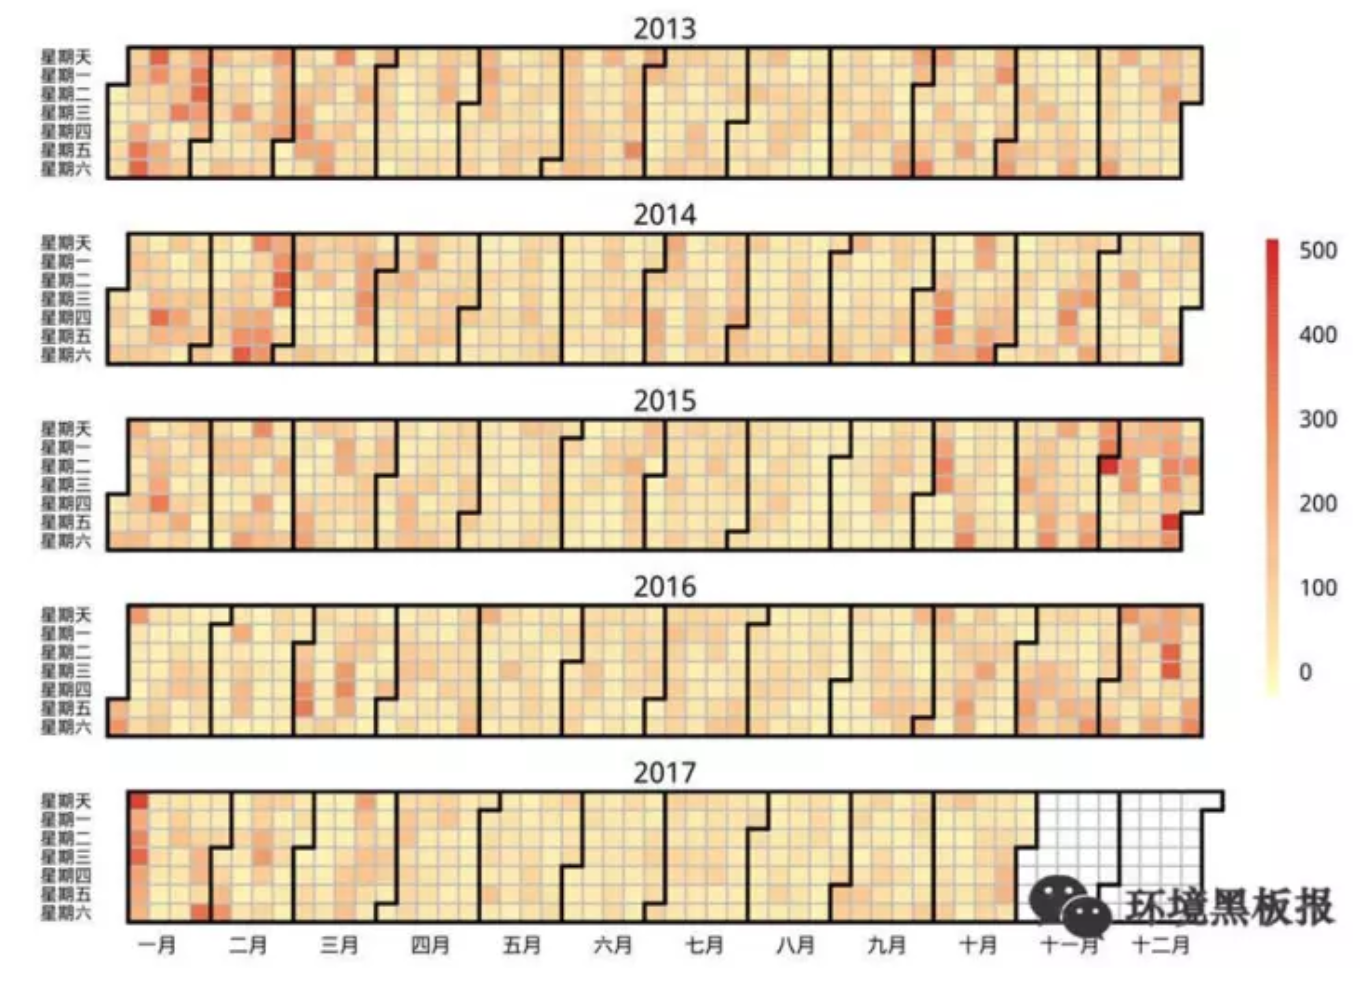
\includegraphics[width=8.33in]{images/air1}

中科院某所大气环境研究人员(以下简称``科研所''):空气质量变好还是变坏,污染物的浓度水平是一方面,污染物的成分变化更需要我们的关注。

举例来说,在1998年,北京主要遭受严重的燃煤和机动车排放混合型污染。自1998至2013年的15年期间,我们国家主要在燃煤电厂的脱硫脱硝技术方面做了很大的改进,使酸雨问题得到了控制。

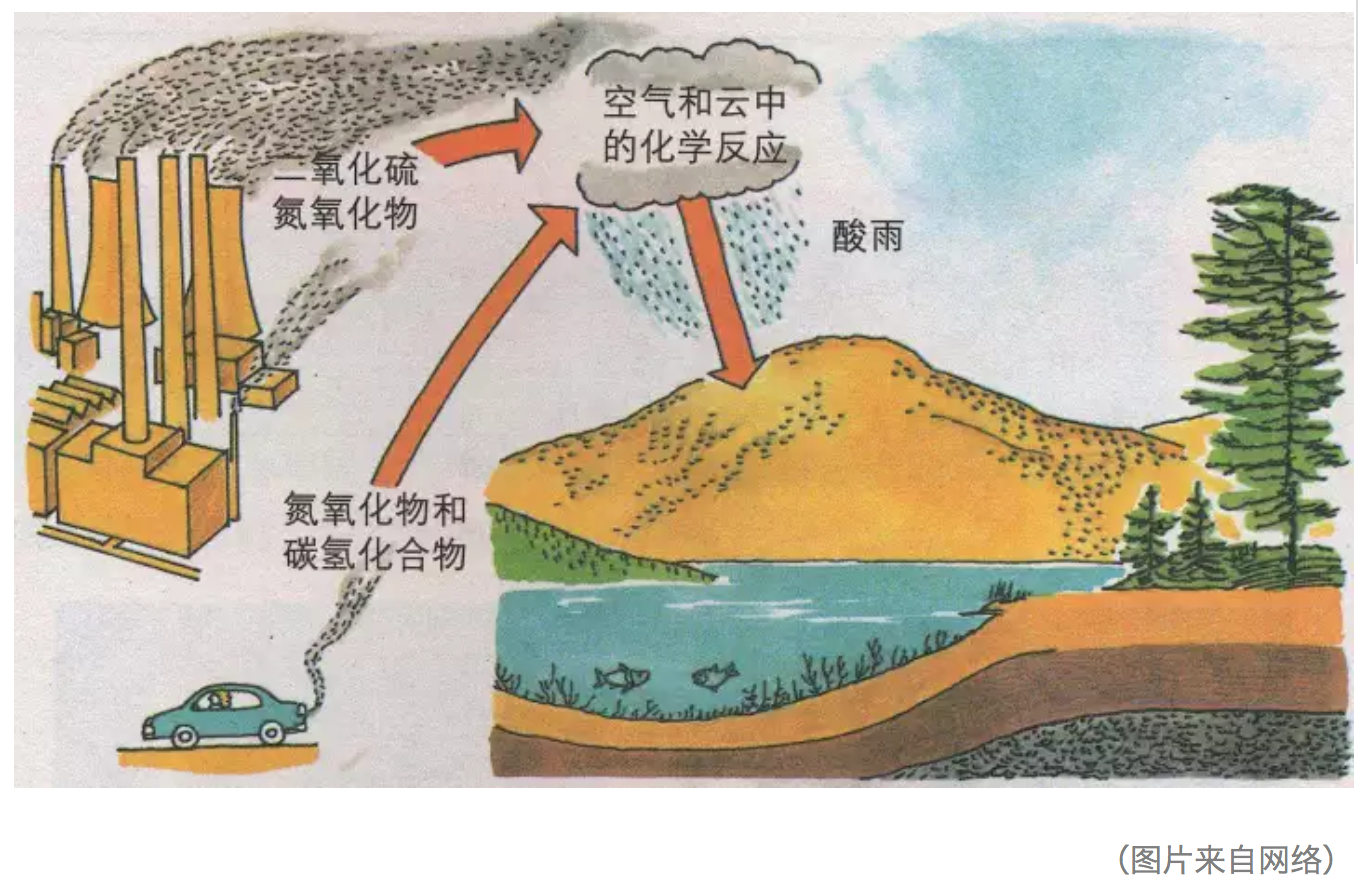
\includegraphics[width=8.33in]{images/air2}

而且,这15年期间,北京的CO、SO2、NO2和PM10的年均浓度均有显著下降,下降比例分别为58\%,78\%,24\%和42\%,尤其是CO和SO2基本稳定在国家空气质量标准值内。

但是,为什么最近几年,雾霾的问题反而更严重了呢?高效的除尘工艺只对粒径大颗粒物具有良好的去除效果,对于数量浓度较高的细小颗粒物去除率还有待提升。尤其在高湿环境下,大气中的多种污染组分如NOx、O3和光照条件促进SO2和VOC等的均相和非均相反应,促进新粒子的生成及细粒子的老化,形成成分复杂的较高浓度的细颗粒物(PM2.5)飘散在空气中,可由呼吸道直接吸入肺部,增大对人体的危害程度。同时,这些细小的颗粒物对阳光的吸收散射增强,降低大气能见度。

这几年随着环保力度加大,尤其是``大气十条''的落实,京津冀、长三角、珠三角PM2.5的浓度比2013年同期分别下降了38.2\%、31.7\%、25.6\%,下降幅度均大幅高于考核标准。``京60''目标也有望实现。

近几年,VOC的排放呈显著增长趋势,或许会成为未来大气污染治理的又一难点。

小编言:随着我们环保治理力度的不断加大,北京空气中PM2.5确实在不断减少,蓝天的数量在不断增加,我们政府下了大决心,打了场胜仗,但是空气质量是否真的变好了,可能还有待研究。

\subsection{目前,对于PM2.5浓度评价的标准使用的都是均值,如2017年,北京年均值达到60微克每/立方米左右,这样设置是否合理?}\label{pm2.5201760}

监测部门:目前的标准,使用的是均值,每日空气质量评价参考的是日均值,年度目标的完成情况参考年均值。各行各业很多和实际生产生活相关的标准都不需要特别精细化,虽然说设立置信区间能够更精细化,但是在当前的实践中可能比较有难度。标准就是个标尺作用,要满足大部分需要,在满足日常需求上,我认为用均值就够了。不过科学的标准更应该是根据人体健康效应来设置。

科研所:我不认为均值是一个很好的统计量,打个比方,如果只用一个标准值去衡量,那就相当于默认均值背后的分布或者污染特征是一样的,但实际数据的分布并不一样。如果能够精细化一些,可能会更加准确,说服力也更强一些。当然,这也是当前科研出现危机的一个例子,现实的复杂并不适合用简单统计量来描述。

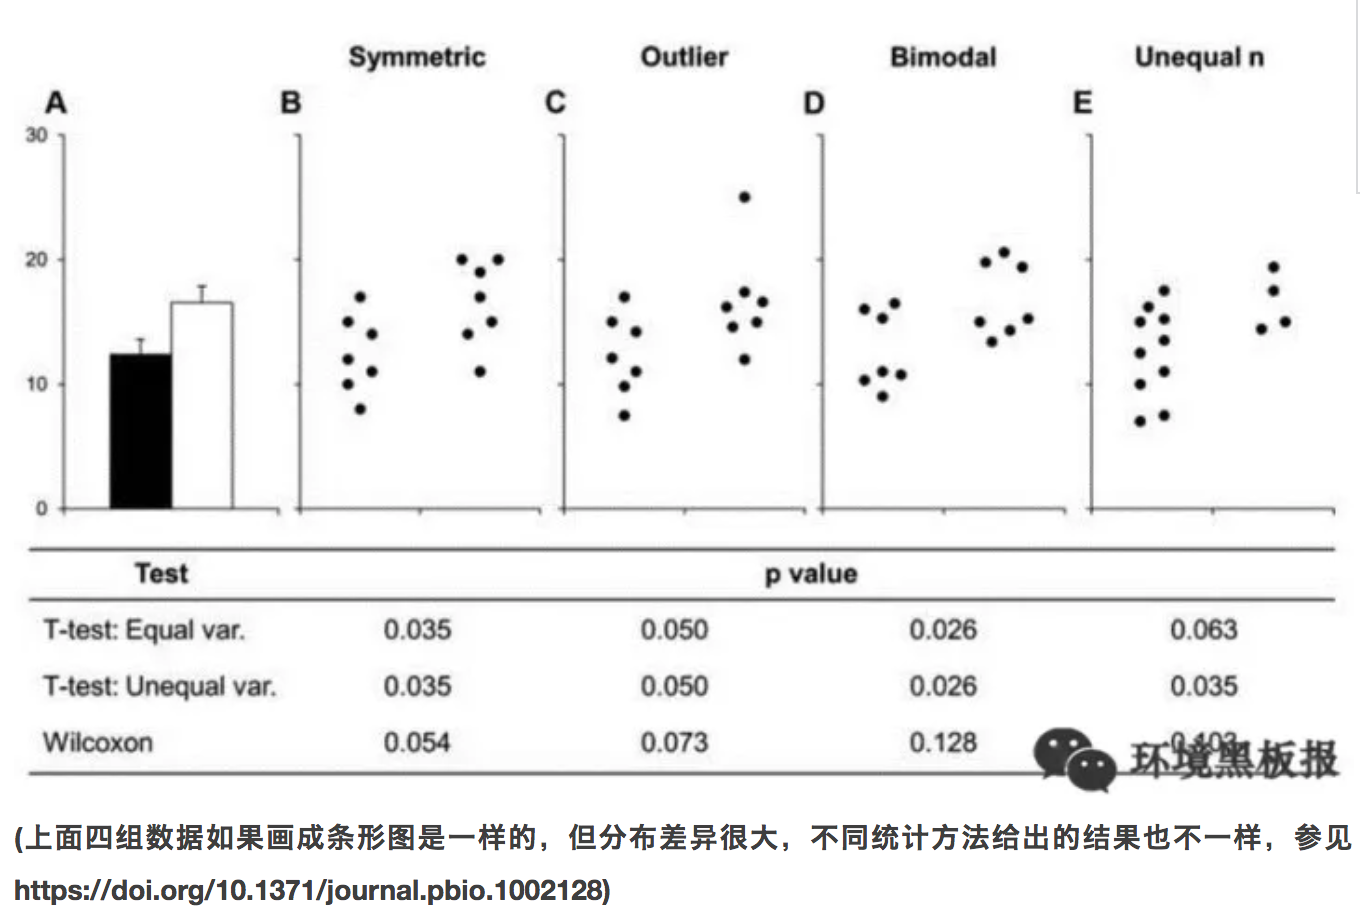
\includegraphics[width=8.33in]{images/air3}

现在环境监测能力越来越强,获得的数据越来越丰富,加上越来越先进的数据处理手段,有实现精细化展示的可能性。标准的制定最好通过置信区间来定义,例如考核指标改为90\%的分时浓度区间,也可以考虑工作日与双休日制定标准。

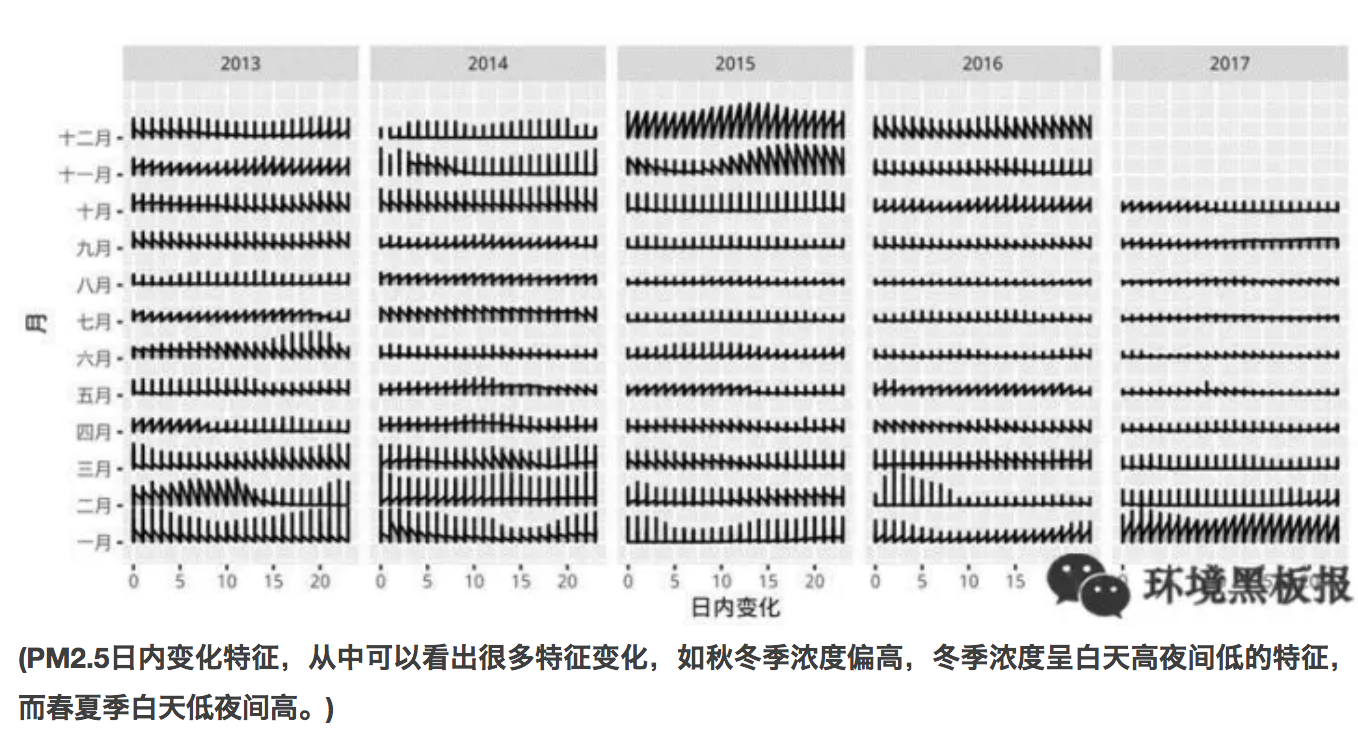
\includegraphics[width=8.33in]{images/air4}

小编言:均值作为标准,应用和管理起来或许会很方便,但是会隐含一些我们看不到的分布特征,而这些特征对于精细化管理大有裨益。

\subsection{按照《北京城市总体规划》(2016-2035年)要求,到2020年PM2.5浓度下降到56微克/立方米左右,对此,您持何种态度,判断依据?}\label{2016-20352020pm2.556}

监测部门:我对此还是持乐观态度的,主要原因为:(1)目前的高压态势环保治理已经成为常态,而不是部分时期采取的临时措施,污染源减排力度将会持续加大。(2)国家正积极加大能源结构调整,目前清洁能源的使用率和使用范围越来越大。(3)民众的环保意识越来越强,自身参与环保的行动也越来越多。在政府和民众的不懈努力下,北京市PM2.5浓度会越来越低。

科研所:对于这个观点,我持乐观态度。首先,政府、民众都很关心,科研人员也在污染源解析、气象模式预报、大气污染追因等方面做了很多的研究工作。其次,治理污染需要一个过程,在2015年以前,重点在酸雨的调控,近几年,重点在PM2.5的调控,未来还有VOC和O3问题也需要解决。根据目前的数据和政府的决心来看,我是持乐观态度的。

小编言:对于未来,我们多是持乐观态度,一方面我们对现在的政府充满了信心,``绿水青山就是金山银山''理论正在引领新实践,另一方面我们自身也深感美丽生活环境的重要性,环保意识不断增强。

听了政府监测部门和科研机构人员的回答,我们已经感受到了政府和研究机构在改善北京空气质量方面所做的努力。那么作为北京市居住的老百姓,作为空气质量改善的最直接受益人,他们的感受是怎么样的呢?

\subsection{您好,您觉得北京的空气变好了吗?}

蓝天:感觉今年蓝天确实比去年多了,是不是跟今年风多有关系啊。不过也听说最近环保搞的力度挺大,又是督察又是巡查的,空气污染严重还问责,今年还轰轰烈烈的搞了煤改气,听说周边农村里煤不让烧,气供不上,挨冻了都,好在听说环保部紧急发文,让一些没改好的地方接着烧煤。今年天儿好可能这些治理法子还是起了作用吧。

白云:感觉今年重雾霾好像是好了一点,以前雾霾严重的时候,窗户外面都几乎看不见。其实我对雾霾真是没怎么关注,感觉对自己影响不大,主要是考虑到孩子,希望每天都可以看到蓝天,这几年的雾霾让人有些麻木了吧,到哪里看到雾霾都不觉得吃惊了,反而连续出现蓝天倒是觉得不可思议。

青山:这个我还真关注了,毕竟跟咱北京人儿息息相关么。北京现在空气肯定是在慢慢变好,但是大家感觉不强烈。感觉政府宣传的不好,一方面是老百姓不信,另一方面政府没有转变思维,还是封堵,而不是疏通,预警措施也不够。

\subsection{按照目前北京市环保局网站公布数据,北京市今年很有可能达到年均值60微克每立方米左右,北京市空气质量逐年改善,您对此怎么看?}\label{60}

绿水:其实吧,我不清楚60微克是啥概念,天天听人说,也没有人科普过,如果说就是雾霾好一点,今年感觉是比去年强点,但要说强多少,也没有吧,前两天不还雾霾来着。

阳光:达标能怎样,数据可以求平均值的,总共有个30天极其严重,而其他天数全是好的,一平均不就是好了,但是老百姓的感官还是不好的。

鲜花:恩,现在政府抓环境抓的紧,我们那片好几个小工地都关了。政府立了指标,老百姓就好监督嘛。而且现在市长是搞环境出来的,又是从环保部过来的,我觉得在改善北京空气方面,还是能有所作为的。

小编言:看来,民众的感受也是因人而异啊,不过总的来说,政府的努力还是得到了认可,民众提出质疑的同时也对政府对科研部门寄予了厚望。

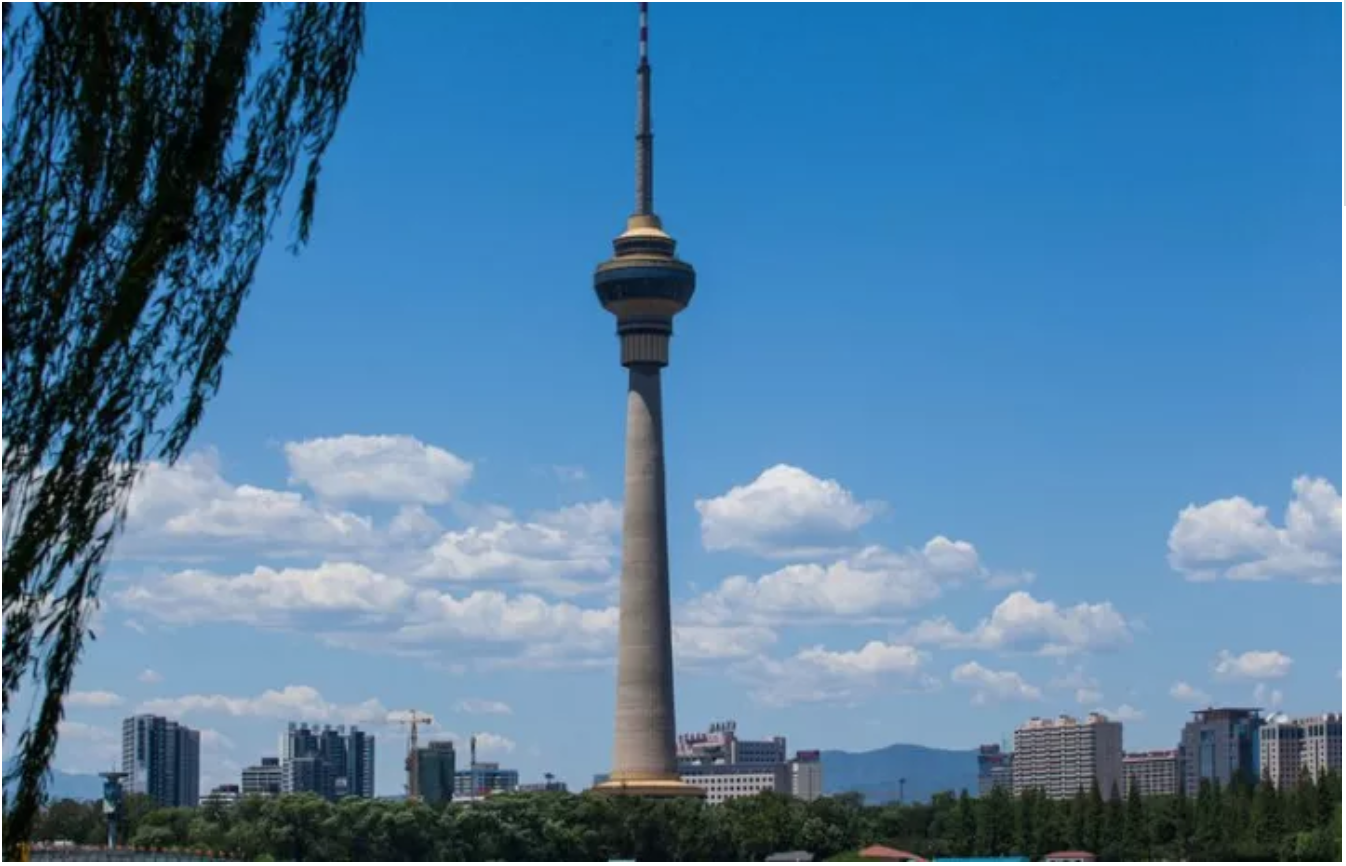
\includegraphics[width=8.33in]{images/air5}

经过几年的努力,北京的空气改善明显,但是否有新形式的污染物出现危害公众健康,是否在目前认为的质量改善背后隐藏着其他的隐患,作为政府工作人员还是科研工作者亦或是你我,都仍需负重前行,不忘初心。

作者: 次要男主角 校稿:周宁,王小咖 图片:yufree 编辑:竹而乐

\section{一滴水的故事}

曾几何时,一滴水随着千万个同伴出现在这个星球。他们开始塑造这个星球,改变着地貌,孕育着生命。人类从出现的那一刻起,就开始了与水相爱相杀的历史。从两河流域的空中花园到尼罗河流域的金字塔,从马拉松的烽火到牧野之战的硝烟,水,孕育了地球最初的文明。同时,人类早先的传说,从诺亚方舟到大禹治水,又无处不在昭示着人类对水的敬畏。

水与人类的相爱相杀一直在进行着。有一滴水躲在茶壶里变成了蒸汽,告诉一位叫瓦特的人这样的力量可以推动机器运转,于是推动了轰轰烈烈的工业革命;有一滴水和同伴们一起构成了江、河、湖、海,让人类可以物流南北、货往东西,文明的火种得以靠水传播。

人类使用着水,也污染着水;净水养育着人类的同时,污水却时刻威胁着人类,这样的相爱想杀更是直接催生了我们的专业------环境科学与工程。此刻我们对水充满敬畏,毕竟水撑起了整个产业链上的勤劳的人们。水进入大气在不利的气象条件和污染物参与的情况下,形成雾霾,这一点我们在《混沌的冬日》里已经写过;水进入城市,若无法正常下渗、排除,则形成内涝,这直接催生了海绵城市的建设思路,这一点我们在《城市之殇》中已经展现;即使不听话的、因污染而变坏的水,工程师们不死心,坚信每一滴水都是清纯的,于是我们人类建立了污水处理厂,通过活性污泥法和生物膜法等工艺,使受污染的水改头换面,还清还纯,而这在《污师私房菜》中,我们也有所提及。

地球的水储量是巨大的,然而淡水资源却是如此的稀缺,环境工程师们在累死累活守护净水的同时,一个``开源''的灵感开启了水资源的另一段神奇之旅:

\subsection{海水淡化}

海水淡化方法主要分为热法和膜法。

热法:海水的盐度很高,直接饮用只会越喝越齁,但早在公元前1400年,海边的居民便学会了在锅内把海水加热到沸腾,使海水蒸发变成水蒸汽,盐分留在锅底成为垢,并使水蒸汽遇冷成为可饮用的蒸馏水。这也是今天常用的蒸馏法海水淡化的原型。而现代常用的热法海水淡化主要有多级闪蒸和低温多效两种。

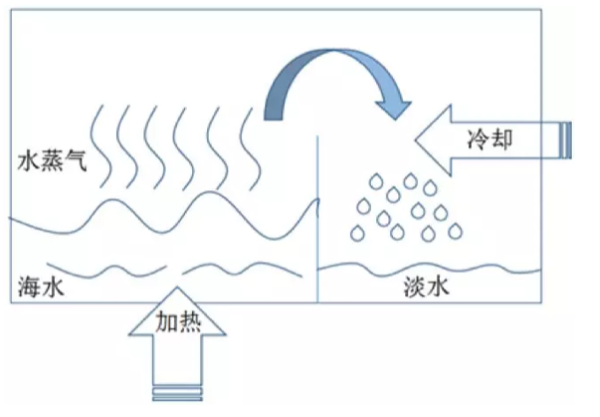
\includegraphics[width=8.33in]{images/seawater1}

膜法:1950年美国佛里达大学瑞德(C.E.Reid)教授在无意间发现了一个奇怪的现象。他观察到海鸥在海上飞行时从海面啜起一大口海水,隔了几秒后,吐出一小口海水,这个现象引起了他的思考。后来经研究发现,海鸥体内有一层薄膜,该薄膜非常精密,海水被海鸥吸入体内后,经过压力作用使水分子穿透薄膜转化为淡水,而含有杂质及高浓缩盐分的海水则吐出嘴外。于是,受此启发,瑞德教授提出了反渗透的基本理论。反渗透膜如同一只特殊的过滤筛子,在压力下过滤掉了水,而留下了盐(看到这里我觉得瑞德教授至少不是一个喜欢吃野味的人)。运用这一原理,我们就可以利用反渗透膜从盐水中获取淡水了。

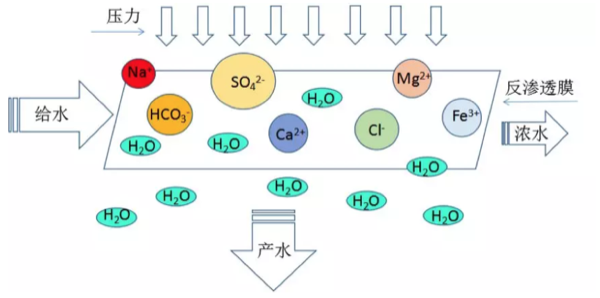
\includegraphics[width=8.33in]{images/seawater2}

我国人口占世界22\%,淡水占有量却仅为8\%,世界排序名列109位,是世界上12个严重贫水的国家之一。而海洋中蕴藏着丰富的淡水,其总量约占海水的97\%,相当于13.3亿立方公里之多,是一个巨大而又稳定的淡水储库。海水淡化作为水资源的开源增量技术,具有稳定供水、应急供水和战略性供水的特点,是解决沿海水资源短缺问题的重要途径。笔者收集了我国沿海地区人均水资源情况,发现沿海地区由于经济发展水平和人口密度较高,缺水情况反而高于全国平均水平,形成了靠水没水的情况。海水淡化成为了一些沿海地区解决缺水问题的关键手段之一。

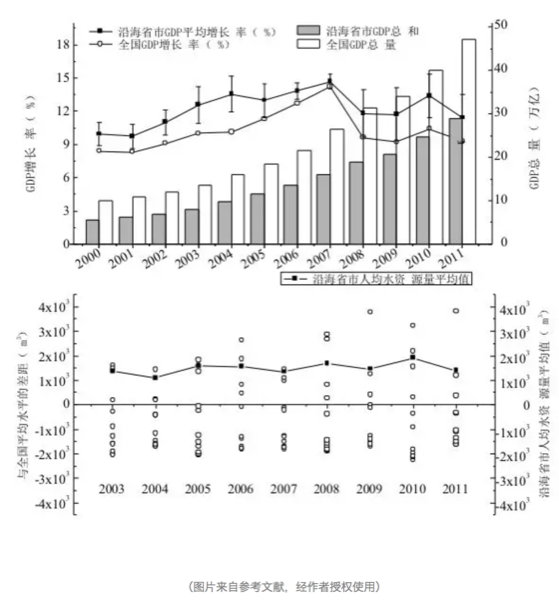
\includegraphics[width=7.76in]{images/seawater3}

我国海水淡化的历史始于上世纪五十年代。至2015年,全国总产能已经超过百万吨,约为全球海水淡化总产能的2\%左右。随着经济的发展,我国在国际海水淡化市场的比重逐渐增加。如下图所示,我国在这一年的产能增长约为中东地区的一半左右。中东地区存在一些自然条件上的限制,促使他们更加积极地开发海水淡化技术,因此中东地区历来是海水淡化最重要的市场,所以我们国家海水淡化产能比不过这些土豪真的不丢人。

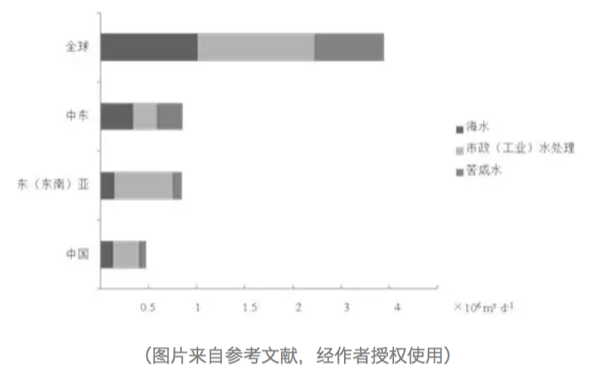
\includegraphics[width=8.33in]{images/seawater4}

目前我国已建的海水淡化产能主要集中在辽宁、天津、河北、山东等北方省市,这四省市产能占我国海水淡化总产能的81.9\%(2014年数据,见下表);与此对应的是不同省份对于海水淡化的关注度,下图是来自海水淡化的网络搜索指数,排行前五分别是北京、广州、浙江、江苏、山东,从中不难看出,海水淡化的关注度和接受水平也与地区的经济发展状况息息相关。

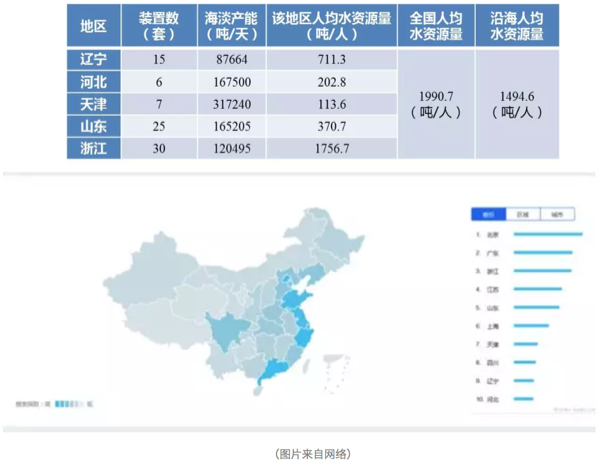
\includegraphics[width=8.33in]{images/seawater5}

2016年12月,国家发改委和国家海洋局联合印发的《全国海水利用``十三五''规划》指出,到``十三五''末,全国海水淡化总规模拟达到220
万吨/天以上,其中沿海城市新增海水淡化规模105
万吨/天以上,海岛地区新增海水淡化规模14
万吨/天以上。而海水直接利用规模拟达到1400
亿吨/年以上,海水循环冷却规模达到200
万吨/小时以上。新增苦咸水淡化规模达到100
万吨/日以上。海水淡化装备自主创新率达到80\%及以上,自主技术国内市场占有率达到70\%以上,国际市场占有率提升10\%。相信未来海水淡化会有更快的发展。海水淡化项目在某种程度上是一种基础建设项目,与各级政府的施政方向密不可分,所以虽然国家出台了一系列的规划政策,具体落地还是需要很长一段路。

\subsection{后记}

2010年,我们像一个一个水滴汇入了中科院这个汪洋大海,拥有了这片汪洋大海里的化学物质。随着时间的推移,我们又流到了其他地方,在各自的岗位上吸收了新的化学物质。不同物质间的反应总能产生新的物质,所以我们决定讲我们的源,讲述我们每一滴水的故事。

作者:yy 校稿:胜利屯支书,看透 编辑:栟

\section{可持续社区建设案例------北京当代MOMA公寓}\label{moma}

可持续发展是一个比较容易引起人们困扰的概念,从1987年《我们共同的未来》出版以来,可持续发展的概念已经走过了三十年。目前全世界人们最公认的可持续发展的核心思想就是``既能满足当代人的需要,又不对后代人满足其需要的能力构成危害的发展''。

2015年6月5日,联合国发布了题为《Transforming our world by 2030: A new
agenda for global
action》的报告,这是联合国首脑会议对于2015年之后全球发展的整体规划和展望。可持续发展目标的设立源自于被全世界人民所认可的可持续发展理念,以消除贫困和不平等、保卫地球、创建包容经济增长空间为基础构架,由17个总目标和169个子目标共同组成了一整套覆盖社会、经济、环境三个关键维度的全世界发展目标。

其中,目标11为可持续城市与社区,以建设包容、安全、有抵御灾害能力的可持续城市和可持续的人类居住社区为核心目标。在可持续城市与社区的大目标之下,设计了7个子目标和一个整体目标从多个关键方面提出了在城市和社区尺度可持续发展的要求,如住房与交通的需求,城市建设力度的要求,城市对人类的负面环境影响如空气质量、城市废弃物等的要求,以及城市居民能够在社区中享有足够的绿色公共空间和社区服务的要求。

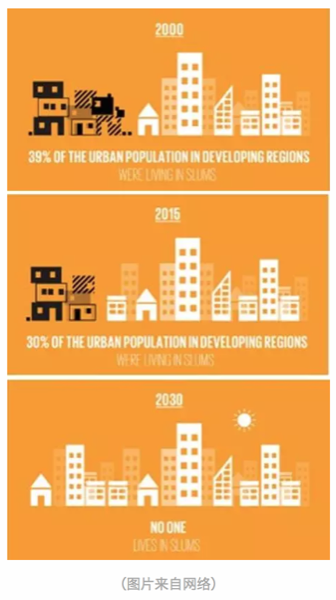
\includegraphics[width=4.67in]{images/moma1}

社区是一个非常有意思的概念,当我们以人类聚居的角度去看,社区可以看成是城市最基本的组成单元,也是连接城市和单体建筑的人类聚居栖地,不同于家庭的血缘聚集性,社区是用一个划定的区域把一群没有血缘关系形形色色的人类和一堆单体建筑圈定在了一个概念里,在社区里往往能找到一个城市的大部分商业和社会服务功能,也能看到城市生活的最完整的缩影。在大多数情况下,城市的政策和举措需要在社区层面得到落地和实施。

我们现在日常居住的居民小区、商业楼盘甚至早一些年的街道居民委员会管辖片区,都是最为常见的社区。随着城市社会经济的不断发展,社区可以涵盖的概念也越来越广泛,商业与居住型公寓并存的CBD区域、特色产业园区及周边物业、甚至是特色小镇,谁又能说这些都不是社区的代表?这些新型地产类型的兴起,也从另一个方面极大的丰富了社区的概念,也让可持续社区的建设与实践越来越具有现实的意义。可持续社区的理念强调现在和未来、生活和工作、安全性和包容性,生活品质和环境保护等统筹协调,规划合理、建设和运营良好,为社区居民提供平等的机遇和优质的服务。

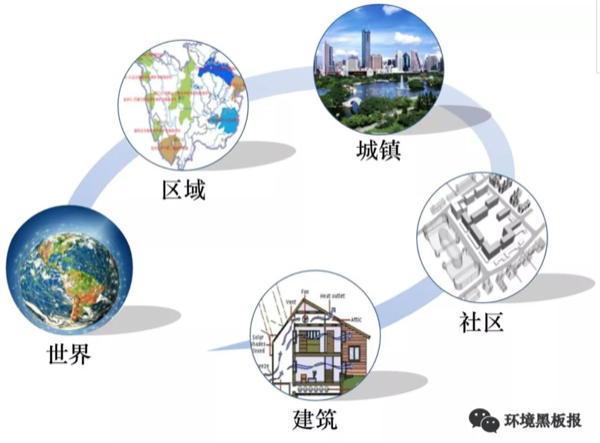
\includegraphics[width=8.33in]{images/moma2}

\begin{quote}
当我们讨论如何去建设可持续社区的时候,一定会有一个问题始终萦绕在设计者、建设者、管理者和居住者的心头,那就是,什么样的社区是可持续的?
\end{quote}

嗯,负责任地告诉你,这个问题,其实全世界的研究学者、政府和企业想了三十多年其实也没有非常的想明白。为什么呢?可持续发展本身就是一个没有最好只有更好的概念,基于可持续发展的概念延伸而来的一系列的理念和要求,都在不断地要求着更加优化的发展方式。节能的要更加节能、贫困消除的要不断富裕、性别平等的要更加平等,等等等等。所以,当我们考虑可持续社区的建设实践的时候,其实就不要太纠结于到底怎么样是可持续的了,换个角度想一想,什么样是不可持续的,然后尽力避免是不是一个更为简洁的思路呢。

因而,可持续社区的建设,很多时候是遵循着避免不可持续性的思路来进行实践的。在可持续社区建设实践中,有这么几个点是比较值得关注和注意的,同时也可以看成是一个社区建设``从摇篮到成长''的生命周期,从社区建设的空间布局开始,就要求以能够持续发展的思路和原则进行设计,建筑及室内环境建设、室外环境建设、基础设施建设是从社区的实际建设方面的可持续性要求,而当社区建成之后,居民生活方式引导和社区运营管理的可持续性就是社区成长成熟过程中的可持续性的体现。

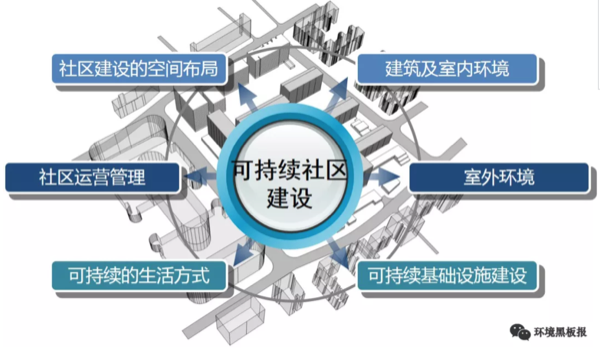
\includegraphics[width=8.33in]{images/moma3}

在可持续社区的建设实践方面,大家还是走的比较靠前的,毕竟嘛,物质基础的建设总是比精神层面的提升要来的简单一些。目前国内可持续社区相关的指标主要来自于发改委、住建部和环保部,大部分指标规定了可持续社区当中的某一个或某几个部分,而并非是可持续社区的全部内容。社区的可持续性主要聚焦于社区生态环境的可持续性,对于社区的社会系统和经济发展的可持续性的要求相对较少。从可持续的理念出发,社会公平、经济繁荣、环境优美是可持续社区三个必不可少的关键点。联合国环境规划署与佳粹(中国)环境发展促进中心共同发布的《可持续城市与社区评价标准导则》,是参考了可持续发展目标11,并同时借鉴国际标准化组织在社区可持续发展指标体系以及国际最佳范例,提出的有参考价值的发展目标、关键绩效指标和国际化考量标准,《可持续城市与社区评价标准导则》导则关于可持续社区的评判包括六个方面:可持续建筑;包容的社区服务与设施;宜居的社区景观;经济生产力;安全;自豪、高知社区。

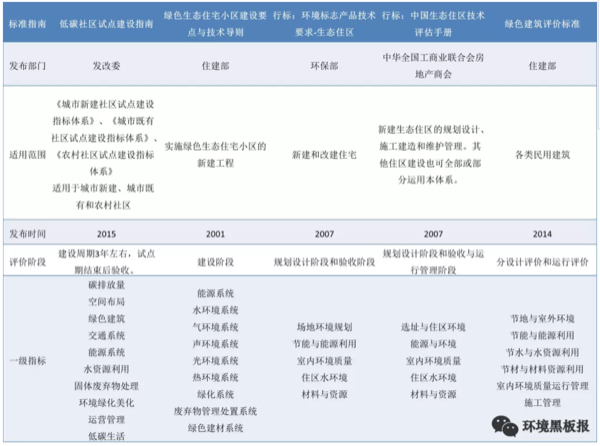
\includegraphics[width=8.33in]{images/moma4}

来看一个栗子吧。

\subsection{北京当代MOMA高端综合公寓}\label{moma}

北京当代MOMA高端综合公寓,不仅包括若干栋公寓住宅,还有影院、图书馆、酒店以及各种餐饮、娱乐中心,生活设施与休闲商业都非常完备的一个社区,为什么拿它来做一个可持续社区建设的例子呢,因为有人这么评价它的,``它构建了一个新的社区模式,将城市空间从平面、竖向的联系进一步发展为立体的城市空间,并大规模使用可再生的绿色能源,既节能又省地。它也探索了一种未来城市的生活新模式,将居住、工作、娱乐、休闲、交通结合在一起,通过空中连廊交错相连,必然加强邻里间的联系与交流。从建筑学上讲,我们依稀看到大师理念的传承与发扬,从社会角度讲,它为中国的21世纪居住树立了一个新的典范。''这是可持续社区的一次很有意思的探索实践。

在社区建设初始的设计中,以一副珍藏在俄罗斯圣彼得堡历史遗产博物馆内的镇馆画作为创意灵感(``野兽派''画家马蒂斯创作于1910年的画作《舞蹈》),同时加以北京``胡同''与``四合院''为改造元素,设计出空中连廊作为公共空间,以打造``城中之城''设计概念展开。通过连环的空中长廊将8栋公寓建筑连接在一起,加上一栋艺术酒店和一座多功能水上影院,构成一个立体的建筑空间。在建筑的外立面采用磨砂氧化铝板减轻高密度、大体量建筑的压迫感。整个社区的设计焦点是穿越空间的体验,将大楼之间的动作、时机和序列整合考虑,视点随着缓坡、转弯改变。而电梯的转换,更犹如电影里的切换镜头,从一个楼层到更高楼层的通道,平移过一些不同变化的周边景色。

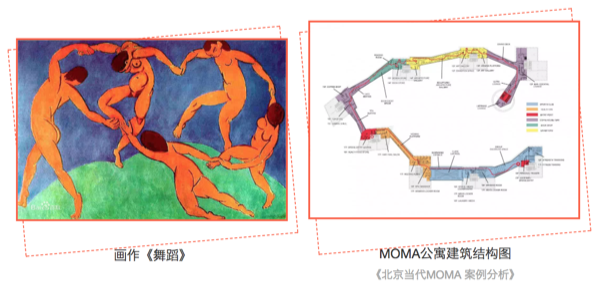
\includegraphics[width=8.33in]{images/moma5}

在社区的具体建设中,有非常多的可持续性理念的体现,这个社区以``永续建筑''的理念来践行了建筑本体的建设和施工,主要包括恒温恒湿、新风置换、地源热泵、中水处理系统等。这些体现建筑可持续性细节的系统设置,更多的是从居住者的切身感官出发,保证着每个人在房间里都能感受到一种舒适的环境,恒温恒湿和新风置换系统就是从体感上给居住者这样的舒适享受。同时,当代MOMA的这些系统设计还遵循着可持续性对于资源节约和因地制宜的要求。

恒温恒湿系统采用预埋管材的水循环系统,来保证室内温度常年保持在恒定的22-26℃,不仅不会破坏室内装修,甚至连风和噪音也感受不到。这样通过水循环系统来打造室内恒温恒湿的居住环境,不仅能让居住者感受到最极致的体验,更是一种非常节约能源和水资源的方式。

新风置换系统是将经过了过滤、除尘、灭菌、控制温度和适度的新鲜空气从房间底部的送风口送入房间,经过室内循环之后从房间顶部的排气孔排除,利用空气上升的自然原理,不仅杜绝了空气之间的交叉污染,也是以非常节能环保的方式保证了即使在北京大雾霾天的情况下也能实行对室内空气质量的要求。

地热源泵采用的复合式能源系统,是通过地下100米以下的垂直换热器以矩阵的格局分布在地下车库的地板下,与土壤进行热交换后再向上传递供热或者供冷,将对周围环境的影响降低到了最少,并且充分地利用了地下温度,几乎接近于可再生能源。

中水处理系统采用膜生物处理的技术,将社区内每天产生的大部分厨房以及洗浴废水作为中水水源,处理之后全部回用于社区商业、影院、图书馆以及部分楼座的冲厕用水,剩余的用于绿地灌溉、道路浇洒以及景观补充水等。

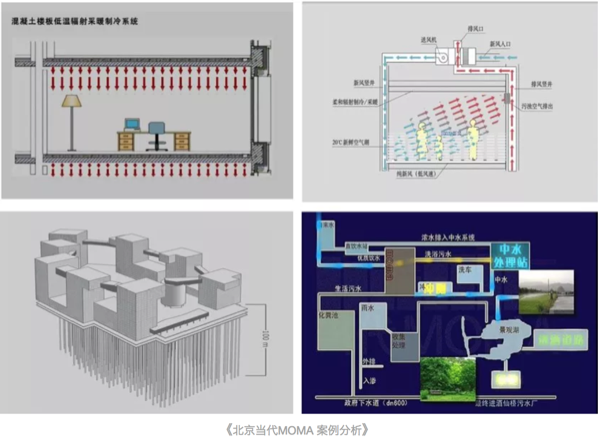
\includegraphics[width=8.33in]{images/moma6}

在社区尺度的可持续性建设中,有非常非常庞杂的关键节点和细节可以体现,从能源节约、资源利用、废弃物处置等诸多实际的物质节约的诉求,到社会公平、社区和谐、环境友好等精神层面的追求,无一不体现着可持续发展目标。限于篇幅,我们就重点了解了一个可持续社区在设计和建设方面的可持续性的体现。我们能看到,可持续社区的建设其实是渗透在社区生活方方面面的一个持续性改善过程,从国家和城市的规划布局,到社区建设的具体实践,再到社区居民身体力行的改善,每一个角色都对可持续社区这个目标的实现贡献着自己的力量。这其中,诸多标准帮助规范着社区建设的实践行为,价值导向指点着社区居民的日常生活,而城市上层的整体规划是引导可持续社区建设实践的方向标。

作者:爱杯子的王小咖 校稿:yufree,大石 编辑:兔
配图:爱杯子的王小咖,栟

\section{小秸秆,大问题}

2017年11月,演员孙艺洲拍戏途径哈尔滨,被郊县烧秸秆的烟熏味儿呛到流泪,随后在微博上抱怨:为什么一个白天空气质量优良的城市到了夜晚就空气爆表?为什么?怎么办?这个问题并不算新,但当它被一个拥有一千多万粉丝的耿直boy问出来的时候,还是结结实实触到了很多人的痛处。

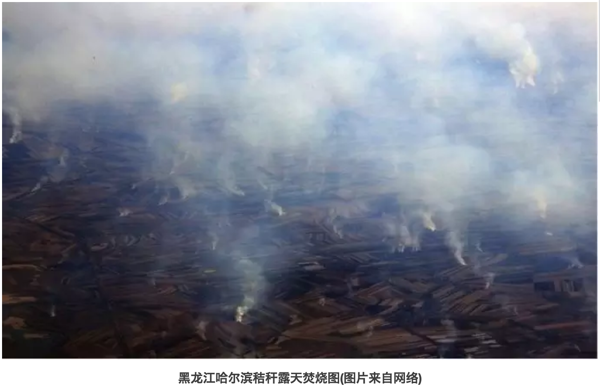
\includegraphics[width=8.33in]{images/stalk1}

在哈尔滨,把孙艺洲呛到流泪的是秸秆焚烧产生的颗粒物。每年秋收以后,庄稼被打捆、加工、再被送到每个人的餐桌上,算是完成了自己的历史使命;但秸秆这种副产品却被留了下来。

在田间地头,常常可见成垛的玉米或者小麦秸秆,勤快点儿的农户,将其垛得整整齐齐,也算是道风景;懒一些的,堆放得毫无章法,影响观瞻。

其实这个时候农民是真的忙。每年10-11月,是我国
``秋收秋种''期,各级农业部门一级战备、高度紧张,密切关注天气变化和降雨量,一轮又一轮的``紧急通知'',为的是指导农民收得时机合适,种得不早不晚。因为只有这样才能保证丰产丰收。

我们大东北黑土地在这个时候是收玉米种小麦,秋收整地追求``深、净、细、实'',小麦播种要在适宜播种期抢播早播。收下来的玉米秸秆无处可放,尽管我国80年代起就出台各种秸秆禁烧的相关规定,禁烧态势越压越重,但比起秸秆处理的经济压力和劳动力需求,很多农民不由自主就选择用``一把火''解决问题。

不烧不行啊,秸秆太多了。1991年我国秸秆产量为6亿多吨,经过了粮食总产量的``十三连丰'',到2015年,秸秆产量为10亿多吨。多出的秸秆总量为4亿多吨!什么概念呢?如果把这4亿多吨秸秆以100根为一扎首尾相连,能绕地球赤道转325000圈\ldots{}\ldots{}

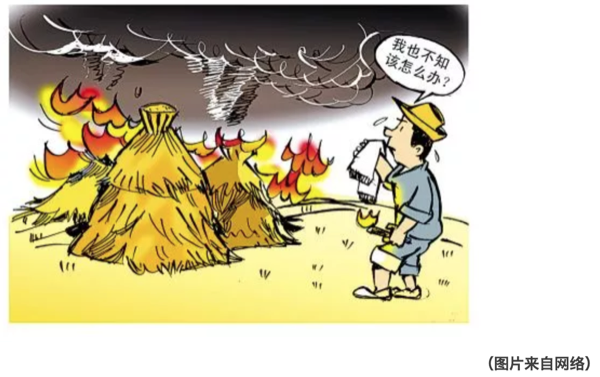
\includegraphics[width=8.33in]{images/stalk2}

不烧不行啊,农民家里实在没人。壮劳力都出去打工了,只剩下老人和孩子,尽管乡里承诺可以集中处理,那也需要把秸秆运输到集中处理点,老人孩子不会开车,没有工具,再好的政策也解不了眼前的急。

但烧秸秆的确是后患无穷。农作物光合作用的产物有一半以上保留在秸秆里,它富含氮、磷、钾、镁和有机质,秸秆大量集中燃烧的过程也是一种剧烈释放能量和物质的过程,周围环境根本无法在短期内消纳这么多的释放物,大气污染因此产生。

跟燃煤锅炉引起的污染不同,秸秆焚烧的主要产物是颗粒物、一氧化碳、二氧化碳等,对城市和乡村的低空空气影响更为直接。然而在大气污染研究领域,秸秆燃烧对雾霾的贡献一直颇有争议。

撇开具体贡献率不谈,稍加研究便可发现:在10月和11月的秋收期,从华北到东北(每年秸秆主要燃烧区),雾霾符合低硫份、高悬浮颗粒物、连片集中爆发的特点。

换句话说,叠加了大规模的秸秆焚烧,使得轻中度采暖季雾霾立刻升级为大范围重度雾霾。环保部10月期间的卫星遥感巡查监测数据分析表明,在16个省(区)共监测到疑似火点1583个,比2014年同期增长74.5\%,也的确证实了秸秆燃烧对雾霾的推波助澜``功效''。

所以,怎么办才好?秸秆问题和我国的大多数农业问题一样,工程浩大、解决起来困难重重。

目前秸秆的综合利用工作虽在稳步推进,但仍存在很大问题:一是秸秆还田成本高,运营公司与农户缺乏主动性;二是农民缺乏必要的技术支持,导致秸秆无法真正实现废物利用。

就东北地区来说,冬季气温偏低,秸秆还田要想充分被土壤消纳,必须使用进口农机深度翻耕,进一步增加了还田成本和土壤压力。说白了,东北地区黑土地耕作土层只有20厘米,想翻耕30厘米好让还田秸秆快速腐烂,需要钱,需要时间,需要人力,需要对新茬农作物减产的心理预期。

与这些困难形成对比的是,政府部门越来越强硬的禁烧手段。自1997年起,我国开始重视秸秆禁烧和综合利用工作,到2008年明确农作物秸秆综合利用分工、确定综合利用比例,再到2014年重拳出击京津冀及周边地区,提出部分地区全部实现秸秆综合利用的目标,禁烧力度越来越大。

进入2015年以后,我国出台了``史上最严''大气污染防治法,明确了县级人民政府应该补贴支持秸秆收储运和综合利用服务,并规定:露天焚烧秸秆的,可以处五百元以上二千元以下的罚款。

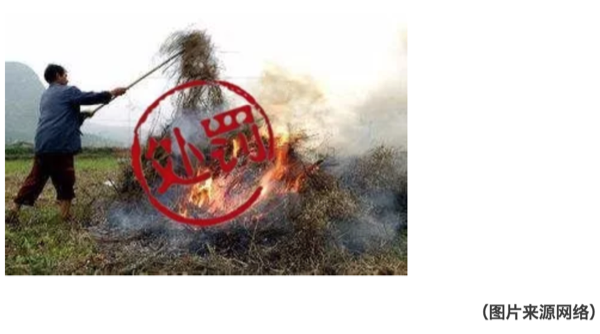
\includegraphics[width=8.33in]{images/stalk3}

为了彻底杜绝火点,在大气污染防治法的框架下,有些省份开出了自己的处罚清单。河南省在增加督查和暗访的基础上,以环保部公布的秸秆焚烧卫星监测火点数为依据,以县(市、区)为单位,出现一个火点,省财政扣拨县(市、区)财政资金50万元,力度之大空前绝后。

秸秆问题逐渐进入人们的视线并得到如此重视,除了它与雾霾之间千丝万缕的联系之外,还因为它的确是农业和环保领域牵一发而动全身的节点。

一根秸秆,一头连着三农,一个敏感脆弱又是万事之本的领域,一头连着环保,一个同样是成长痛点难点的行业。不能烧,但也不能接受粮食减产!粮食减产,根基没了,中国人民要挨饿;烧秸秆,污染加剧,人民叫苦连天。相信很多民生问题都是如此。

好在中国人民是世界上最勤快的人民。纵观其他国家,在面对这个问题的时候农民往往是两手一摊,对执法人员说``我没办法呀!''\ldots{}\ldots{}毫无悔改之意。

美国作为一个重要的粮食输出国,直到2011年在中部和东南部仍有大量火点发现,可比我国东北严重多了,有NASA图为证。印度人民更是开挂,烧着秸秆接受记者采访,大大方方毫不避讳。

秸秆的五料化利用技术(肥料化、饲料化、基料化、燃料化、原料化)并不高深,而秸秆问题的处理方式千差万别,对应效果天壤之别。

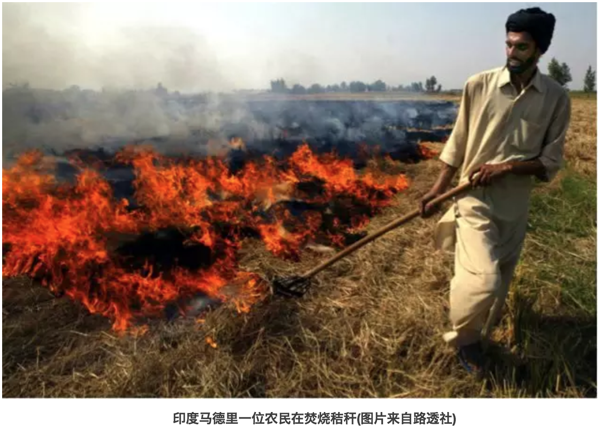
\includegraphics[width=8.33in]{images/stalk4}

解决秸秆问题,一个靠重视,一个靠财政。回看我国,重视程度和经济投入力度都需更进一步。

2007年,美国政府投资1.25亿美元建设了3个生物能源中心,专门进行纤维素生物能源研究。同年,美国农业部出资1400万美元、能源部出资400万美元,共同设立基金研发生物燃料、生物能源及相关产品的研究与开发。

据统计,2008-2012年,美国政府对生物质研发法中涉及的项目共计投资了1.18亿美元。除了对研发环节和支持外,美国对可再生能源发展规定了技术开发抵税和生产抵税的措施,生物质发电和秸秆纤维素乙醇项目都享受响应的税收补贴或者减免。

对比我国,2016年,农财两部门整合资金10亿元,选择秸秆焚烧问题较为突出的10个省份开展秸秆综合利用试点,取得了初步成效。果然真金见实效。

现在秸秆综合利用的主要方法是还田(直接和间接),直燃、气化、制沼,制醇和用作饲料、栽培基料等。

还田的方式简单、粗暴、直接、见效快,被各地采用最多,但由于地域差异明显,也存在一些弊端和后患。

直燃、气化、制沼和制醇等方式都需要大量的经费投入,各省由于财政状况难以统一,无法按照某个标准整体推进;另一方面,秸秆禁烧和综合利用与农户素质密切相关,在加大财政投入的同时,提高农民认识,增强回收利用秸秆的积极性也是较为有效的措施。

而在环境黑板报更新的《纳米非米》中,提出了以秸秆等有机废物为原料制备生物碳材料``以废制废''的观点,也是秸秆处理另一条可选择的路径。

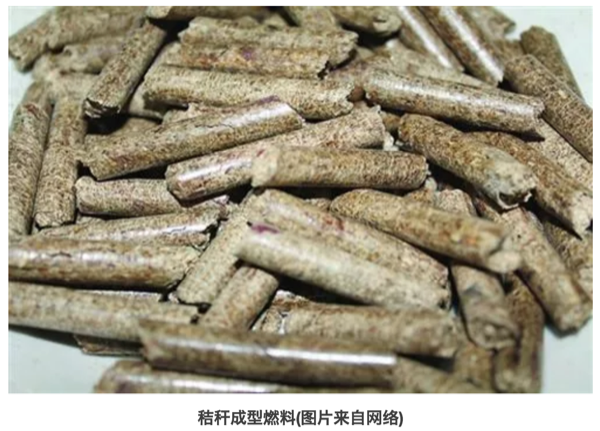
\includegraphics[width=8.33in]{images/stalk5}

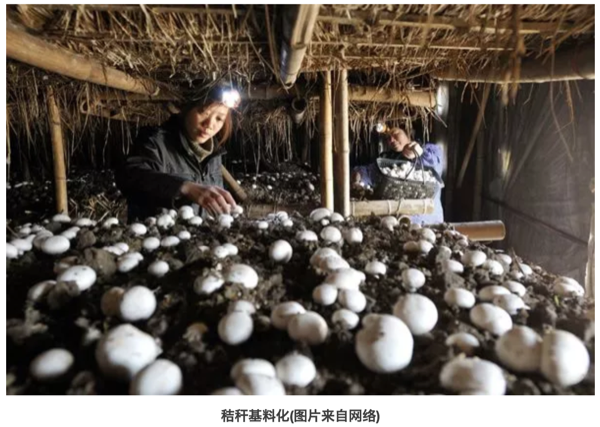
\includegraphics[width=8.33in]{images/stalk6}

\subsection{结语}

据悉,今年11月份哈尔滨火点问题爆出以后,相关责任人已于近日被环保部约谈,东北秸秆问题治理的机遇和挑战也随之而来。秸秆燃烧这种事,连遥感卫星都看得到,还怕执法部门不知道吗?小秸秆、大问题!希望所有的环保责任人能够直面问题,应对挑战。在关注大动向时,不忘记身边还有这样的``小事情''也同样需要我们的努力!

作者:胜利屯支书 校稿:广播站王站长、柴胡半夏苏 编辑:竹而乐

\section{VOC减排------大气治理的新挑战}\label{voc}

\subsection{前言}\label{-1}

``今天空气质量怎么样?适不适合户外活动?''关注空气质量已经成了人们日常生活的一部分。由于人口增长和工业及经济的快速发展,人类在生活和生产中向大气中排放的污染物量也日渐增多,主要包括二氧化硫、氮氧化物、烟粉尘等颗粒物、挥发性有机化合物(Volatile
organic
compounds,VOCs)等等,而由此引发的大气污染问题也层出不穷:除了被热议的灰霾,酸雨、温室效应、光化学烟雾、臭氧层破坏、有毒物质扩散等也不容小觑。随着《大气污染防治行动计划》的实施,我国对二氧化硫、氮氧化物、烟粉尘排放控制取得明显进展,但VOCs防治工作相对滞后。目前,VOCs减排已经成为大气污染防治的重点。VOCs是什么?对于局外人来说,可能非常陌生,但在大气治理的圈子内,它已经火的不要不要了。那么,挥发性有机物到底是何方神物,会引起如此大的关注?

\subsection{VOCs是何物}\label{vocs}

\subsubsection{VOCs的定义}\label{vocs}

学术界对于VOCs的定义是指沸点在50\textasciitilde{}260℃,室温下饱和蒸汽压超过133.32Pa的易挥发性有机化合物。简单点说,挥发性有机物首先是有机物,然后这种有机物容易由液态转为气态物质进入环境空气中。举个例子,装修完之后,很多朋友会关心甲醛的问题。甲醛是胶粘剂的主要成分,板材中残留的和未参与反应的甲醛会逐渐向周围环境释放,甲醛就是生活中最常见的VOC。除了甲醛,生活中接触到的油漆、汽油等都含有VOCs。

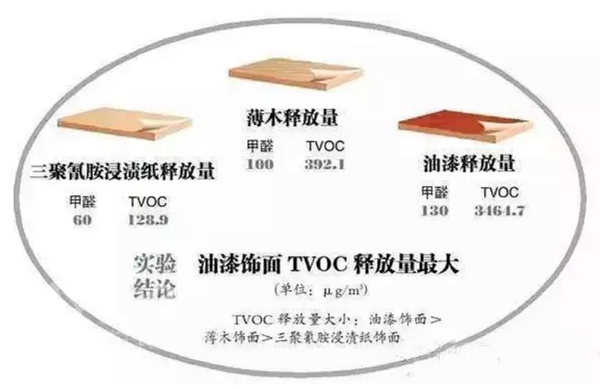
\includegraphics[width=8.33in]{images/voc1}

VOCs之所以被关注、被研究、被减排,就不得不说说它的危害。VOCs不仅危害环境,而且危害身体。一方面,VOCs是大气环境中光化学反应的前体,在阳光照射等特定条件下,会与环境空气中的化学物质,发生一系列光化学反应,生成臭氧,而形成光化学烟雾。同时,VOCs也是灰霾重要的前体物质,通过对细颗粒物(PM2.5)源解析,大气中VOCs在PM2.5中的比重占20\textasciitilde{}30\%,还有部分PM2.5由VOCs转化而来。

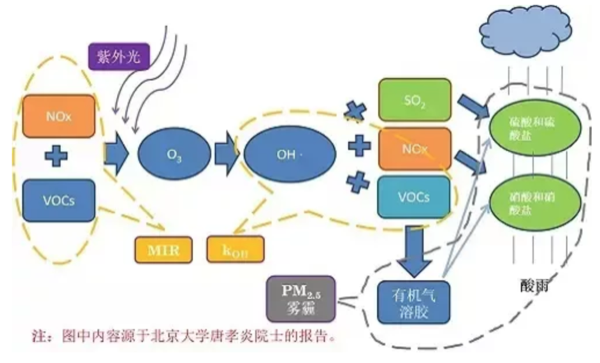
\includegraphics[width=8.33in]{images/voc2}

另一方面,大多数的挥发性有机物均有病理毒性,都对人体各器官组织有较大的危害作用。以甲醛为例,其在室内达到一定浓度,可引起眼红、眼痒、咽喉不适或疼痛等症状。

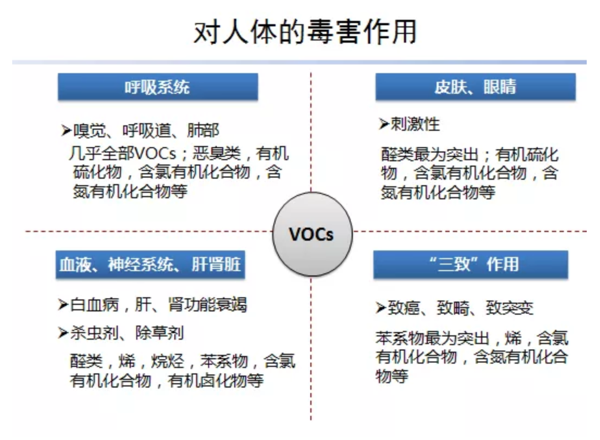
\includegraphics[width=8.33in]{images/voc3}

VOCs排放源主要包括自然源和人为源。自然源主要为植被排放、森林火灾、野生动物排放和湿地厌氧过程等,属自然界的正常规律,源和汇处于平衡状态。而人为源大致可分为工业源、生活源、农业源和移动源。有调查报道,我国VOCs的工业源和交通源为主要的人为源,分别占43\%和28\%。

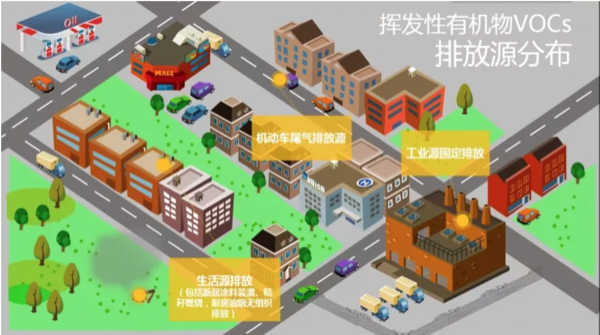
\includegraphics[width=8.33in]{images/voc4}

其中工业源排放企业涉及的行业有电子信息、纺织印染、石油化工、家具、木材加工、塑料橡胶制品加工、包装印刷、制药等,这些行业也正是目前我国主流工业。正因为人类活动,越来越多的VOCs进入大气中,在环境空气中的累积,打破了自然界VOCs源和汇的平衡。

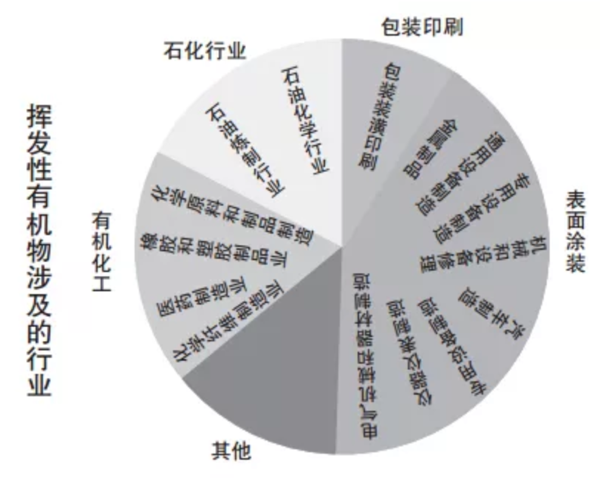
\includegraphics[width=8.33in]{images/voc5}

1940年至1960年间,美国洛杉矶多次发生光化学烟雾事件。在1952年12月的一次光化学烟雾事件中,洛杉矶市65岁以上的老人死亡400多人。1955年9月,由于大气污染和高温,短短两天之内,65岁以上的老人又死亡400余人,许多人出现眼睛痛、头痛、呼吸困难等症状甚至死亡。事件的主要原因是汽车尾气排放了大量的碳氢化合物,在阳光照射下,发生光化学反应,产生有毒气体。这是人类首次认识到VOCs的严重危害,因此,洛杉矶对VOCs的关注走在了世界的前列。1963年,美国以《清洁空气法》的规定为基本依据,要求卫生教育福利部处理空气污染问题,明确机动车对空气污染的影响,并通过环境保护署制定和颁布限值VOCs污染排放的一系列标准,指导全国执行VOCs排放限值。1970年7月,日本东京出现了光化学烟雾现象,几所大学连续出现学生眼睛疼痛、呕吐等现象。因此,日本在VOCs污染排放方面的关注也比较早。

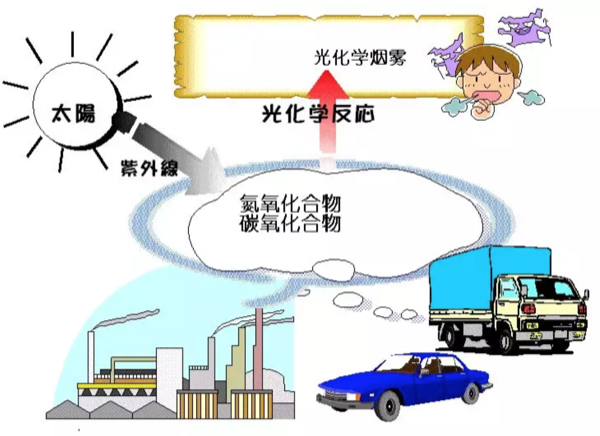
\includegraphics[width=8.33in]{images/voc6}

\subsection{VOCs的减排之路}\label{vocs}

\subsubsection{国家层面}

我国尚未出现过VOCs污染事件,因此对其关注较晚,2000年,《中华人民共和国大气污染防治法》中仅有诸如有机烃类尾气、恶臭气体、有毒有害气体、油烟等类似概念。

随着灰霾问题的深入研究和环境空气中臭氧浓度升高问题,VOCs逐渐被重视。为改善大气环境质量,促进VOCs削减,我国出台了一系列的政策。2013年,国务院出台《大气污染防治行动计划》,明确要对石化、有机化工、表面涂装、包装印刷等行业实施VOCs综合整治,全国范围内的VOCs减排正式启动。同年,环境保护部编制了《挥发性有机物(VOCs)污染防治技术政策》,为VOCs减排提供了技术规范支持。2015年8月29日第十二届全国人大常委会第十六次会议通过了《中华人民共和国大气污染防治法》,自2000年修订以来,首次增加对VOCs控制要求,从此VOCs减排有了法律依据。这些政策的颁布,从计划到技术、再到立法,逐渐指明我国VOCs减排方向。

在部门规章方面,国家发改委、环保部、财政部、工信部、质检总局、能源局等部委相继出台了有针对性的VOCs污染防治相关文件。各部门相互配合,共同打好VOCs减排攻坚战。

在技术标准方面,我国《大气污染物综合排放标准》(GB162972-1996)对14类VOCs规定了最高允许排放浓度、最高允许排放速率和无组织排放限值,其中包括甲醛、苯、甲苯、二甲苯等挥发性有机物。针对不同的有机污染物排放源以及污染源和环境空气中VOCs的监测技术,截止到2017年,环保部总共制订了15个涉及VOCs的排放标准和20个监测技术方法。从标准实施年限来看,2010年以前,只有3个排放标准和8个监测技术方法,其他都是近几年开始实施。技术标准的制定,为VOCs减排提供了监测和排放依据。

\subsubsection{地方层面}

为积极推动VOCs减排,各地结合地方实际,出台了一系列相关的政策法规和标准方法。表
1列举了北京和江苏省的VOCs污染防治政策。由表
1可见,我国地方从2010年前后,开始加强对VOCs进行管控。近一两年,VOCs污染防治成为各地大气防治的重点工作,各地不断完善VOCs减排政策措施。

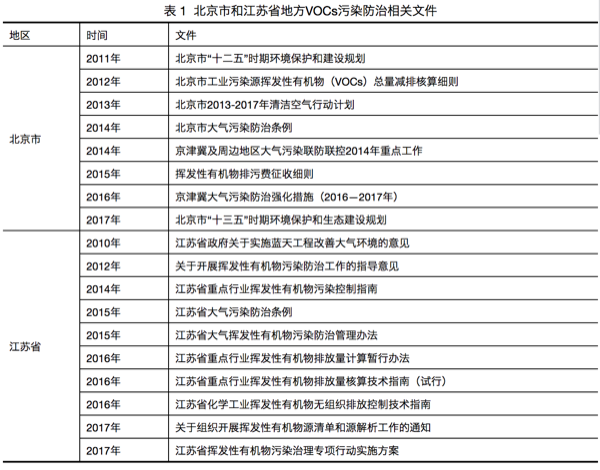
\includegraphics[width=8.33in]{images/voc7}

在技术标准方面,国内出台VOCs排放标准的省市并不多,以北京、江苏、浙江和广东为例,各地根据当地的产业特点,制定了相关VOCs排放标准。近两三年,北京连续制定了12项地方排放标准,涉及的行业有印刷、家具制造、炼油和石油化工、汽车、工业涂装和建筑涂料等;江苏重点针对化学工业和表面涂装行业,制定了相关地方排放标准;浙江以化学合成制药、制鞋、化学涂装、纺织染整行业为重点行业;广东以集装箱制造和电子行业为重点行业。

\subsection{VOCs减排技术和挑战}\label{vocs}

对VOCs减排的主要技术思路是源头控制和末端治理。简单的说,源头控制就是从原料开始,减少VOCs的产生。末端治理,顾名思义,将产生的VOCs进行最终的销毁。有两类基本技术,一类是回收技术,对排放的VOCs进行提纯处理,再资源化循环利用。主要包括吸收、吸附、冷凝和膜分离方法等技术。另一类是销毁技术,将排放的VOCs分解化合转化为其他无毒无害的物质。主要包括活性炭吸附、低温等离子、热力燃烧、催化燃烧等技术。

涉及VOCs排放的行业众多,污染物种类繁多,废气成分复杂,因此,在对VOCs减排时,要考虑技术上有效、经济上可行,往往这两者很难平衡,这也是VOCs减排面临的最大的挑战。

\subsection{小结}

因此,虽然我国对VOCs的管控起步较晚,为改善环境空气质量,近年来,我国已将VOCs减排作为一项重点工作,出台了相应的法律、法规、政策、技术规范等,并迅速形成一套体系,为VOCs污染防控指明了方向,提供了支撑和保障。

``大家非常关心中国会不会发生光化学烟雾事件,中国政府也高度关注。我们组织过专家分析,世界历史上发达国家发生的光化学烟雾一般臭氧浓度都达到了600以上,个别城市2000以上。中国的臭氧浓度远低于此,所以中国现在和将来不会、也极少可能会发生光化学烟雾事件。''引用环保部大气环境管理司司长刘炳江的一段话,作为总结,相信我国VOCs减排之路,对环境改善有重要的意义。

作者:远方老友 校稿:广播站王站长、柴胡半夏苏 编辑:栟

\section{等风来}

2000年左右,北京人讨厌风,因为一到大风季节,黄沙滚滚,遮天蔽日。可是近些年来,人们又盼着风,期望风来了,把自己从雾霾中解救出来,一时间``等风来''成了所有人的心声。雾霾和风几乎每年都会在北京的地界干上几场大仗,有时力量悬殊,战争迅速结束;有时势均力敌,展开拉锯战。下面我们详细解析一下双方斗争的形势。

\subsection{与雾霾的战争}

首先我们将北京全市PM2.5(细颗粒物)日平均浓度高于200微克/立方米、持续时间超过2小时的污染状况定义为一次重污染事件,2013年8月到2014年8月期间,我们共观察到六次重污染事件,分别为2013年10月28日(265.59微克/立方米)、2013年12月8日(202.63微克/立方米)、2014年1月23日(233.71微克/立方米)、2014年2月15日(437.15微克/立方米)、2014年2月26日(337.39微克/立方米)和2014年3月27日(234.32微克/立方米)。我们基于GIS软件,通过克里金差值方法对这六次重污染过程形成和消散过程进行了模拟。

\subsection{雾霾的胜利}

北京PM2.5重污染事件主要受外源传输影响。从重污染形成的过程看,北京这六次重污染过程中,细颗粒物从北京东南部或者南部,逐渐向城中心和西北部缓慢扩散,最终全城形成重污染(图1)。

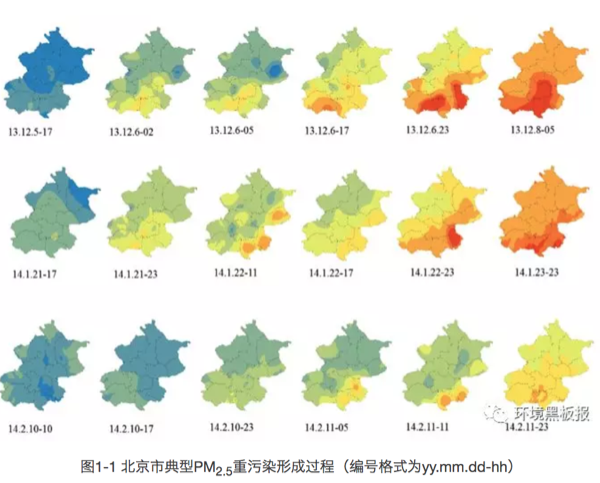
\includegraphics[width=8.33in]{images/windhaze1}

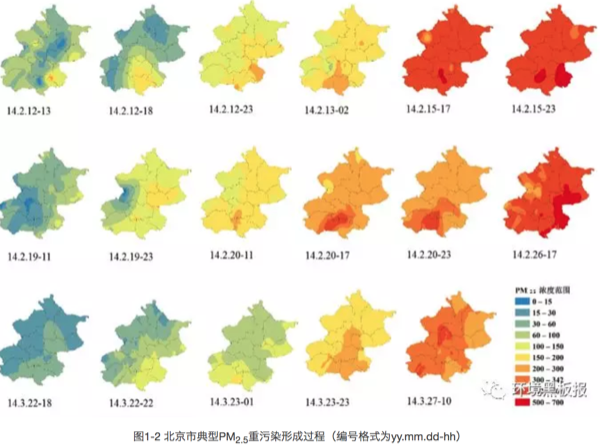
\includegraphics[width=8.33in]{images/windhaze2}

在重污染形成期间北京平均风速低于1米/秒,主导风向为南风和东南风(图2),说明北京的PM2.5重污染的形成受外源传输影响较大。主要的污染物来自北京东南部和南部的廊坊、天津和保定等省市。重污染的形成时间一般为3-7天。

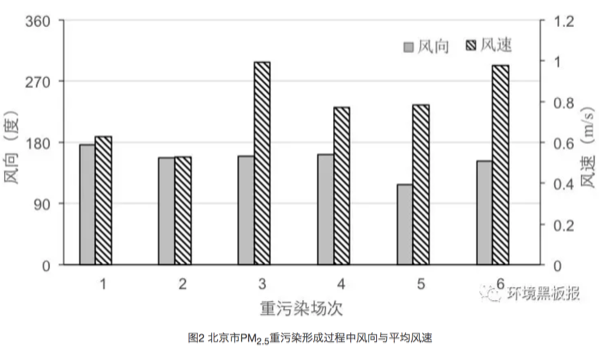
\includegraphics[width=8.33in]{images/windhaze3}

\subsection{大风的胜利}

北京PM2.5重污染的消散主要借助风。北京这六次重污染消散过程中,受风的影响,细颗粒物从北京西北部开始,逐渐向城中心和东南部推移,最终实现全城PM2.5消散(图3)。在此期间北京平均风速为2.5米/秒,而主导风向为西北风和北风为主,只有一次为南风。从模拟结果看,北京的细颗粒物被西北风一分为二,之后在向东北和西南逐渐扩散,直至完全消散。说明北京的PM2.5重污染的消散主要依赖于西北风的影响,而且平均风力为2.5米/秒(图4)。重污染的消散过程比较迅速,整个消散过程时间一般在6-11个小时,其中消散最快的一次,出现在2014年2月26日,全市平均PM2.5浓度从431微克/立方米降到21微克/立方米,仅用了6个小时,期间平均风速为3.2
米/秒,主导风向为西北风。其中最慢的一次(2014年2月17日)持续了18个小时。主导风向为东南风,风力2.4米/秒。可见,北京PM2.5的消散过程与风向和风力有密切关系。

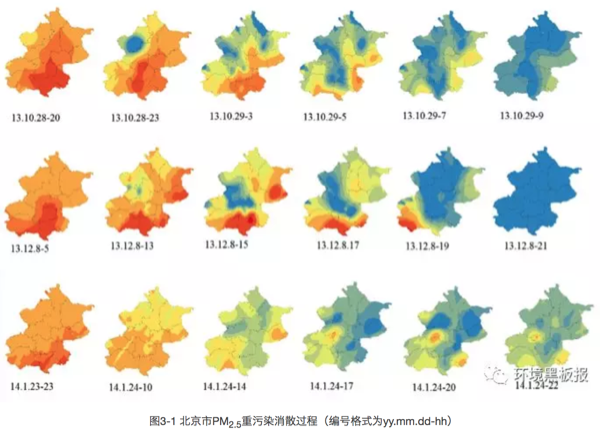
\includegraphics[width=8.33in]{images/windhaze4}

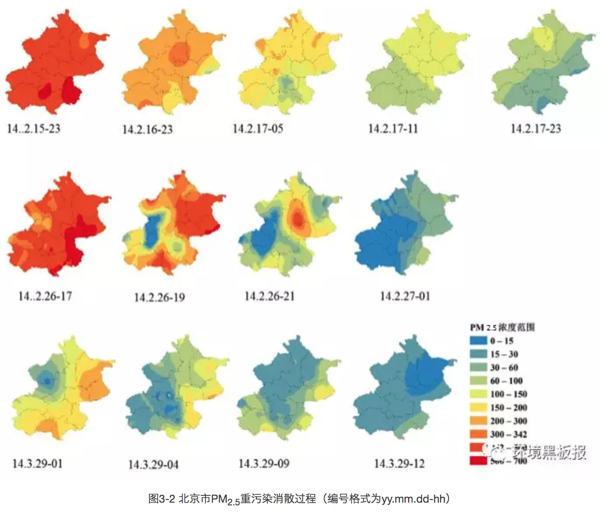
\includegraphics[width=8.33in]{images/windhaze5}

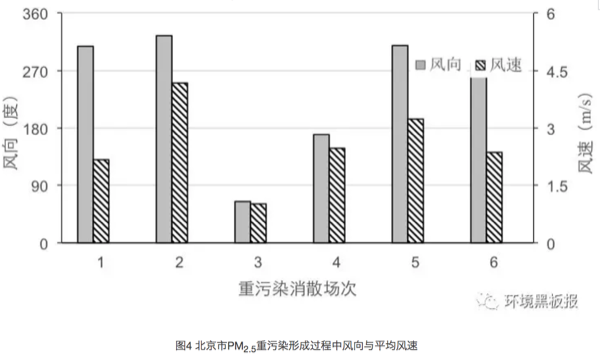
\includegraphics[width=8.33in]{images/windhaze6}

总体看来,风速1米/秒是一个坎,风速小于1米/秒,则容易形成雾霾累积;当风速大于1米/秒,重污染容易扩散,尤其是西北风。

\subsection{势均力敌}

2018年1月13-17日,京津冀及周边地区经历了一次大范围重污染过程,污染范围包括河北省、山西省、山东省和河南省等城市全部或者部分地区。石家庄市是受重污染影响较大的城市之一,截止到1月21日0时,本次中污染石家庄市出现了164个小时的重度污染和90个小时严重污染(数据来源于网络,未经审核)。

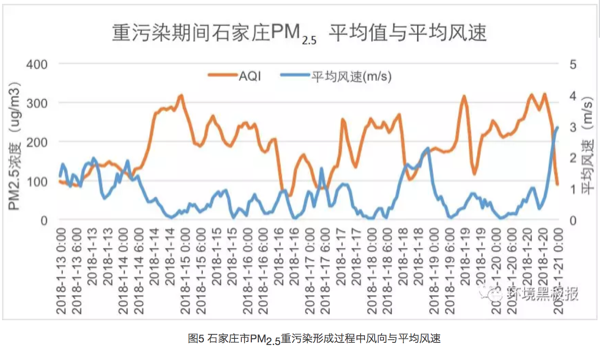
\includegraphics[width=8.33in]{images/windhaze7}

石家庄市从13日凌晨开始空气质量逐步转差,污染物浓度波动上升(图5)。13日5时达到重度污染,
14日6时,污染物逐渐累积,11时达到严重污染。16日14时至17日7时空气质量出现短时改善,部分时段降至中度污染以下水平。此后空气质量继续恶化,重污染持续,但污染程度轻于第一次累积过程。1月18日15时,再次得到短时缓解,之后污染物浓度继续升高,全市PM2.5小时平均值最高值出现在19日12时,达到317微克/立方米。之后迅速下降。1月19日16时,下降到最低值,为117微克/立方米。之后污染物继续累积,1月21日空气质量好转。截止到目前,重污染源已经持续393个小时,其中,有164个小时的重度污染和90个小时严重污染(数据来源于网络,未经审核)。

在此过程中,风速与空气污染指数呈现明显的负相关关系(图5)。风与霾此消彼长,在石家庄市展开拉锯战,持续时间已经超过一周。中间几次过程,主要风速大于1米/秒,空气污染就会得到改善。一旦面临静风时刻,污染物开始逐渐累积。

\subsection{雾霾攻坚---源头把控}

在污染治理上,我们要做的还有很多,默默的等风来,不是真正的解决问题的方法。根据贺克斌院士的观点,城市治霾的根本在于管住污染源。2017年8月18日《京津冀及周边地区2017-2018年秋冬季大气污染综合治理攻坚行动方案》(环大气〔2017〕110号)实施以来,在京津冀及周边地区2+26城市,坚持问题导向,把稳固``散乱污''企业及集群综合整治成果和高架源稳定达标排放作为坚守阵地,把压煤减排、提标改造、错峰生产作为主攻方向,把重污染天气妥善应对作为重要突破口,加强联防联控,严格执法监管,强化督察问责,全面实施攻坚行动,动员全民共同应对重污染天气。``攻坚行动''方案规定主要完成的11项任务中有8项与污染源管控有关。截止到2017年12月PM2.5浓度削减幅度最大的前六位城市是石家庄、北京、廊坊、保定、鹤壁和安阳市,与去年同期相比,PM2.5浓度削减幅度均在40\%以上,可见污染源管控才是真正解决雾霾的根本手段。

等风来不如去追风,幸福都是奋斗出来的,总有一天我们能切实做到污染源有效管控,从源头上减少排放,雾霾问题才能从根本上得到解决,相信我们生活的环境会越来越好。

作者:大石 校稿:看透,胜利屯屯长 编辑:丫头晚安

\chapter{工程实践}

\section{城市之殇}

\subsection{序言}

2012年7月21日,一场61年一遇的大暴雨让北京成为``汪洋水城'',想不到有生之年居然可以在帝都这个缺水的城市同时实现了``山盟海誓''。无独有偶,不仅北京遭遇了这样的窘境与困惑,其他城市诸如南京、武汉、广州、杭州等也先后开启了``看海模式'',这种``城市之殇''已经成为近年来城市发展挥之不去的阴影。

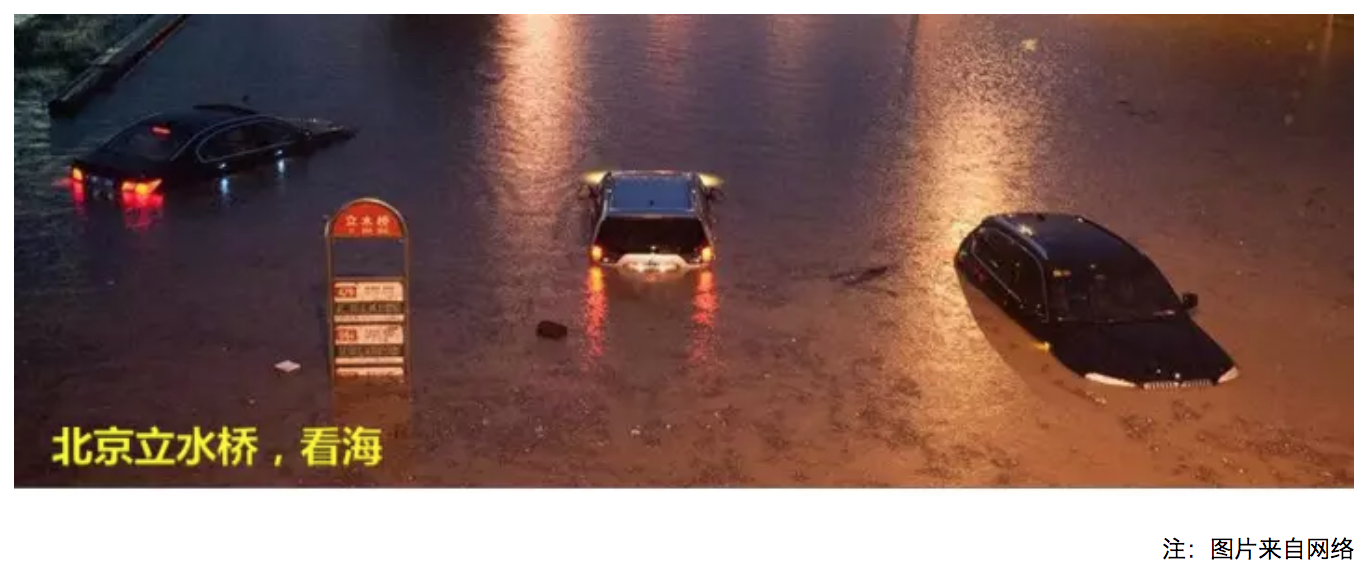
\includegraphics[width=6.67in]{images/ch1}

那么,为什么我们城市的排水能力一遇到暴雨甚至中小雨就原形毕露?这就有必要来聊一聊本期的话题:``海绵体''。海绵体,顾名思义,是一种对蓄水的形容,自然界原本是一个巨大的海绵体,而如今城市的爆发式发展建设已严重破坏了自然的海绵体,损害了自然的水循环系统。传统的城市建设模式根本不具备应对超标雨水的能力,那么必然会导致``逢雨必涝'',同时还会带来水环境污染、水资源紧缺、水安全缺乏保障等问题。

2013年12月12日,习近平总书记在《中央城镇化工作会议》的讲话中强调:``提升城市排水系统时要优先考虑把有限的雨水留下来,优先考虑更多利用自然力量排水,建设自然存积、自然渗透、自然净化的海绵城市''。海绵城市顺应时代号召应``运''而生。

\subsection{海绵城市是什么}

海绵城市的理念其实在我国古代早已践行,比如故宫的排水系统、云南的``哈尼梯田''模式、赣州的``福寿沟''蓄排系统等,都算作是早前的雏形。若要刨根求底地问海绵城市是什么,海绵城市更多的是一种新型的城市发展模式。

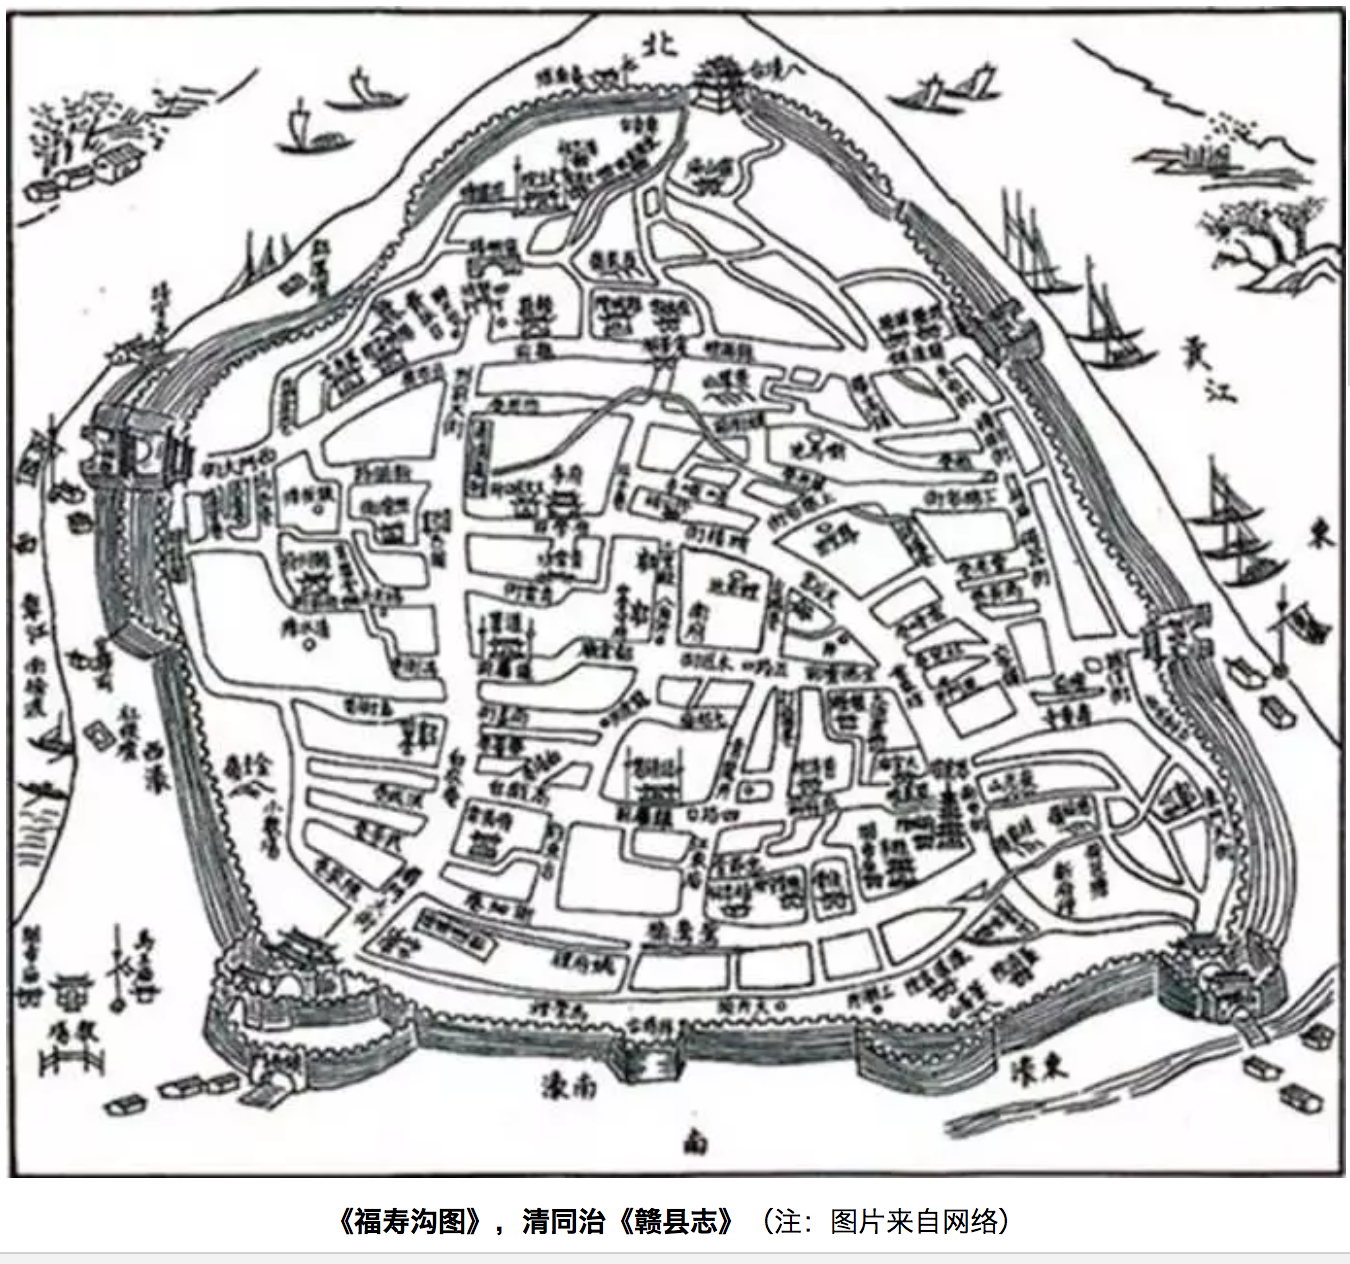
\includegraphics[width=6.67in]{images/ch2}

海绵城市的初衷是让城市能够像海绵一样,在适应环境变化和应对自然灾害等方面具有良好的``弹性''。简单来说,下雨的时候,城市可以像海绵一样吸水、蓄水、渗水,防止洪涝的出现;在雨水过后,干旱的时候,又可以将蓄存的水``释放''并加以利用。但同时,我们又希望这个``海绵''能发挥更大的作用,比如说还可以净化水体,让雨水在城市存积、渗透的同时得到净化,以利于进一步的雨水资源利用和生态环境保护。这就为海绵城市的设计、建设提出了更高的要求,不单是依靠恢复或构建自然途径来蓄水、存水,还应当结合人工措施来辅以完成水资源的净化、利用和排放。

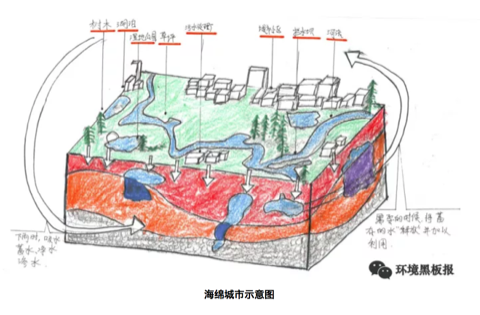
\includegraphics[width=6.67in]{images/ch3}

因此海绵城市的具体建设既不能``窄'',也不能``宽''。太窄就会回到植树造林搞绿化的老路子上去;太宽就会变成``海绵城市一个框,啥都可以往里装''。其实海绵城市建设还是要以目标与问题为导向,运用``源头、中途、末端''的措施,使绿色设施与灰色措施相结合,才能实现真正的目标。

简明地讲,源头主要以低影响开发设施(LID)为主,包括植草沟、雨水花园、生物滞留设施等,中途主要包括:雨水廊道、管网、沟渠等,末端主要包括:湿地、调蓄塘、调蓄池、水系等。

\includegraphics[width=6.67in]{images/ch4}

\subsection{海绵城市试点}

海绵城市的建设借助国家重视生态环境的东风,目前共执行了2个批次、30个城市的试点,试点期3年。期内国家将给予直辖市每年6亿专项补助,省会城市每年5亿,其他城市每年4亿元。

\includegraphics[width=6.67in]{images/ch5}

\includegraphics[width=6.67in]{images/ch6}

目前来看,海绵城市建设还没有一个全国性的``统一标准'',主要是因为我国地域差异大,东西南北中,面临的问题与挑战各不相同。比如北方地区多为缺水的寒带地区,南方地区则更容易发生内涝,西部地区多属于湿陷性黄土地区,也极度缺水。因此不同区域的海绵城市建设也应因地制宜。

\subsection{浅谈海绵感悟}

笔者从2015年开始从事海绵城市建设方面的工作,先后参与了多地的海绵城市试点建设的咨询、设计等工作,主要涉及海绵城市建设系统方案编制等方面。这里跟大家分享一下三年多来笔者对海绵城市建设的一些想法与感悟,希望能对现在或将来参与到海绵城市建设中的同仁们有所帮助。

\subsubsection{从管理部门的角度}

如果您是一位相关部门的负责人,笔者虽人微言轻,但也愿意提供一些思考供您参考。
海绵城市的建设是一个很复杂、庞大、时间跨度也大的系统工程。而且里面涉及到很多学科和部门,简单数数就需要规划、市政、园林、水利、道路等专业;住建、水利、园林、环保等部门来互相配合。因此如何统筹规划,通力协作,避免形成各自为政、``九龙治水''的局面,是一门很深的学问。

同时,很多城市现在都有新、老城区,新城区建设制约少、阻力小,一旦方案设计得当,大可一马平川。但是老城区就不一样了,不仅居民多、遗留矛盾和问题多多,牵一发而动全身,搞不好容易激化矛盾。这个时候,就不能只顾海绵城市建设的目标,还要考虑经济承受能力、轻重缓急、资金利用效率、建设时序、社会影响等方面。
千万、千万不能不分轻重地全面开工建设和盲目翻挖。最好可以以解决城市内涝、雨水利用、黑臭治理为突破口,结合棚户区和城乡危房改造、老旧小区有机更新等工作同步推进。

\subsubsection{从项目公司负责人的角度}

当前海绵城市的建设基本上都以项目打包的形式交由PPP公司全权负责建设。如果您是一位项目公司的负责人,首先恭喜您拿下了海绵城市的项目,但是接着愁人的事情来了。在很多项目管理过程中,一些PPP公司``当家不做主'',没有自主权,项目的管控不是由PPP公司独立操作,而会受到相关部门的干预,导致指挥不合理的局面。因此,如果您能在项目开展前和相关部门做好充分的沟通,对您后续工作的开展会有很大帮助。
同时,虽然目前海绵城市都处在建设之中,但是即使这样,试点期也已经过了2-3年,后期的运营维护也该做一些考虑了。如果您公司还没有做这方面的准备,那可千万要小心了,现在环境追责可是很严重的哦。

\subsubsection{从设计师的角度}

如果您是一名规划师或者设计师,请一定要``迈开腿,管好嘴''。一定要多去现场,没有调查就没有发言权,不能板凳一坐就站不起身,嘴皮一碰就出方案。曾经有一位设计院的设计师理直气壮地反驳说没必要去现场看这么细,走了个过场回来,后来设计的时候全部依靠业主来提供信息作为依据。结果可想而知,做出来的设计方案根本经不起推敲,漏洞百出,更别说拿去指导施工建设。

\includegraphics[width=6.67in]{images/ch7}

同时也提醒大家,海绵城市建设不只是``搞种植、搞绿化''。``花花草草''固然重要,但我们也不能天天搞``拈花惹草''的老一套。海绵城市的实质应该是绿色设施(雨水花园,植草沟,下凹式绿地等)与灰色设施(管网,泵站,调蓄池等)相结合,让它们在不同时间与空间上起到相应的功能与作用。

\subsection{结语}\label{-1}

海绵城市的概念一经提出,就在全国迅速地铺展开来。国内新事物的出现,不像国外``自下而上''的推进模式,而是``自上而下''的运动式推动。然而,没有前期多年的研究数据作为支撑,直接开展工程实践难免会面临各种各样的困境。
目前,``海绵城市''的提法基本已家喻户晓,无人不谈``海绵'';然而能真正潜下心来认真对海绵城市进行系统的研究与梳理的人却少之又少。一个新的领域,往往需要十年甚至更长的时间来形成系统性的理论与技术体系,之后才有可能更高效、更全面指导工程实践。希望各位海绵同仁,我们一起潜心努力,为这个领域尽自己的绵薄之力。

作者:王宇 校稿:广播站王站长 编辑:栟 手绘美图:丫头晚安

\section{污师私房菜之OUR 和 SV30 的应用}\label{our--sv30-}

在污水处理领域,活性污泥工艺可谓无人不知无人不晓。活性污泥吃着排泄物,干着体力活,最终为我们产出清水,真乃当下``撸起袖子''的楷模。说到活性污泥真是让人既爱又恨,爱的是它能帮我们处理污水,恨的是它不善于表达,和人类语言识别系统无法链接,当污水处理系统出问题的时候,初入运维界的你却无法第一时间判断活性污泥究竟为什么罢工,只能求爷爷告奶奶的到处请教大神。

\includegraphics[width=6.67in]{images/os1}

今天通过\textbf{活性污泥呼吸图谱}和\textbf{污泥沉降性比}的应用介绍,通过熟练掌握这两个污水处理厂运维秘籍,让你可以和活性污泥随时交流,对污水处理厂的运行维护清晰把脉,及时准确解决出现的问题,让你的格调得到迅速提升,变身污水处理领域的运维大神。

\subsection{呼吸速率的前世今生}

话说20世纪50-70年代,国外有一群水处理界的大神(Eckenfelder,Mckinny,Lawrence-McCarty)闲着没事东看看西瞅瞅,就弄了个活性污泥模型出来,在里面就提到了\textbf{呼吸速率}(Oxygen
Uptake Rate,
OUR)的概念。所谓\textbf{呼吸速率是指单位时间内活性污泥消耗的溶解氧的量}。呼吸速率的概念由来已久,关于测量呼吸速率的专利也是层出不穷。然而呼吸速率一直应用于模型理论层面,在实际指导污水厂的运行方面却是凤毛麟角。(如何测量OUR就不在这里赘述了,请大家自行查阅相关秘籍)

我们知道在活性污泥工艺中有两种主导微生物:异养微生物和自养微生物。\textbf{异养微生物}需要消耗外部碳源维持自身生长(不给肉吃,它就死给你看);而\textbf{自养微生物}就是楷模了,可以通过分解无机物获得能量维持自身生长(真是吃着土,干着活)。这两种微生物都有各自的呼吸速率,异养微生物降解有机物时的呼吸速率称为\textbf{异养菌呼吸速率};自养微生物降解氨氮时的呼吸速率称为\textbf{自养菌呼吸速率}。有时活性污泥闲着无事也会吃些自己身上的东西,把微生物利用细胞内含物质作为基质进行新陈代谢过程中的呼吸作用称为\textbf{内源呼吸速率}。图谱如下图所示:

\includegraphics[width=6.67in]{images/os2}

\subsection{OUR应用的理论介绍}\label{our}

上面介绍了呼吸图谱的组成,下面来谈一谈呼吸图谱的作用。为了更清楚的起到对比,我们需要在污水处理厂正常运行时,刻苦用心的你日常闲来无事多测测好氧池OUR,建立一个污水处理厂的OUR数据库,对正常情况下的OUR烂熟于心,只有这样你才能了解你自己一亩三分地的情况。

通常,\textbf{活性污泥OUR值的大小及其变化趋势可对好氧池负荷的变化情况起到预警作用,同时OUR的变化也间接反映出活性污泥自身的健康情况}。我们分两类情况进行分析:

\subsubsection{OUR异常高于正常值的情况}\label{our}

如果OUR若大大高于正常值,表示活性污泥需要消耗大量的溶解氧,表明优秀的活性污泥小伙子们正在撸起袖子加油干,这也往往预示着污泥负荷过高,可能超过污水处理厂的处理能力,这时出水水质可能超标。

\begin{quote}
你可以脑补一下这个场景:一个房间里面有十个饥饿的小伙子,你拿来十个馒头,他们能以迅雷不及掩耳盗铃响叮当之势把这十个馒头干掉,可如果你拿来一千个馒头,就算是吃到怀疑人生也吃不完。
\end{quote}

\subsubsection{OUR异常低于正常值的情况}\label{our}

如果OUR长期低于正常值,表示活性污泥消耗的溶解氧较少。这就需要分两种情况来分析了,一种情况是活性污泥精神抖擞,战斗力强,污染物负荷较小,污染物降解好,出水水质好;另外一种情况就是污泥活性差,污泥本身对污染物的降解性能不良,这可导致出水水质不达标。

\begin{quote}
第一种场景是这样的:一个房间里面有十个饥饿的小伙子,你就给五个馒头,估计最后盘子都会被吃掉;
\end{quote}

\begin{quote}
第二种情况是这样的:同样是这个房间,同样是五个馒头,但是吃馒头的人变成了十个胃口欠佳的病人,结果可想而知。
\end{quote}

\subsection{OUR应用的实战演练}\label{our}

上面对OUR应用的理论介绍还是比较笼统的,下面详细讲解一下如何利用OUR来判断出水水质,针对OUR的应用进行实战演练。

\subsubsection{实战场景1}\label{1}

用心的你费了九牛二虎之力测定了好氧池的OUR,发现OUR值比较低,根据理论分析,你记住了OUR异常低于正常值的第一种分析情况,认为活性污泥小伙子们战斗力强,降解能力个顶个,赶紧跟领导汇报说出水达标没有问题。你刚汇报完,厂里就通知你出水超标了,这脸被打的啪啪响。

这时,你一定会问,OUR值低,说明出水水质好,怎么出水还超标了呢。少年不要急,听我慢慢说来。

在OUR值比较低的情况下出水超标,说明此时的活性污泥并没有正常工作,那该如何解决呢?这种情况下你只需要往装置内部补充\textbf{足够的碳源},最常见的是投加乙酸钠,看看\textbf{投加碳源后的OUR值变化},如果OUR值还是很低,说明你的活性污泥活性差,大多都是老弱病残,再怎么给他们喂食碳源也不能发挥他们的作用;如果OUR值在投加碳源后明显升高,说明你的活性污泥是健康的,他们只不过是饿了,需要饱食一顿接着好好干活。

\textbf{因此,在好氧池OUR值比较低的情况下,判断出水是否达标的时候,需要结合好氧池当下的OUR和投加完碳源后的OUR进行判断,才能准确对污水处理厂的运行状态进行评价。}

\subsubsection{实战场景2}\label{2}

勤快的你这天又测定了好氧池OUR,发现OUR值很高,结合OUR异常高于正常值的情况分析,你下结论说出水水质达标。

少年你又要被打脸了。

\textbf{好氧池当下OUR值高,说明好氧池中污染物负荷高,表明好氧池需要消耗大量的溶解氧,为了保证出水达标,你需要做一系列应对措施,比如增加曝气,减少排泥量等等,只有这样才能保证你的出水达标。}

\subsubsection{实战场景3}\label{3}

就是这么巧,你们公司属于水处理界佼佼者,你一亩三分地里面管辖着若干个污水处理厂,你也坚持着建立了各个污水处理厂OUR的数据库,你也是一个闲着无聊喜欢翻数据的人。有一天,你发现针对不同污水处理厂,即使在进水和出水水质相差不大的情况下,好氧池的OUR差别仍然很大,这时你又迷茫了。

不要迷茫少年,因为在测量OUR时并没有考虑\textbf{污泥浓度}的因素,\textbf{污泥浓度高的,表明污泥中活性微生物较多,OUR值较高,污泥浓度低的,表明活性微生物少,OUR自然就低一些}。你可以想象一下,10个人和100个人的体重还是有很大差别的。

那如何采用一个统一的评价指标来评价呢?我们在污水处理厂的运营维护过程中,善于发现问题的同时,还要善于解决问题。这时,我们引入一个叫\textbf{比呼吸速率}(OUR/MLSS)的评价指标,你就会发现在入水水质和出水水质相差不大时,各个水厂的比呼吸速率相差也不是很大,是不是完美的解决了你的困惑呢?

\subsection{SV30的应用实战}\label{sv30}

上面给大家讲了比较高大上的OUR,接下来再给大家讲讲污泥沉降比的实战应用。SV30,在污水处理界的地位,犹如《天龙八部》中的扫地僧。可谓是量筒在手,天下我有。

做过污水处理的人应该都知道,\textbf{污泥30min沉降性能},可以一定程度上说明污泥的性状,所谓画虎画皮难画骨,具体判断污泥处在哪个状态却不是一件容易的事。可能或许也许maybe只有真正达到扫地僧的级别才能通过SV30一眼识别出污泥的性状来。

少年也不必灰心,鄙人在藏经阁翻阅典籍无数,浏览宝典若干,给大家总结了一些关于SV30的要点。大家理论联系实际,在测试SV30的时候,通过实际观察并结合我提供给大家的要点,相信大家早晚能达到扫地僧的级别。

\includegraphics[width=6.67in]{images/os3}

这里告诉大家一个小诀窍,千万别告诉其他人。

在测试SV30的过程中,重点观察\textbf{前5min的沉降效果},活性污泥沉降实验的前5min往往可以完成沉降过程的80\%,此阶段的沉降效果好坏往往可以指导对活性污泥性能的判断。

你可千万别取完样定个时间,先睡他半小时。所谓武功再高也怕菜刀,在测SV30的时候\textbf{量筒的选择}很重要,建议大家选用1L的量筒,量筒过小可能会发生污泥挂壁现象影响效果。再次重申,这些小诀窍千万别告诉其他人哟。

\subsection{结语}\label{-2}

以上算是给大家介绍了关于污水处理的两个秘籍,

一个是修炼较困难的葵花宝典------OUR,

一个是老少皆宜的太极拳------SV30。

所谓难易结合才能事半功倍。当然,掌握了以上两个技能也不能洋洋自得,天下之大,无奇不有,只有不断充实自我,才能屹立在污水处理行业的尖端。

\includegraphics[width=6.67in]{images/os4}

作为一个21世纪的污水厂操作人员,作为一个生活在大数据、物联网、云计算时代的污水厂操作人员,作为一个人工智能正在逐渐取代你饭碗的污水操作人员,仅仅依靠设计规范上面的知识已经难以追上时代的列车了。只有与时俱进,汲取新知识,用知识的力量将命运牢牢把握在自己手里。

成神的道路注定是孤寂乏味的,成神的道路注定是披荆斩棘的,成神的道路注定是一往无前的。少年,抓住当下,紧跟大师步伐,成神指日可待。

作者:阿布呆 校稿:看透, yufree 编辑:智公子 美图:丫头晚安,智公子

\section{纳米非米}

随着``水十条''、``气十条''和``土十条''的出台,我国已全面启动了``向污染宣战''的环境大战。那么纳米材料如何在环保领域掀起新潮呢?本文以碳纳米材料为一个视角,从选料-制备-应用的角度浅谈一下纳米材料在环保领域如何小试牛刀。

\subsection{碳纳米材料}

相信在很多读者的印象中,``纳米(Nanometer)''一词总是披着神秘的面纱,影影绰绰,忽远忽近。那么纳米到底是什么?实际上,它与毫米、厘米和分米一样,也就是个长度单位而已,十亿分之一米,即一纳米。

纳米尺度的物质在性质上,跟宏观物体表现出巨大的差异。比如纳米级的金子不再是金色而会失去光泽呈现黑色,纳米级的导电体会变得绝缘,坚硬的金属在纳米级会变得柔软。实际上,无论是人工纳米材料还是天然纳米材料,我们经常与它们亲密接触。大家几乎天天使用的数码电子产品的中央处理器就是用纳米材料制备;iphone的疏油涂层、国家大剧院的穹顶都与纳米材料有关;军事里的隐形战机也是涂了一层吸波纳米材料;甚至大气里的雾霾也包含了各种尺寸的纳米颗粒。可以说纳米材料已经与我们的生活息息相关了。

碳纳米材料的重要性和应用潜力已在最近20年的最高科学奖项中得到承认,包括1996年诺贝尔化学奖(富勒烯)、2008年卡弗里奖(碳纳米管)和2010年诺贝尔物理学奖(石墨烯)。由于其独特的理化性质,碳纳米材料在环境治理领域的应用研究一直是热点之一。然而由于目前的碳纳米材料制备方法成本高、产率低、条件苛刻、生产过程会伴有有毒副产物,极大地限制了其在环境领域的实际应用。因此,迫切需要开发高效、绿色、低成本的材料制备技术。在此背景下,该领域里近年来兴起的``以废治废''新概念逐渐引起了注意。意即将人们通常视作废弃物的材料(如富碳生物质)加工处理成碳材料,再投入到环保相关领域里使用。

\includegraphics[width=8.33in]{images/nano1}

\subsection{哪些废弃物可以加工成纳米碳材料?}

一般来讲,可以加工成纳米碳材料的废弃物,可以按其环境价值分为两类。一是低值类废弃物。如秸秆、稻草、稻壳等植物类废弃物;动物粪便、剩余污泥等有机质废弃物;以及甘蔗渣、甜菜渣等工业废弃物;二是负值类废弃物,如塑料袋、塑料瓶、海绵、轮胎等。

这两类的大多数废弃物都未得到合理利用,以此类废弃物作为原料制备碳纳米材料,一方面可以降低大规模生产时的成本,另一方面也可解决传统处置方式可能引起的环境污染问题。例如我国农村地区的秸秆(环境黑板报后续会有关于农村秸秆的专题文章)和农膜问题,大量焚烧会造成严重的空气污染和资源浪费。

\includegraphics[width=8.33in]{images/nano2}

\subsection{如何将废弃物加工成纳米碳材料?}

一般有水热碳化法和直接碳化法。

水热碳化法是指在密闭环境中,以水溶液为介质,使原料在高温(100-300°C)高压下经过一系列复杂反应生成碳材料的过程(实际上就是将原料洗好、称好,放铁罐子里扔烘箱里反应半天左右就行)。用水热碳化法制备碳材料,因其操作简单、无污染、对仪器要求低、转化率高等优点被广泛应用。此外,水热法合成的碳材料表面通常会含有丰富的官能团,特别有利于其应用在工业废水的处理中。目前,包括木屑、树叶、稻壳、松针、塑料袋、废报纸等废弃物都被成功地通过水热法碳化成碳材料,还有研究通过此法成功地将草变成了荧光碳量子点。

直接碳化法是指将原料置于无氧条件(惰性气体)下,高温(\textgreater{}600°C)裂解成碳材料的过程。(实际上也很简单,就是将原料放到管式炉中通氮气或者氩气加热一段时间就可以)在高温条件下,原料中的挥发性有机物会逐渐被分解直至留下碳骨架。通常,直接碳化法还需加入一些化学活化剂或者氧化性气体来活化碳材料,以使其表面孔隙度和比表面积增强。碳化温度、升温速率、碳化时间等因素都会影响碳材料最终的形貌和性质。用此法合成的碳材料,表面会具有较强的疏水性,所以对有机污染物的吸附能力很强。

\subsection{纳米碳材料在环保领域有哪些用处?}

\begin{enumerate}
\def\labelenumi{\arabic{enumi}.}
\tightlist
\item
  土壤修复
\end{enumerate}

以废弃生物质制得的碳材料具有发达的孔隙结构,当被添加到土壤中时,可以明显改善土壤结构,降低土壤的体积质量\href{陈心想,耿增超。西北农林科技大学学报(自然科学版),2013,41:\%20167-174.}{1}。另外,生物质以生物质碳材料的形式贮存在土壤中,C元素被固定,减少了向大气的排放;另一方面,生物质碳材料也可以为土壤提供N等营养元素,提升土壤肥力\href{Kezhen\%20Qian,\%20Ajay\%20Kumar,\%20et.al.\%20Renew.\%20and\%20Sustain.\%20Energy\%20Reviews,\%202015,\%2042:\%201055-1064.}{2}。上海交大曹心德教授认为生物质碳材料还可以用于土壤污染物的稳定化修复,他将具有独特吸附性能的碳材料形象比喻为``吸盘'',对土壤中重金属和有机污染物进行吸附``封锁'',从而阻碍植物对污染物的吸收。Puga
A. P.等人将甘蔗秸秆制成碳材料用于土壤中重金属钝化研究,发现其可将Cd、Pb
和 Zn 的有效态分别降低 56\%、50\% 和
54\%,并抑制它们向地上部的迁移\href{Puga\%20A\%20P,\%20Abreu\%20C\%20A,\%20et\%20al.\%20J.\%20of\%20Environ.\%20Manage.,\%202015,\%20159:\%2086–93.}{3}。Khan.
S.等人使用盆栽试验研究证实,
用污泥制得的碳材料能够减少水稻对As、Co、Cr、Cu、Ni、Pb的吸收\href{Khan\%20S,\%20Cai\%20Chao,\%20et\%20al.\%20Environ.\%20Sci.\%20\&\%20Technol.,\%202013,\%2047\%20:\%208624-8632.}{4}。当然,不同的废弃物原材料、碳化温度、碳化方法制得的碳材料物理化学性质不同,其土壤修复的效果也有差异。

\begin{enumerate}
\def\labelenumi{\arabic{enumi}.}
\setcounter{enumi}{1}
\tightlist
\item
  污水处理
\end{enumerate}

废水中常见的污染物有重金属离子、染料及其他有机污染物。吸附法处理废水由于工艺简单、成本较低、可利用吸附剂来源广泛等优势倍受青睐。废弃物加工制得的碳材料比表面积大、孔隙度高、表面基团丰富,对吸附废水中的污染物十分有利。研究表明,以废弃物为原料制得的碳材料不仅可以通过表面作用(静电吸引、疏水作用、π-π作用等)对重金属离子和有机物分子进行吸附(adsorption),还能凭借较高的孔隙度对油类污染物进行吸收(absorption)。例如新加坡南阳理工大学张华教授课题组成功将废报纸制得碳气溶胶材料用于油类物质和有机溶剂如氯仿等的去除,取得了较好的处理效果\href{Bi\%20H,\%20Huang\%20X,\%20et\%20al.\%20Small\%202014,\%2010,\%203544.}{5},这为解决海洋原油泄露污染提供了一个潜在的解决思路。印度理工学院鲁尔基分校Vinod
K.教授将废轮胎制得的碳材料作为吸附剂处理水中重金属离子,发现其对Pb2+、Ni2+有非常好的吸附能力\href{Gupta\%20V\%20K,\%20Ganjali\%20M\%20R,\%20et\%20al.\%20Chemical\%20Engineering\%20Journal,\%202012,\%20197:\%20330.}{6}。陕西师范大学张志琪教授课题组成功将香蕉皮碳化为多空碳材料,发现其对水中典型染料分子亚甲基蓝有较好的吸附去除能力\href{Liu\%20R\%20L,\%20Liu\%20Y,\%20et\%20al.\%20Bioresourse\%20Technology\%202014,\%20154:\%20138.}{7}。

\begin{enumerate}
\def\labelenumi{\arabic{enumi}.}
\setcounter{enumi}{2}
\tightlist
\item
  能源应用
\end{enumerate}

此种碳材料由于较高的石墨化程度,其电子传递能力较强。又由于生物质中还有大量的N,P,S等杂原子,使得由其制备的碳材料导电性进一步增强。因此此种材料在电化学上也具有广阔的应用前景。例如碳材料因为比表面积大、稳定性好、导电性好、价格便宜、来源丰富而成为超级电容器电极材料的首选。我们日常生活中的新能源汽车、数码相机,甚至楼道应急灯都有超级电容器的身影。例如大连理工大学邱介山教授课题组将虾皮制备成氮掺杂碳材料用作超级电容器,其在电流密度为50
mA/g时,比电容可达357
F/g\href{Gao\%20F,Qu\%20J\%20Y,\%20et\%20al.\%20Electrochim.\%20Acta\%202016,\%20190:\%201134.}{8}。利用西瓜皮、麦秸、绿茶、柚子皮、稻壳等制成的碳材料也可作为性能优异的负极材料用于锂离子电池。例如新加坡南洋理工大学于霆教授将竹筷碳化成碳纤维用于锂离子电池,其首次放电和充电质量比容量值分别为500mAh/g和283
mAh/g,且循环稳定性较好,有望替代传统石墨电极在锂电池中的作用\href{Jiang\%20J,\%20Zhu\%20J\%20H,\%20et\%20al.\%20Energy\%20Environ.\%20Sci.\%202014,\%207:\%202670.}{9}。

\includegraphics[width=8.33in]{images/nano3}

\subsection{结语}\label{-3}

以废弃物为原料制备的碳材料已被广泛研究用于土壤修复、污水处理和电化学领域,展现出了广阔的潜在应用前景。废弃物来源广泛、价格低廉的性质也使得此概念为大规模商业生产提供可能。然而目前对废弃物碳材料的研究才刚刚起步,处于发展阶段,很多碳材料仅限于实验室制备而没有进行大规模的工业化生产,距离大规模实际应用还为时尚早。

此外,在大规模应用之前,其对环境可能造成的潜在风险也有待进一步研究。这也正是纳米科技目前的发展缩影。正如中国科学院院长白春礼所说:``纳米科技发展方兴未艾,基础科学研究领域中新原理不断建立、新功能材料的涌现与可控制备技术的发展、纳米生物医药的应用探索都体现出纳米科技对人类知识体系的极大拓展以及对生活方式的潜在推动作用。尽管纳米材料显示了产业化以及临床应用的巨大前景,但多数材料目前仍处于实验室研究阶段,如何实现这些材料的功能化、推动商业化应用、相关的生态影响和生物效应是纳米科技发展面临的关键问题''。中国科学院生态环境研究中心江桂斌院士曾将基础研究形象比作翻书:``当书本一页一页翻至最后时,就是量变到质变的时候''。这也同样适用于纳米领域,或许质变之时我们就能用上充电几秒即可充满的电子产品,纳米机器人实现药物精准输送、有的放矢。

文献引用

作者:眼神防守 校稿:柴胡半夏苏,yufree 编辑:栟

\chapter{岸芷汀兰}

\section{念念不忘 必有回响}\label{-}

\textbf{广播站王站长}

行走在市区的环路上,穿插于市郊的街巷间,随处可见十九大的最新标语:``不忘初心,牢记使命''。环路上,有车水马龙的喧嚣;街巷间,有贩夫走卒的吆喊。初秋的北京,雄心壮志也很难抵挡供暖前的寒冷。在这座底蕴深厚、庄重方正复又灯红酒绿的都市里,每天面对拥挤的人潮和日复一日的生活,我常常会扪心自问:``究竟何为初心?''

初心常常不语。

要说来,环境专业其实是一个偏于冷门的小专业,在我刚上大学那会,环境学院一届就两个班,五十几号人;上研究生的时候一届也不到一百个学生。这么小的学院,如果非要说有什么优势,那就是女生比男生多,而且质量还不错。读博期间,那些二十七八岁,脱去白大褂立刻成为泪朱砂的妙龄女博士们,着实是枯燥科研生活中的一道风景。

随着北京雾霾的爆发,环境问题开始越来越被人们所熟知,然而环境这一行当却并没有跟着一起爆发式成长起来,因此对于环境人来说,就业常常是一个痛苦的选择。我大学里特别好的一哥们,也是我的室友,他留学日本,在土壤修复上苦读五年,博士学成归来,毅然决然地前往了------碧桂园。当他拿着大约是我三倍的工资,在世界各地自由飞翔的时候,我依然在这半径半里的地方,重复着读博时的生活,这大概就是所谓一花一世界,一叶一菩提。

如今大学时一个学院的同学少有还在环境这个相关的行当里,因为这个行当既苦且窄。若从进入这个专业算起,已经过了大约十二年的时光。十二年,足以让你当年暗恋的女孩嫁为他妇;足以将年轻的校草喂成油腻大叔,但同样的十二年,如果我们还坚持在这个最开始的选择上,能不能算作是初心不改?如果可以,这大概能作为我们办这个公众号的一个初衷吧。

初心不改,就应该完成一些使命。是的,北京雾霾的时候,你知道了雾霾的可怕,那南方空气中的氮、硫化合物就不可怕么?室内空气中的甲醛和VOC就不可怕么?土壤中迁移的砷和汞就不可怕么?你知道每年有多少的农药、重金属和持久性有机污染物进入到环境么?你知道每天在聒噪的声环境状态下生活对身心会造成多大的创伤么?\ldots{}\ldots{}是的,真相常常触目惊心,我们不能等到雾霾来袭的时候才知道治理大气,更不能等到水源枯竭的时候,才知道珍惜水源。如果作为环境人我们也回避这些责任,那人与自然和谐相处的中国梦恐怕也只是空谈。

正因为如此,作为一群正在三十岁当口的环境人,我们有气力、有精力更有愿望撸起袖子干起来。在我们的队伍中,有在海外读博后,随意一篇随笔就能被科学网主页转载的科院小飞侠;有在高校里谈笑间文章与项目齐飞的青年才俊;既有从环保机关到地方监测站的一线骨干;更有大国企到民营企业环境项目的一手负责人;最不济的大概就是我这样留在科学院里,守着自己一亩三分地的人了。我们愿意用一个平台去展示一下我们的工作,不需要一定摆出科学的姿态佩戴高大上的光环,我们更愿意去讲述一些故事,如果把我们的心路历程呈现出来,其实是一部环境人的血与沙。

因此我们更想去展示一些实实在在的东西,更希望推送的每一篇文章都言之有物。环境访谈、热点解读和前沿动向将是这个公众号最主要的推送方向。这些东西,或在天边、或在眼前、或有所耳闻、或已然亲历。这些内容,科研的、政策性的、工程项目的、经历感悟的,简而言之,我们希望来访的每一个人都能在公众号的不同模块中找到一些共鸣、读出一些趣味,都能感受到作者撰写每一个字的用心。如果一不小心,刚好帮助到解决你的困惑或者其他实际的问题,那对我们而言,真的是初心有值了。

在这之外,我们是一群很有趣也很有范的人,同时也为了增加公众号的受众,我们也愿意分享一下环境人的生活日常。我们的生活也许不尽如人意,但我们的文字一定充满情趣,疲劳之余来此闲读,倒也是消磨时间的好去处。同时更希望这个公众号能成为一个交流的平台,我们可以在这里谈天说地、交友论道而共同进步\ldots{}\ldots{}但我们拒绝黄、拒绝赌、拒绝黄赌毒。

鲁迅先生说:``愿中国青年都摆脱冷气,只是向上走,不必听自暴自弃者流的话。能做事的做事,能发声的发声。有一分热,发一分光。就令萤火一般,也可以在黑暗里发一点光。不必等候炬火,此后如竟没有炬火,我便是唯一的光。''我们不奢求去做唯一的光,但我们愿意和大家一起发光来照亮前路。

开篇数语,不过投瓦砾以引玉珠,愿这个公众号能越办越好,也希望再过十二年,眼前的这些人能够依旧初心不改。

黑板报计划一周一更,多谢关注,我们下周见\ldots{}\ldots{}

\section{一封来自环保工作者妻子的信}

BYE,五年。HI,十年。

嗨,我亲爱的你。

今年12月18日,是我们领证的五周年纪念日,我们在一起也马上迈入第十个年头。

\includegraphics[width=8.33in]{images/wife1}

这天,你去了西安培训,我在北京忙着手头的工作。下午时分,我发微信给你,``培训怎么样'',过不久,你消息发过来,``还不错,可以淘到宝''。本来还担心你前阵子工作中的挫败感会持续很久,不过看到你的回复,就心安了,这位同志工作热情还在。热情还在,那生活就还是很多盼头的。

记得,前年的12月18日我在武汉出差,你在北京准备博士毕业论文,当时你说这关过了老子就要去怒闯天下,我说不管你是老子庄子还是韩非子,大哥你早该出来了,姑娘我独闯天下都快撑不住了。

\includegraphics[width=8.33in]{images/wife2}

去年的12月18日,那时候你闯天下已经大半年了,不过第二天你就折戟沉沙在林大篮球场,扭了脚,肿成馒头大,我也记不得18日是个什么光景,只记得19日我和衍博推着你在北医三院的急诊室拍片子,我急得团团转,你却抱着手机坐在轮椅上刷着新浪体育。我当时真是哭笑不得,要不是看你脚肿的太厉害,我肯定会再给你一脚!

\includegraphics[width=8.33in]{images/wife3}

这日子都不知道怎么过得,一年又过去了。时间对我们来说好像变快了很多。

前几日读到一句话觉得很对,它说,你觉得时间越来越快,是因为时间对你越来越重要。是啊,尤其对你我而言,没有完成的事情还有很多,我们似乎比同龄人慢了许多。很多次和别人提及未来,心中自是诸多忧虑,但所幸没有绝望过,我想,也许是你源源不断灌输给我的对这个世界的感恩与善意,让我与这个城市的一切过招,乐此不疲。

\includegraphics[width=8.33in]{images/wife4}

过去一年,我的工作生活学习都经历了很大的变动,有好有坏。好的,你夸奖我;坏的,你支撑我。很多时候,我们是战友,更是彼此的诤友。在我崩溃的时候,最给我力量的,还是你的坦然和坚定。有时候,真羡慕你这种性格,任何时候都那么坦然,你说大山里的孩子都这样,有什么怕的。是啊,你带我走过你的家乡的那些山,我都记得。

你还记得我们初识时,我在信中给你抄过一段波伏娃的话吗?

``那个比我更加灵活,更强壮的伴侣帮我步步攀高,我显得比较贪心而又不怎么慷慨,我渴望接受而不是施与。如果我必须拖着一个落后者,我会由于不支而憔悴,我命中注定的人应该既不比我弱小,又不过分强大,而是应具有相当的卓越来担保我的生存。''

当时奋不顾身,也许就是为了你这颗强壮的灵魂,这些年过去,最让我安定的却还是你那没变的灵魂。

\includegraphics[width=8.33in]{images/wife5}

余光中先生说,孩子,希望你自始至终是个理想主义者。

我想说,你,千万保持内心的火焰与坚定。因为我不够坚定,所以需要你的坚定。

圣经中说婚姻是一种盟约,在这个盟约中,责任义务履行的好,爱就会延续。那今天,就祝我们永远不会是彼此猪一样的队友,而是可以并肩作战,一起升级打怪兽,听主席的话,共同奔小康。

作者简介:一个环保工作者的妻子,哇咔咔。

作者:薇薇安 校稿:看透 编辑:智公子 手绘美图:DG, XJR

\section{天道酬勤 日新月异}\label{-}

\subsection{辞旧迎新,鸿运当头}

2017年11月9日,一篇名为``念念不忘,必有回响''的文章发布,微信公众号环境黑板报正式对外亮相,至今,平台已发布15篇原创文章,文章内容秉承着环境科普和环保人风采的宣传主题,收到诸多好评,更是得到中国科学院生态环境研究中心副主任吕永龙研究员的认可和祝福!

\includegraphics[width=5.74in]{images/2018}

环境黑板报以生态环境研究中心学生为创作主体,这个团队100\%为兼职作业,一部分已就业于科研机构、政府机关、企事业单位,一部分仍是努力追求的学生;文案编写之余、工作报告之余、外勤奔波之余总有些闪光火花被抓取记录下来,并整理成稿成为了我们的推送内容。

正如下文提到的,``这个公众号的成立,正契合我们当下的需求,大城市的生活可能让你迷失方向,来这里,让你找到自己的初心;工作的繁忙可能让你已经疲惫,来这里,让理想为你打气;残酷的现实可能让你心灰意懒,来这里,你有一帮同呼吸共命运的朋友支持你。''

这是一群不忘梦想,砥砺前行的年轻人,是我们,也是你们,祝大家新年快乐!

新年之际,一位年轻人为大家呈现一段自己作为环保人的心路历程史,真是所谓的天道酬勤,日新月异。

``道虽迩,不行不至,事虽小,不为不成''。虽然现在被各种``男到中年,不如狗''的焦虑充斥,但我一直坚信,不论何时,倾听自己内心的声音,不忘自己当初的梦想,一定能够收获自己满意的结果。

当初的一个机缘巧合,进入了环保圈,说实话,一开始都不知道环保是干什么的,我以为是扫大街的。直到工作之后的第四年,有一次我听我妈跟她的朋友说起我是干什么的,我妈的回答让我差点喷饭。``我儿子好像是整天在处理脏水和垃圾的地方卖表的(自动化设备仪表(
╯□╰
))。''我的亲妈,作为一个环保人的优秀母亲,竟然到现在了还说不清楚我干的环保到底是干什么的。

不过话说回来,我干的环保到底是干什么的呢?第一份工作是处理污泥的,我告诉你我在现场都干了什么,每天拉泥的卡车来了,我要去现场手动开打污泥仓的大门,戴个大猪鼻子。没了,真的,这就是我在现场唯一的工作------看大门的。于是我毅然离开,现在呢,污水处理厂,各种与水有关的处理厂和工厂,包括牛奶、啤酒、碱液、污水、自来水。太多了,就是只要有液体,都是我的工作范围。要是硬要往环保上靠,我是可以讲出来一大串故事的,不过我觉得这就像是碳纳米材料之于环保一样,故事可能动听,感觉都是高高在上,不切实际。所以,我是在环保圈吗?我迷失了。

就在三天前,一个香港来的朋友找到我,说是想进入环保领域工作,问我建议。我也是一脸疑惑,你不是金融圈的么?为什么要来环保?你跟钱有仇吗?干环保不赚钱你知道吗?卧槽,真是心里面一万头草泥马,竟然还有这样的人。然后我让他听了所里各个研究组的报告(每年中科院生态中心的年会),他竟然专程从香港赶回来,听完第二天飞回香港,就这热情,我不敢比。跟他聊天,知道他周围的人在得知他想转到环保专业之后也是很疑惑,要知道,香港可是个物欲横流的社会,基本没有人干环保。可是他告诉我,觉得我们应该保护环境,保护我们人类赖以生存的环境,自己赚钱赚的再多也只能为自己牟利,可是如果可以为环保事业做出贡献,则不仅自己受益,周围的朋友,自己的子孙都可以受益。这高度,我确实没他高。心里想,你丫真是有钱人,不愁温饱。还真是无独有偶,一个在英国留学的学生,学的金融专业,回来进了首创工作,觉得自己专业技能不够,想要再去进修。

现在各种各样的人都在涌向环保,作为本身就在环保领域的我们,真的需要再次给自己明确一下方向了。没错,就是那个曾经的梦想,就是我们共同的梦想。说为了祖国的碧水蓝天有点扯,我们只求能喝到干净的水;说为了祖国大好河山有点远,我们只求能呼吸到新鲜的空气。

这个公众号的成立,正契合我们当下的需求,大城市的生活可能让你迷失方向,来这里,让你找到自己的初心;工作的繁忙可能让你已经疲惫,来这里,让理想为你打气;残酷的现实可能让你心灰意懒,来这里,你有一帮同呼吸共命运的朋友支持你。

世界上最快的速度不是每天疲于奔命,总是徘徊于现状,而是冲着目标一直努力前行。纵使进展再慢,也终能实现梦想。

谨以此文献给那些不忘梦想,砥砺前行的伙伴们。

\subsection{吕永龙研究员简介}

吕永龙,博士,研究员,博士生导师,发展中国家科学院(第三世界科学院,TWAS)院士,国家有突出贡献中青年专家。国际环境问题科学委员会(SCOPE)前主席,世界自然保护联盟(IUCN)科学顾问,太平洋科学协会(PSA)主席,联合国环境规划署(UNEP)国际专家组(IRP)成员,罗马俱乐部(Club
of
Rome)正式成员,中国生态学学会副理事长,中国可持续发展研究会常务理事兼生态环境专业委员会主任委员,
中国科技大学、中国人民大学兼职教授等。入选国家百千万人才工程,享受国务院政府特殊津贴专家。先后获中国科学院科技进步二、三等奖各1次,省级科技进步三等奖1次,中国环境科学学会首届青年科技奖,BHP
Billiton导师科研奖,中国科学院朱李月华优秀导师奖,国家科技进步二等奖1次,SCOPE杰出成就奖等。

作者:三界妖仙 编辑:智公子

\chapter{朝花夕拾}

\section{听花杂记之晚清四名臣}

作者按:在中国历史上有两个思想动荡的年代,一个是随着分封制瓦解,国家向帝制过渡,整个社会礼坏乐崩的春秋时期;另一个就是晚清。要说来,晚清时代的动荡要远远大于以往任何一个朝代。延绵了几千年的封建制度已经日薄西山,那些祖祖辈辈相传的至理竟然在列强的纷争中无从适用,而新的思想还没有开始萌芽。那无尽的黑暗,给晚清人物的性格烙上了复杂而深刻的两面性,每每读起,都唏嘘不已。

\subsection{胡林翼}

\begin{quote}
挥金如土、杀人如麻、惜才如命
\end{quote}

胡林翼的才华有多大呢?他有一个号,叫润芝,是的,太祖后来取了一个和他一样的字(后因太祖不想被人称作草头司令,去掉了``芝''的草字头------小编按)。这位晚清的中兴之臣是曾国藩最忠实的盟友,也是曾国藩二次出仕前最大的润滑剂。尤其他开创的``夫人外交''极大地缓解了新兴汉人将领和满清贵族之间的矛盾。

胡林翼是湘军将领中最有人情味的人,但他又是镇压太平天国最无情的刽子手。不论流连花间,还是重赏将士,他挥金如土;而面对敌人和对手,他杀人如麻;遇到才华出众的人物时,他又倾心相交,惜才如命。\textbf{``挥金如土、杀人如麻、惜才如命''}胡林翼以此``三如''名动天下,为曾国荃所膜拜,真是好一个屠夫手段、菩萨心肠!

1861年的时候,常年的征战和纵情声色极大地损伤了胡林翼的身体,然而谁也不会想到这位不到五十岁的封疆大吏甚至没能熬过这个秋天。时值九月,岁在三秋,身体有所好转的胡林翼在曾国藩、彭玉麟的送行下由安庆乘船返回武昌,长江上本来一派祥和的气象,忽然一声汽笛声破空而入,抬眼望去,洋人的巨船逆江而上,转瞬间便已经去远。胡林翼悲从心生,竟生生咯出了一口血来。``洋船其快如斯,如若开战,我辈如何能敌?''这一咯,竟就断送了胡林翼的性命。

\includegraphics[width=6.67in]{images/his1}

这个故事当然可能是杜撰,而我却宁肯相信这个故事是真的,因为洋务和国家一直是胡林翼的一块心病。这是一种无比深切的怅恨,是一种亲眼所见又知道终其一生甚至往后百年都无法赶超的悲哀。正所谓,哀莫大于心死!这一咯,咯出了多少仁人志士的心声,不管他们有这样或那样的缺点,他们前赴后继,就能顶起中国的脊梁。

\subsection{左宗棠}

\begin{quote}
天下不可一日无湖南 湖南不可一日无左宗棠
\end{quote}

四名臣里,左宗棠的才华是最高的,也是自视最高的,他在给友人的信里,常常署名叫今亮,也就是当今时代的诸葛亮。他一生未中功名,后来以幕僚出道。普通幕僚的命运都是和提携他们的人紧紧捆绑在一起,明朝有一位很出名的文人,叫徐渭,也叫徐文长,他是浙闽总督胡宗宪的幕僚,在擒拿倭寇上曾风光无限,后来胡宗宪下狱,徐文长便开始了潦倒的后半生,成了``南腔北调人''。

然而左宗棠却摆脱了这一命运,他才高不可一世,以举人身份怒斥总兵樊燮的怠慢,却反被恼羞成怒的樊燮弹劾,以至于被定罪下狱,上谕``有不法事,就地正法''。然而,历史并没有放弃这个真正有才华的人。

左宗棠被下狱的事情犹如一石激起千层浪,不仅郭嵩焘、胡林翼、曾国藩等多方保举,探花郎潘祖荫更是写下了足以流传百世的奏折:

``以本省之饷,用本省之兵,不数月肃清四境,其时贼纵横数千里,皆在宗棠规画之中。设使易地而观,有溃裂不可收拾者。\textbf{是国家不可一日无湖南,湖南不可一日无左宗棠也}。''

这段话奠定了左宗棠一生的基调。

19世纪五十年代末,沙俄开始了他们疯狂的领土扩张,他们先后在我国东北部割占了大约100多万平方公里的土地,以至于时到如今,我们还要靠放养大马哈鱼来维持图们江的出海权。然后,沙俄又罪恶地将手伸向了伊犁。

沧海横流,大厦将倾,世需英雄!1876年,已经64岁的左宗棠抬棺出兵,成就了他一生最大的功绩。壮士长歌、老当益壮,能在那个积贫积弱、边防海防争论不休的年代,为祖国守卫住西北广袤的土地,左宗棠是理应流芳千古的。

\includegraphics[width=6.67in]{images/his2}

左宗棠一定还能记起,26年前,一位即将走到生命尽头的老人与他舟中长谈,这位遍行西域三万里的老人曾大声呼吁西北边防的重要和沙俄的强烈隐患。然而,直到那晚,这位老人才在精明强干的左宗棠身上看到了可以托付边防思想的希望。

1850年11月,66岁的林则徐不甘地离开了人世。26年后,66岁的左宗棠收复了伊犁。

如果有东西可以谓之为传承,这想必便是了。

\subsection{曾国藩}

\begin{quote}
萃六州之铁,不能铸此一错
\end{quote}

曾国藩是一个以善写挽联著称的人,他曾经有一个侍妾,后来这位侍妾过世后,曾国藩写过一个挽联,里面有两句:``未必有情,对帐冷灯昏,一别竟伤春去了。''

这世间绝大多数最后没有走到一起的感情,都适用于这句话吧。未必有情,两人之间未必真的有那么深的感情,否则就可以越过世俗的一切。然而呢,一别竟伤春去了,这一别未必是生离死别,却也足够令回忆时,伤感不已。

曾国藩早年时以儒学出道,后来二次再起时兼用庄老,为官为人都到了化境。然而,却不想在天津教案上,遭遇了人生的滑铁卢。

\includegraphics[width=6.67in]{images/his3}

天津教案上到底谁有错在先,已经很难分辨了,但分析史料,我们的责任恐怕还要居多。教会不管有没有错,都成为了中国人民发泄对洋人愤恨的窗口。政府的无力和国家的贫弱,成了压在人民心口挥之不去的阴影,于是捕风捉影便让20余位法国人和30余位中国信徒命丧黄泉。如果说那些持枪威胁,飞扬跋扈的外国领事死不足惜,可是剩下几十位无辜人的性命又该如何说清?

身为直隶总督的曾国藩,力排主战派的意见,首先以死囚替换成凶手,为这起事件买单;然后和天津知府张光藻、知县刘杰谈心,先行流放平息舆论,将来留做后用;最后赔偿法国损失:46万两白银(对比庚子赔款4亿五千万两)。曾国藩的处理不得当吗?不,处理的合情合理,也恰到好处。然而他却忽略了最重要的一件事情,那就是中国人民的魂。

是的,中国几千年历史沉淀下来,就像一个大染缸,谁进去都很难独善其身;是的,中国人喜欢窝里斗,喜欢贪小便宜,还麻木不仁;可是这个泱泱大国矗立在东方几千年间始终未曾间断它的历史,就一定有他的原因。这个民族的人有魂,他们在大部分时间里沉默,也终会在一个瞬间爆发出来,这足以去改变历史。虽然天津教案爆发的方式不对,但这件事情已经折射出那个时代背景下人们迫切想要去打破封建和外来殖民双重压迫的意愿,而这样的历史潮流是无法阻挡的。

所以当张光藻和刘杰被发配的时候,天津人民自发相送,人山人海,宛如送别自己的英雄。此时,即将被舆论扣上卖国贼帽子的曾国藩已经预感到自己一生的清誉将尽毁于此,不禁一声叹息:

\textbf{``萃六州之铁,不能铸此一错!''}

初读此句时,曾隔越时空,给我以强烈的震撼。这一句话也改观了我对曾国藩一生的看法。

他原名叫曾子城,后来自己改为国藩,号涤生。为国藩篱、涤尽众生!也许今天我们跳出在历史之外看他们当时做的努力似乎都无关痛痒,但局限于特定历史格局里的曾国藩却的确在用一生实践着他的名和号。天津案后两年,曾国藩与世长辞。

那位曾经不可一世且后来与曾国藩交恶到无以复加的左宗棠赠挽联写道:

\begin{quote}
知人之明,谋国之忠,自愧不如元辅
\end{quote}

\begin{quote}
同心若金,攻错若石,相期无负平生
\end{quote}

这一刻,是失去惺惺相惜之人的落寞吧,不管是曾经的朋友还是后来的对手。

\subsection{李鸿章}

\begin{quote}
秋风宝剑孤臣泪,落日旌旗大将坛
\end{quote}

太祖曾说:余于近人,独服曾文正。但我总觉得这中间少不了出自湖南的同乡之嫌;因此身为安徽人,我一直都试图去理解这位``合肥''宰相。

李鸿章在征讨捻军时实现了自己的独当一面,后来天津教案事件后,接任老师出任直隶总督,完成了权力上的接替,同时接替的,还有后来那无数的外交事宜。李鸿章一生大大小小的条约签了三十几个,如果说胡林翼留下的是虚名;左宗棠留下的是美名;曾国藩留下的是盛名;李鸿章却是实实在在背负了后来所有的骂名。

在我小的时候一直不能想明白一件事情,有一个叫美利坚合众国的国家,他们建国了两百多年,是一个从殖民地独立的国家,因此特别地强调民主与自由。在晚清时候,美国正从世界的另一端兴起,一个如此民主的国度,也有能力左右世界格局,为什么不能像春秋时候的霸主那样来维持正义呢?如果说鞭长莫及,那为什么还要加入到侵略者的队伍里去呢?后来我明白,无论是国家、家庭还是个人,不自己努力而把希望寄托于他人身上,永远是一件很可悲的事情。因为嘴上标榜的和实际去做的,常常相去甚远。

李鸿章就犯了这个错误,他过度相信了和伊藤博文这个一生之敌的友情,也错误地低估了沙俄喂不饱的野心。

北洋水师是命运跟李鸿章开的一个笑话,他像爱惜自己的孩子一样爱惜着这支队伍,可是过度的溺爱却最终导致了它的覆亡。当他让自己的心腹、不懂水军的丁汝昌作为水师提督的时候,北洋水师在很多人眼中便成为了另一个淮军。于是翁同龢老师傅在后来的过程中,对北洋水师的供给百般刁难:颐和园要翻修了,哪有那么多的钱再给到你李鸿章的水师里?于是这支建造时属于世界先进水准的水师,在七年后的甲午中日战争中已然全面落后于对手。技术的革新是一种无形的力量,一旦被淘汰,就再也追赶不上了。李鸿章太了解后来的现状,不忍心这支队伍损失太大,寄希望于调停,尽量避免主力对决,龟缩于港口,却给了对手合围全歼的机会\ldots{}\ldots{}不论如何,1895年,李鸿章创办北洋水师的功与过都已经在血与火中灰飞烟灭了。但我们仍然需要记住的是,水师提督丁汝昌、管带邓世昌以及北洋的那些将士们,他们仍然奋战到了生命的最后一刻。

\includegraphics[width=6.67in]{images/his4}

那以后的李鸿章,像他的老师一样,舆论成为朝廷制衡他们的最好的工具,需要时就重新启用,不用时,便顺应民意罢免。后来舆论压力太大,李鸿章只好借出访海外暂避风头,想不到他在国外竟然享有比在国内更高的名誉,这不能不说是一种悲哀。然而现在就好了吗,一个已经被诺贝尔奖认可的科学家,在国内还混不到一个某某学者或者院士,这就是进步了吗?历史从来都不会消失,它们只是换了一个面孔,不停地上演。

1901年,俄国人还在步步紧逼,这位即将年满80岁的老人却已然行将就木,人之将死,其言也善,弥留之际,老人喃喃道:

\begin{quote}
劳劳车马未离鞍,临事方知一死难。
\end{quote}

\begin{quote}
三百年来伤国步,八千里外吊民残。
\end{quote}

\begin{quote}
\textbf{秋风宝剑孤臣泪,落日旌旗大将坛。}
\end{quote}

\begin{quote}
海外尘氛犹未息,诸君莫作等闲看。
\end{quote}

切莫管宰相合肥天下瘦,李鸿章是想为这个国家做出一些改变的,只是无法触及到根本,结果一生都在跟内外妥协。跟左宗棠相比,他性格中少了一些刚强;跟曾国藩相比,他头顶上少了一些神明。在李鸿章死后的第十年,清王朝连同两千多年的封建帝制一起轰然倒塌。

我最喜欢的词人辛弃疾有名句:``道男儿到死心如铁,看试手,补天裂!''当封建势力和帝国列强两头撞向不周山时,中国的天已然千疮百孔。

这天,很多人去补过,李中堂一定是其中之一。

然而中堂失败了,中正也失败了,太祖却成功了。

李鸿章曾在面对伊藤博文的嘲讽时,问道,倘若我们易地而处会如何?伊藤博文回答道,倘若易地而处,你不会比我差,而我却未必能如你。是时耶?运耶?命耶?

唉,时来天地皆同力,运去英雄不自由!

\subsubsection*{站长自述}
\addcontentsline{toc}{subsubsection}{站长自述}

科研时候搬砖,闲来无事读史,兴有所致填词。偶有``花开本无声,花落亦无痕,无可寻迹处,谁解听花人?''四句,乃谓书房听花榭。有逸闻趣事、论史谈词,入归听花杂记。又因喜闻乐见,好传八卦,人送外号广播站站长。

作者:广播站王站长 编辑:栟

\section{听花杂记之初唐四杰}

初唐推开了唐朝辉煌艺术的大门,四杰是透出的一缕光。四杰虽不是唐朝艺术的巅峰,却也足以让我们细细品味,娓娓道来。

先说杨炯,因为他``愧在卢前,耻居王后'',说一可以引三。初唐四杰开始以文著称,后来以诗文传世。但杨、卢文的成就显然低于王、骆,并不是说他们的文不好,而是没有能够千古流传的名作,因此逐渐淹没在历史的长河里。

从诗上来讲,杨炯是有独到之处的,他是唐朝最早并有一定成就的边塞诗人。这里不得不说一句,诗人中,``田园诗人不田园,边塞诗人不边塞''。怎么说呢,那些隐居田园的人并不真的就是农民了,他们很多时候只是把锄头当拐杖用而已。要是``草盛豆苗稀''是会饿死人的,要是面朝黄土背朝天劳作了一天,晚上是不会有精力跑出去看``明月松间照''的。

同样那些写边塞的诗人并不一定真正经历过战争,很多时候只是去任个职,出个使,旅个游,面对边境就开始展开无尽的幻想。那真正经历过战争的人写出的诗是什么样子呢?一根齐眉棍,打平天下四百州郡的赵匡胤:``一轮顷刻上天衢,逐退群星与残月!'';战斗损伤比小到是历史奇迹的戚继光:``一年三百六十日,多是横戈马上行!'';而我曾读到惨烈到极致的战争诗是明朝万历年间的抗倭英雄陈麟的:``绝发结绳拉战马,拆袍抽线补军旗!''而诗因为体裁短小,因此绝大多数名篇都是以意境取胜。边塞诗的开篇和压卷之作:``秦时明月汉时关,万里长征人未还!''``黄河远上白云间,一片孤城万仞山!''莫不如此。

\includegraphics[width=8.33in]{images/ctsj1}

因此从这两个角度来讲,杨炯的诗都达不到边塞诗的绝佳之作。既没有深入一线的切身体会,也没有广阔震撼的时空隔绝感。那杨炯的诗大概是一个什么地位呢?他最著名的是那首《从军行》,名句是``宁为百夫长,胜做一书生!''一个满身书卷气的才子依旧有一腔男儿的志气,这无疑是很容易引起共鸣的。每每读起,我都会想到曹植的《白马篇》:``捐躯赴国难,视死忽如归!''虽然曹子建一生不曾真的动过刀枪,但这个才高八斗的才子,在除了``洛神嫂子;煮豆兄弟''之外,还能借幽并游侠之口,说出这两句豪气冲天的诗,真的是让我刮目相看。杨炯和曹植大概在一个水平线上。但其实杨炯这首诗的前两句``雪暗凋旗画,风多杂鼓声。''写的异常精彩,每当有暴雪狂风的时候,我都会不自主想到这两句,画面感扑面而来。

\includegraphics[width=8.33in]{images/ctsj2}

杨炯说他``愧居卢前''并不是没有原因的。卢照邻是一个长者,他患有``风疾''大概是小儿麻痹症一类,有说他四肢萎缩,也有说他因误食丹药终至手足残废。我总觉得他身上有点脱俗的感觉,不仅仅因为他身体的伤病,更因为他的老师,药王孙思邈。人们常常去寻仙,寻不到时,便把一些长者当成寄托。这在魏晋时,是葛洪,唐初的时候,孙思邈也有点这个意味。在我读来,卢照邻的诗歌成就在四杰中是最高的,后人说他的诗不让子山,子山就是庾信。杜甫评价李白,说他``清新庾开府,俊逸鲍参军!''大意就是李白诗清新的一面就像庾信,这样一对比,足以见到卢照邻诗的造诣。

\includegraphics[width=8.33in]{images/ctsj3}

一个身患病痛的人,依旧可以写出如此清新雅致的诗,卢照邻一定是爱过生活的,虽然在孙思邈过世的那一年,他追随了老师的脚步。与其他三杰特点鲜明对比,卢照邻的诗更加的温和,也更加值得品味。``常恐秋风早,飘零君不知。''``雪处疑花满,花边似雪回。''``云疑作赋客,月似听琴人。''``别有千金笑,来映九枝前。''更不要说:``得成比目何辞死,愿作鸳鸯不羡仙。''了。他的才和杨炯不相上下,可是他一生折于病痛,又于四十岁左右自杀身亡,这让杨炯深深的惋惜,他在给卢照邻集序中称赞其为:``人间才杰''。人在自己欣赏的人没有达到自己的高度时,总是不吝于去给予赞美。因为再愧居,可还是排在了前面。

\includegraphics[width=8.33in]{images/ctsj4}

但杨炯说自己``耻居王后''其实就有点意思了,因为王勃毕竟是天纵奇才。这个世界上有一类人是``学胜于才'',例如历朝历代的大儒,博古通今,满腹经纶,写的东西可称佳作,但总少了一些灵性。还有一类人是``才胜于学'',这句话我最早是在一篇写徐志摩的文章中看到,毕竟,不是读再多的书就能写出那低头一瞬的温柔,而王勃则是``才胜于学''的典型代表。一篇《滕王阁序》,几乎古文的巅峰,文笔优美、对仗工整、起笔不俗、立意高远;典故频引,有述己之感伤;名句迭出,兼叙怀之豪情!更难得最后的滕王阁诗,依旧能写出时空变换的情怀。仔细读《春江花月夜》的前半段,借月抒发时空无垠的情境,很难讲张若虚没有受到滕王阁诗的影响。

\includegraphics[width=8.33in]{images/ctsj5}

王勃这么大才气,那为何杨炯会``耻居王后''呢?其实杨炯的文大都写的很平常,他写的最神采飞扬的文恰恰是《王子安序》,杨炯是认可王勃的才,但作为一个写边塞的诗人,他看不上王勃的``气''。

孟子说:``吾善养吾浩然之气!''这气究竟是什么?后来,苏轼写道:``一点浩然气,千里快哉风!''这气,就是你站在峰顶,张开双臂让风从你肋下穿过的感觉;这气,就是快哉,就是爽。这气,哪怕柔弱如易安,也有:``九万里风鹏正举,风休住,蓬州吹取三山去!'';这气,哪怕抑郁如纳兰,也有:``不恨天涯行役苦,恨西风,吹梦成今古!''正是因为有气在,李清照可以直面不纯粹的感情,毅然地离婚;纳兰可以与友纵酒,潇洒地死去。王勃身上有没有气呢?有!``老当益壮,宁移白首之心?穷且益坚,不坠青云之志。''但可惜的是,王勃身上的气终究太狭窄,当他写出《斗鸡赋》的时候,已然无法融于``不为五斗米而折腰''的清流了。而后来,他收留又杀害家奴,反反复复,在回乡途中落水受到惊吓而亡,一个须眉男儿竟然以如此结局收场,实在是有点让人大跌眼镜。这,你让志在边塞的杨炯如何能服气?

\includegraphics[width=8.33in]{images/ctsj6}

我曾看过一篇文章,大意是说,如果王勃没有死的那么早,那么唐诗中,李白就要退居次席了。这实在有点太抬高王勃了,因为王勃差李白的可不仅仅是少活了几十年而已。王勃的诗整体来讲,有点两极分化的感觉,他的滕王阁诗、落花落、``海内存知己,天涯若比邻''、``寂寂离亭掩,江山此夜寒''、``况属高风晚,山山黄叶飞''等都是难得的上乘之作,可是其他的诗呢,就显得很一般了。而反观李白,从开元写到天宝;从洛阳写到咸阳;写将进酒也写行路难;写清平调也写秋风词。才气之绵长实在让人叹为观止!如果要找一个人来对比李白,那就是乔丹之于篮球,职业生涯一直行走在巅峰的男人,阉割了一个时代的篮球。

那如果王勃能继续创作下去,最终能达到什么高度呢?坦然来讲,我觉得可能和李商隐不相上下。要知道,虽然我不怎么爱读李商隐,但他在我心目中可是排在唐代前五的诗人。不爱读并不是因为不爱,而是读李商隐常常会有猝不及防的感觉。李商隐的诗带着点魅的味道,空灵、惊艳、疏离、伤感。而王勃的才也有类似的意味,足以让人感伤和惊叹,当然,前提是王勃可以看开他那狭小的格局。

最后写骆宾王,最爱的人总是留到最后。

他是骆宾王,是``鹅、鹅、鹅,曲项向天歌''的无邪稚子;是``此地别燕丹,壮士发冲冠。昔时人已没,今日水犹寒''的潇洒少年;是``喑呜则山岳崩颓,叱咤则风云变色''的无畏将军。后来,一说他捐躯在自己选择的事业上,一说他隐居世外,多一位得道僧人。无论那种,留下盛名,拂身而去,世间只留有传说,这是如何不让人喜爱的格调?

\includegraphics[width=7.25in]{images/ctsj7}

四杰的排名其实有很多种说法,骆宾王有被排到过第一位,但大部分的时候,他都安静地排在最后。但其实不论是排在第一还是排在最后,他和王勃都有很多相似的地方。

他们都盛名于一篇骈文。王勃的是《滕王阁序》,骆宾王的是《为徐敬业讨武曌檄》;两人各有一句神来之笔,王勃的是``落霞与孤鹜齐飞,秋水共长天一色'',骆宾王的是``一抔之土未干,六尺之孤何托?'';两人都曾让天子叹息,王勃引得高宗三声长叹;骆宾王则让武则天叹息宰相的失职。这两篇文章所达到的高度,不要说唐朝,放之中国几千年的历史里,都是名篇中的名篇。

\includegraphics[width=8.33in]{images/ctsj8}

单论才华,骆宾王比王勃似有不及,但骆宾王诗文里流露出的豪气,是纯才子类的杨炯所无法比拟的。他的诗艺术成就最高的莫过于《帝京篇》,卢照邻的《长安古意》对仗严谨,是一位端庄的姑娘;而骆宾王的《帝京篇》五七言夹杂,律动性上则有点长短句的味道了。有唐一代,长篇诗自此二人始。骆宾王非常善于去发觉生活中的小细节,进而展开到一个大的境界。他看到萤火虫,写``类君子之有道,入暗室而不欺'';他看到尘埃,写``光飘神女袜,影落羽人衣'';他在狱中听到蝉鸣,写``露重飞难进,风多响易沉。''一个在作品中常常不自主就流露出一腔豪气的人竟然还能有如此细腻而敏感的触觉,实在是难能可贵。

初唐只是在唐代辉煌的艺术成就中推开了一扇门,四杰只是透出的一缕光,这光不足以耀眼,却足以惊艳。艺术总是在规则和突破之中来回摇摆,诗歌、字画莫不如此。没有规则,大家率性而发,则近于荒诞;没有突破,大家泥古不化,则近于死寂。在经历了魏晋五石散的燥热以及六朝歌舞的靡靡,唐朝恰恰是一个定规则的朝代,律诗和楷书都盛名于唐。但不能忘记的是,在老杜集大成之前,有一批人凭借才华先行突破,扩展了诗文的体裁和境界,挽救了六朝几乎死掉的诗。而这,则是我觉得四杰最值得称道的地方。

最后,杜甫说``尔曹身与名俱灭,不废江河万古流!''

但其实,这虚名的灭与不灭,又有谁能废这江河的万古流?

作者:广播站王站长 校稿:广播站王站长 编辑:泽水之岸

\section{\texorpdfstring{真实的谎言------``何不食肉糜?''}{真实的谎言------何不食肉糜?}}

\subsection{引言}

\begin{quote}
及天下荒乱,百姓饿死,帝曰:``何不食肉糜?''其蒙蔽皆此类也。------《晋书·帝纪四惠帝》
\end{quote}

每个人都生活在特定的圈子里,这个圈子会塑造我们的世界观、人生观和价值观,进而决定了我们对事物的认知。正如王国维先生说的``以我观物,万物皆着我之色彩''。

``何不食肉糜?''是西晋晋惠帝的名言,也是长期以来大家认为他是一个白痴的铁证。但是当我们将王国维先生的观点作为一种方法论去认识晋惠帝时,也许会看到另一番图景。

\subsection{晋惠帝------活在另一个世界的帝王}

首先来分析晋惠帝的圈子和人生观,晋惠帝九岁时被正式立为太子,
``(泰始)三年春正月丁卯,立皇子衷为皇太子''。晋惠帝所处的圈子是达官显贵。而当时晋国的达官显贵们过着怎样的生活?

晋武帝每天坐着羊车找妹子,``多内宠,平吴后,复纳吴王孙皓宫人数千,自此掖庭殆将万人,而并宠者甚众,帝莫知所适,常乘羊车,恣其所之,至使宴寝。''大臣何曾每天吃饭用一万钱,还``无处下箸'';何劭一定要吃四方畛异,一天膳费二万钱;``王恺以饴澳釜'';``石崇以蜡代薪''。虽然用现在的眼光看,这是一种奢侈,可是对于一个从小生活在这样环境里的人而言,这就是生活,这就是整个世界:到处美女如云,河水里都是美酒,满山遍野都是珍馐美味,这样的世界里怎么可能有饿殍遍野?吃不上饭时``何不食肉糜?''有什么问题呢?所以他不是白痴,只是天真,只是和我们生活在不同的不同的世界。

\includegraphics[width=6.67in]{images/his5}

\subsection{皇位------黄金牢笼}

建立在九品中正制之上的西晋,世家大族成为了西晋政府的实际支配者,在一个已经专制了六百多年的国家,皇权与大族之间存在着天然的矛盾,二者无法并存。世家大族为了维护自身的利益,必须限制皇权,限制皇权最好的办法莫过于打造一个对自己有利的皇帝,完成这一点必须为皇帝打造一个虚幻世界,在潜移默化中将皇帝变成自己的傀儡,这种方法在现代被称为打造文化软实力。

皇帝是几千年来中国最有权势的人,但是他们也是最可怜的人,正如钱穆先生所言,专制体制使看似高高在上的帝王落入恐惧的深渊。他们不敢与臣民直接接触,只能通过大臣来联系世界,大臣成了皇帝的耳朵和眼睛。在掌握了皇帝的耳朵和眼睛之后,大臣们可以很轻松的为皇帝打造一个楚门的世界。

回到晋惠帝的例子,晋惠帝虽然不傻,但是毕竟太天真,世界观与正常人不同,绝对不符合一个帝王的要求。对于这一点他的父亲------晋武帝很明白,至少在最初很明白,``(惠)帝之为太子也,朝廷咸知不堪政事,武帝亦疑焉。''一个``不堪政事''的太子对于皇权是一种灾难,但是对于世家大族来说是一种福音。所以``朝廷''开启了拯救``天真太子''的行动。晋书记载了一次晋武帝对太子的考核:

\begin{quote}
尝悉召东宫官属,使以尚书事令太子决之,帝不能对。贾妃遣左右代对,多引古义。给事张泓曰:「太子不学,陛下所知,今宜以事断,不可引书。」妃从之。泓乃具草,令帝书之。武帝览而大悦,太子遂安。
\end{quote}

虽然《晋书》里只是寥寥数语,但是这几个字却透露出阵阵寒意。既然是考核,而且是``以尚书事''即处理正常公务来考核,晋武帝就不可能将题目提前交给晋惠帝,根据这段记录很明显晋惠帝事先获得考题。这表明晋惠帝身后的利益集团可以掌握晋武帝现在的想法(拿到考题);未来的想法(不能临时加题);对事物的判断(回答的分寸拿捏必须准确,既要不能完美到让晋武帝起疑又不能太差),能同时做到以上几点,无疑表明大臣们已经成功将皇帝至于自己精心打造的世界里。

虽然史料里只记载了一次考核,但是我们有理由相信,对于皇位继承人,考核一定不只一次。每一次通过都很困难,但是晋惠帝都通过了,只能表明这个世界的禁锢是多么严密。连平吴代魏的晋武帝都无法逃脱楚门的世界,更不用说晋惠帝。所以从体制上晋惠帝只能生活在自己的世界里,无法与正常人有相同的世界观。

\includegraphics[width=6.67in]{images/his6}

\subsection{枕边人------妻管严的悲哀还是家有贤妻的明智}

史书都是由后人书写,人们往往倾向于做事后诸葛亮。正如做题一样,一道题我们百思不得其解,但是当我们看过答案之后,再来审视这道题,我们就会发现题目里处处是线索。明确了这一点之后,我们就又可以回到晋惠帝的故事了。《晋书》对晋惠帝的评价是``不才之子,则天称大,权非帝出,政迩宵人。''认为晋惠帝不仅本身能力有问题,还管不住自己的老婆,所有的坏事都是他的皇后干的。

这个观点貌似似曾相识,周幽王是昏庸,但是西周灭亡的直接责任人是褒姒;纣王是无道,但是主要原因是妲己;李自成是能力欠佳,但是快速败亡和陈圆圆脱不了干系。女人真是史学家的真爱,隔不多时就要被拿出来当挡箭牌。

鉴于此,不得不好好说一说晋惠帝的皇后------贾南风,西晋功臣贾充之女。贾南风其人,貌似对她的记载几乎都落在了如下几个批语上``妒而少子、丑而短黑、荒淫放恣。''首先说这个丑字,不太好考证,但是我看到了如下关于她妹妹的记录:

\begin{quote}
(贾午)婢后往寿家,具说女意,并言其女光丽艳逸,端美绝伦。寿闻而心动,便令为通殷勤。婢以白女,女遂潜修音好,厚相赠结,呼寿夕入。
\end{quote}

大意是说贾午看上了一个自己父亲的属官叫韩寿,然后让婢女去和他表达了希望交往的意愿,并且说自己有多好看,然后他们就幸福的在一起了。这个韩寿不太可能是贪图贾氏的权力,因为他本身也是达官显贵之后,曾祖父做过魏国高官,同时采用私通长官女儿的方式获得权力,怎么看都有点作死,要是直接私通贾充还可以理解。所以这个故事表明,贾午至少不难看,作为同父同母的姐姐,我觉得上帝不会太不公平吧。

\includegraphics[width=5.79in]{images/his7}

从政治角度而言,贾南风在晋惠帝即位后联络司马玮、司马亮杀杨骏,废杨太后;然后又让司马玮杀司马亮和卫瓘;最后又杀掉了司马玮。杨骏何许人也?杨骏的妹妹是当时的皇太后,对于外朝,杨骏``为太傅、大都督、假黄钺,录朝政,百官总己''
可谓权倾朝野;对于内朝,``虑左右间己,乃以其甥段广、张劭为近侍之职'',安插自己人为``近侍之臣'',宋太祖有句话叫``卧榻之旁岂容他人酣睡'',杨骏的做法已经是要看着晋惠帝入睡了。

这样的权臣想必晋惠帝和贾南风都不会陌生,已经安躺在司马家祖庙里的几位先人可不比杨骏差。所以无论新登基的是谁,杨骏都是必然会被清理的政治力量。这样来看这个故事是不是似曾相识?

东汉末年,大将军何进让董卓铲除宦官。结果没想到自己先被宦官狗带了,真是自己驱虎吞狼却先被狼吃了。这样一对比,晋惠帝和贾南风驱虎吞狼,最后把狼和虎一起给炖了,这样的政治手腕腻不腻害,高不高明?

就私生活而言,她的父亲出过轨,妹妹出过轨,所以在这样的家庭长大,她出轨的概率确实高于常人,但是这并不是她是一个坏的政治家的理由。但其实,纵看几千年的历史,你以为皇帝后宫里能有几个贞节牌坊么?

综上来看,对于一个这样的皇后,晋惠帝让她放手做一些事情好像并没有太大的问题。

\subsection{结语}\label{-4}

怀疑论者曰:晋惠帝是一个生活天真的,与大众生活在不同世界的帝王,他的工作特点使他没机会与大众生活在同一个世界。婚后,对爱人的工作能力予以充分的肯定,取得了一定的工作成绩,但是由于工作能力不足最终导致了工作单位倒闭。

\subsubsection*{作者简介}
\addcontentsline{toc}{subsubsection}{作者简介}

初以科研为业,现守朱门。喜忆往昔风云人物,多有异见,然无意见。欲起一笔名,思虑万千,终觉yy最为妥帖。

作者:yy 校稿:广播站王站长 编辑:智公子 图片:柴胡半夏苏

\section{十万阅读量的科普}

\includegraphics[width=5.72in]{images/pops1}

前一阵有新闻说某高校认为科普文阅读量10万+算成果,我觉得还是有点难度的。用美国科普杂志来举个例子,《科学美国人》全美发行量不到60万,加上《发现》跟《新科学家》,整体发行量也就是一百多万,美国人口大概是中国人口的1/4,也就是说中国即便科普发达到美国的程度,日常感兴趣的人数大概五百万封顶。按说国内也有科普期刊,但那个发行量惨不忍睹,倒不是说国人不感兴趣,只是感兴趣比较晚,很多人没形成看杂志习惯而直面了互联网时代。我估计国内微信公号、果壳、知乎、科学网基本已经圈住绝大多数关注科普信息的人了,那么这个人数是多少呢?

不考虑泛知识化的知乎,果壳跟科学网日活用户用一些站长工具去查加起来大概是一百万,我估计这两个网站至少能占总关注流量的20\%,所以目前日常对科普感兴趣的人也就是大几百万级别,跟上面那个发行量的估计差不多。这个覆盖面其实应该跟金融、IT等行业差不多,但远不如养生、娱乐八卦和新闻。那么百万量级的圈子产生10万阅读量相当于个位数百分点的人都看到了,这个还是很了不得的,这要求内容足够有趣又恰到好处的专业,太难了看不懂,太简单不值得传播。

用科学网博客来看,其文章周最高点击大概两三万,就算是一天点出来的也都是关于科普的,距离10万+还是有距离。这种量级科普文全国每天能出一篇就很不容易了,而且作者也不可能都是一个高校的老师/学生。而且实话说,很多10万+的文章名义上是科普,实际可能是搞怪或泛娱乐化行文,读者看了并不一定有学到新科学知识的感觉。

\subsection{改变中的科普大环境}

\includegraphics[width=8.33in]{images/pops2}

2016年,全国高中升高等教育的升学率从1990年的27.3\%提升到了94.5\%,一个高等教育学位对未来20年的年青人已经成了标配。《趣味物理学》、《从一到无穷大》、《十万个为什么》等科普经典里的内容对于普遍接受过高等教育的群体吸引力正在下降,一方面多数内容实际都成了通识教育的一部分;另一方面则是搜索引擎其实替代了大量的常识性科普,``你不会网上搜一下''成了年青人的常用语。

其实高中毕业,不论你学的文还是理,知识传授上一般侧重知识或事实本身,或者说学到的是通识。例如地球是圆的、力学有三大定律、元素周期表是按什么排的\ldots{}这类知识其实就算老师不教,你看看《十万个为什么》什么的也都能知道。科普主要面向知识背景是高中组的,大多数人不进行科研,就算进行科研其很多科学背景知识也是高中的(因为你大学可能学了某个专业,但另外的学科最理想也是停留在高中阶段)。这部分内容基本不用科普,或者说包含在更广泛的知识普及中就好了,需要思考推理的部分不多,主要是了解事实,形成背景概念。这对于本来就关注的人没什么难度,但如果是中小学生科普,重点要关注这部分。

然而,科普的潜在受众并没有减少,打着``养生保健''主题的各类伪科学与阴谋论侵蚀着中老年群体;年青人对科技里技术层面的关注远远超过对科学的关注,实用主义下电脑算命、星座研究等伪科学在技术下获得重生并展示了强大的生命力;流行文化中的成功学虽然不断引入心理学与行为经济学的研究成果,但公众对于得出结论过程的关注显然少于关心结论本身。类比美国科普杂志的发行量与人口比例,科普的主动受众大概是大几百万的级别,占总人口千分之二三,这些人会主动寻找甚至创作科普作品。对其他人而言,在走出校园后,科学知识就成了个``靠谱的黑匣子'',敬而远之,不明觉厉。

\subsection{知识向科普}

\includegraphics[width=8.33in]{images/pops3}

大多数科普文章其实是在做大学教材的通俗版,这类文章普及的是专业知识,例如PM2.5是怎么回事?行星间距离如何测量?端粒长度跟寿命关系\ldots{}这类文章告诉我们从已知的高中阶段背景知识如何得到专业的背景知识,大都是专业概念普及,这个是社会大多数人科学背景的上限,却是专业职业化要求的下限。目前这个层次的科学知识几乎可以被维基百科覆盖,也就是说你可以用维基百科作为这类科普文的一个主要参考,另一方面就是趣味性了,如果你能加入更多互动跟多媒体,自然比枯燥的维基百科要好很多。如果你本科专业是理工学科,那么此类文章基本不用看,因为拿到学士学位就表明你已经掌握了这部分内容。这部分内容互联网的替代效果比较明显,国内做的也不错。但科学知识是不断更新的,如果过分强调已有观点其实不但不是科普,反而是科黑。例如方舟子的作品就有点过分强调知识的正确性而不考虑科学的发展,他本身其实也远离科研很久了,这个语境下他实际成了已有(甚至是过时)科学知识的卫道士的角色。

\subsection{前沿科普}

\includegraphics[width=8.21in]{images/pops4}

这部分的科普是从已知走向未知,目前最容易出问题的就是这一部分,因为在这一阶段是要建立在读者有大学水平知识上的已知,同专业的还好,但很可能读者大多数停留在高中阶段,所以他们会看不懂。

这部分最常见的就是前沿科技成果报道,其实多数人看了后只会产生``高科技''的一个感知,并不能理解掌握其中的知识。在我看来,如果文章只是这样让人不明觉厉,那跟告诉别人我有个魔法箱可以变戏法但不给看内部结构一样,读者跟作者都浪费了时间。这部分写的人最好本身是理工背景且实际进行过至少两个学科以上的科研,同时写作水平也有要求。目前的尴尬在于做科研的不会写,会写的看不懂,然后大家只能很和谐的点下赞,最好的情况就是记住了结论(但要小心记结论并善于操纵读者情感的人,他们通常擅长用海量最新研究把你忽悠得就差跪拜交钱了)。

\includegraphics[width=5.97in]{images/pops5}

科学成果的吸引力从来就不如娱乐明星的花边八卦,如果我一天平均有一个小时看书报杂志,那看了花边就不会看科普,注意力总是被竞争的,而且读这类需要有知识背景才能看懂的文章也比较累。从另一个角度看,科普在这个阶段对大众谈不上普及了,但对社会中有求知欲的人而言却很关键,而这部分人很有可能推动科技进一步发展。就国内看,科研工作人员大概也是几百万这个级别,其实面向他们的前沿科普很有必要。遗憾的是,这大几百万从业人员的市场规模非常有限,对他们科普还不如卖成功学鸡汤来的容易,优质内容不能专业化生产,吸引力就很有限。

职业化的科研需要为公众负责,而公众则可通过舆论切割科研经费在不同学科的比例。举例而言,北京的雾霾不仅仅让口罩、空气净化器行业高速发展,也让大气环境化学领域的研究人员瞬间经费充裕起来,充盈的资金会吸引到最新的技术进而推动学科发展。然而当资金总盘口一定时,一家吃饱往往意味着另外好几家要节食了。也许很多一线科研人员没有意识到,科普正是释放学科重要性甚至储备人才的最佳渠道,面向大众的科普不但是公益的,也是符合自身学科发展利益的。只有科学的声音更多更大,公众才会给予更多关注与投入,在这一点上科普跟科研并无区别。

科普的一般套路是先讲个故事但不说结局,引出研究背景跟意义,然后新发现在哪些方面进行了突破,然后是各专家的采访意见,然后是综合观点,最后又把故事收个尾展望下美好未来,通常也有高质量的图片、插画甚至视频进行解释。但科普又不是科研,讲求趣味性与故事性,而这两个特性要是出现在科技论文里基本是开送死模式。

科研成果的报道是N+1的,也就是说看的人知道了N,你告诉他1就够了。但科普往往是从零开始,当然不用到N+1那么远,但这意味着要面对的读者具备的是常识或通识,而你要告诉他的是从那部分知识发展来的新知。职业作家可以很好组织常识或通识的知识但你让他搞前沿,理解能力就有限了;职业科研人员对付的只是审稿人也就是专家,很多默认知识往往是逻辑上清楚明白的,但历史沿革基本不知道,这就导致故事讲得像论文,趣味性也无从谈起。且高度细分的研究领域让科研人员自身也无法对学科形成整体感知,同一专业的人可能互相都听不懂对方的研究,更不用提对公众的科普了。

其实科普对于科研人员自身也是很重要的。北美高校会对研究生与博士后开设基金申请与科研写作的课程与讲座,其中就会特别强调申请基金时一定要跳出自己的研究框架,用平实易懂的语言来阐明研究的意义,因为读申请书的人或者说做决策的人对技术细节关注度有限。而进行学术会议的报告时,前几页一定也是讲背景的,而且最好是一个有着婴儿与母亲的故事。既然无论如何都要学会用平实语言讲故事,科普创作是很有益处的,它可以帮助作者系统总结整合知识实现双赢。

同时,信息技术特别是数据科学也在冲击着科研,自然也冲击了科普。2006年,JoVe(Journal
of Visualized
Experiments)创刊,2014年被SCIE收录,影响因子达1.325,作为一份实验学科的期刊并不理想,但作为第一份同行评议的以视频形式发表的期刊,这个成绩则标志着学术交流从文字传播的单一形式开始走向多媒体富文本的时代并得到了一定的认可。现在科技论文已经不仅仅是文字传播了,活跃的科研人员正通过社交网络传播着成果,很多期刊都接受用视频、动画甚至幻灯片作为论文的补充材料。而科普也处于这一波技术浪潮之中,科普漫画、短视频、播客及博客都成了科普的阵地。其实借助多媒体互动,很多科普作品开始包含探索式小游戏与在线应用,引导读者自己得出结论。在技术层面科研跟科普的界限不再明显,同样的展示手段既可以用来科研展示,也可以用做科普说明。

\subsection{科学思想}

\includegraphics[width=8.33in]{images/pops6}

前沿科普走出``看结论''的现状最需要普及的不是知识,因为知识都是比较前沿的,很可能被后续结果推翻掉。前沿科普更重要的是科学研究的思想,这个其实即便一线科研工作者自己可能都比较迷糊,大部分人是站在前人基础上往前推进,前人的研究结论容易保存,但思想可能早就消散了。

举个例子,我可以找两组高中毕业生,一组让读《审判达尔文》,另一组读《盲眼钟表匠》,完了以后测试其对进化论的认可度,可以预期两个差异会很大。两本书都是从逻辑推理开始的,但结论恰恰相反,如何解释两种思想的冲突?这时候如果没有科学方法论的背景知识,很容易就陷入盲从。可以说,科学思想的科普需要引入这些矛盾而不是结论来让读者进行独立思考判断,并形成存疑并可通过观察与实验验证某个论断的科学素养。

科学思想或者说方法论其实比知识本身更重要,科学知识可以证伪,但方法跑偏了结论就不靠谱了。通过科学思想的普及,我们可以反观审视科研的每一步并诚实的认错换取进步。但现在很多科学向文章过分强调的知识本身的不可动摇,这对科学思想传播没有好处,属于钻牛角尖了。至少我们要给讨论留下可能性而不是一个个论断,如果结论都确定了,那我们还有必要讨论吗?

这里理想的文章应侧重于整合已有知识进行创新得到的新知识,基本上只有经验很丰富的人才能站到一定高度上解说一些原理或技术。开篇是一个主题,然后作者需要把相关知识与方法论进行高度整合最后形成自己的结论与见解,跟学术论文要求也差不多。此时仅仅谈思想谈逻辑就不够了,最好要整合历史,把发展沿革搞清楚。我觉得这类文章一个月甚至几个月能看上一篇就很不错了,消化这种文章也需要很长时间。坦言之这个认识高度出的作品属于简本教科书,内容却是职业或专业教科书才覆盖或根本就覆盖不到的,可以参考卢昌海老师的作品还有刘未鹏的博文。

\subsection{科学史}

\includegraphics[width=8.33in]{images/pops7}

当前科普文章的另一问题是过分强调了逻辑主导的故事而忽略了历史发展的真实过程。这就导致很多知识在解释时感觉很生硬,没有上下文,直接从石头里蹦出来了。科普文章趣味性的重要来源是故事,历史沿革是很容易讲故事的,教科书普遍采用学科逻辑框架,所以科学史作为科普对于专业科研人员也是有意义的。这个的代表可参考普利策奖非虚构类的获奖名单,很多时候回顾科学史会发现很多有意思的小故事,比明星八卦要精彩多了。
终极科普可能会走向科幻了,你可以体会其中思考的乐趣,当然知识背景设定就不要管了。自己构建一个逻辑自洽的物理甚至社会运行体制跟历史是非常有挑战性的,但我们终将走向未来。

\subsection{新的指标}

\includegraphics[width=8.33in]{images/pops8}

十万阅读量的科普天生是需要知识跟趣味来获取读者的,但更重要的可能是科学思想跟历史的传播,这可以凸显出科学最与众不同的特点,例如不断犯错、重视事实证据、当前存在的不足等等。切不可孤芳自赏,用别人看不懂来作为高深,有些科学知识本身确实不适合普及,但过分用技术名词来包装,然后用泛娱乐的方法来调侃就很没必要了。

普及类文章的难处在于一方面要影响更多人,另一方面却要保障质量。十万阅读量并不是好指标,含有专业信息网文超过一万阅读其实就很优秀了。让我说另一个需要考虑的指标是评论质量,高质量的评论不仅说明正文很好,也说明可以吸引到高水平的读者,此外评论本身也是科学思想的交锋,读者从这个过程可以学到更多。大家可以去围观下海外期刊或预印本文章下面的评论,哪怕匿名也能体会出读者本身的专业性,反观国内基本上还是情绪化的占多。读者跟作者间从来都是双向选择,越是情绪化,理性读者的流失就越多。

这是一个竞争注意力的时代,科学知识与方法论有必要在更多人的心中占有一席之地(本文部分内容已发表在《中国科学报》2017年10月27日第三版)。

作者:yufree 编辑:竹而乐

\section{\texorpdfstring{``行天的守望''系列游记}{行天的守望系列游记}}

\subsection{序章}

\subsubsection{游记的缘起}

这部游记缘起于2013年清明我在人人网上所建立的同名相册,当时仅仅是为了记录下身边的一些发展变化,讲述给也许再也看不到这一切的故友。但在之后的两年里,在北京宅了十年的我突然有了一些机会,去到了世界上许多向往已久的地方,也让这个相册多少加入了些``带你看世界''的意味。2014年十一,在寄出``第四年的守望''之后,我决定把相册扩充为文章,不仅把风景装进照片带回来,也把所思所想记录下来,作为一年年的足迹,讲给她,也讲给大家。然而,世事繁杂加之慵懒过度,一直没有将这些只言片语整理发表出来;恰巧2017年末,和几位研究生的好哥们一起共创了``环境黑板报'',大家听说王站长有``听花杂记'',我有``天枫游记''之后,纷纷表示应该开个版块展现环境小爬虫们的风采,所以就有了``那些花儿------朝花夕拾'',也有了这部游记的整理和发表。

``行天的守望''这个名字来自我非常喜欢的两篇科幻小说:苏学军《沉寂的喷泉》和刘慈欣《带上她的眼睛》。前者讲述了一段跨越四十年的旅行与守望,也是``行天''这个名字的由来;后者则描述了一个被困在地心的年轻女孩通过主人公携带的全息眼镜进行的旅行,可以算是我提笔的初衷------既然你被关在地下那一方窄小的空间,就让还能``行走''的``天枫''为你讲述万安之外的世界吧。

\begin{quote}
从此用我双眼,替你看这世界; 云万里,山千叠,天尽头,城不夜。
------《风起天阑》河图
\end{quote}

\begin{itemize}
\tightlist
\item
  巴塞罗那圣母大教堂
\end{itemize}

\includegraphics[width=8.33in]{images/xt1}

这不是长明的烛火,

在这里我也仅仅是名过客;

当圣乐和钟声响起,

我和章北海一样,

为所有的无神论者感到了一些遗憾。

\begin{itemize}
\tightlist
\item
  罗卡角
\end{itemize}

\includegraphics[width=7.17in]{images/xt2}

世人皆看过你阳光下的壮美,

也有人在落日的余晖中落泪;

而我愿化作这块守望的石碑,

在夜色中陪着你沉睡。

\subsubsection{游记的组成}

游记将以近些年来走过的地方为主体撰写,比如伊比利亚、日本、新西兰,也可能加入一些历史相关的私货。在未来很长一段时间内更新的应该是第一部``走进伊比利亚''的部分,按照时间划分可能包括:古罗马时期的巴塞罗那古城区,塔拉戈纳,塞戈维亚;维斯哥特时期的托雷多;摩尔时期的格兰纳达,科尔多瓦;王朝/大航海时期的塞维利亚,里斯本;近现代的马德里,巴塞罗那高迪街,法国拿破仑专题,弗朗哥专题等等。

严格来说,计划所写的这些地方,都不是以自然风光蜚声世界的;就算是在天涯海角的罗卡角,看着亚欧大陆的那最后一抹阳光消失的时候,耳边也依然回荡着卡蒙斯的诗句,心中装满了对面对着``死亡绿海''仍敢于不懈前行的先驱者们的敬意。在欧洲旅行,脱开了历史容易凭空失掉一半的乐趣;曾听到一个朋友讲,在欧洲看教堂都看的审美疲劳了,的确,除了像科尔多瓦那样风格迥异的教堂外,现今多数欧洲教堂多少都采用了传统哥特式大拱顶的结构和被人津津乐道的彩绘玻璃,那些时代间建筑风格的差别和雕工的变化一般不学建筑或者艺术的人怕也看不太懂;但每一个教堂中那段生动的历史,和里面沉睡的曾经书写历史的伟人,却赋予了他们不同的意义。

记得一次办公室里讨论说出去玩最看重的是什么,大家从食、住、行、买,说的不一而同,然后被我一句``情怀''语惊四座。我的出行最看重的的确就是``情怀'',这倒真不是妄言;似乎我决定出发前往每一个地方,不是为了``朝拜'',就是为了``最美的体验''。我会在樱花盛开的季节去日本,在枫叶始红的日子造访枫丹白露;我会在冬天刺骨的海风中看完罗卡角的日落,在一整天车程的寂寞中朝拜恩里克墓;造访格兰纳达,似乎更是为了见证伊莎贝拉和费尔南德这对真爱双王的长眠,而游览凡尔赛,我会舍弃参观路易十四后花园的时间,走进旁边小镇上那个并不算宽敞的网球场大厅,重新感受国民议会成立,大革命爆发的喧嚣。------而这一切``情怀''的必要背景,其实就是历史。追随着文明的足迹行走,即使是为了体验旅行发现、探索的乐趣,你也完全无法脱开历史;没有了那段波澜壮阔的岁月的生动注脚,城堡只是城堡,教堂只是教堂,索然无味。

所以,我会在游记中尽我所能地讲述我造访的每个景点的背景知识,让大家了解为什么我会选择这里出行,和此地带给我的感受;也即是说,在旅行的内容之外,我估计会有90\%的概率强行加上自己的私货,希望不会引来太多的板砖。如果非要给这篇文章加个和旅行相关的副标题的话,``大龄文艺男青年的情怀历史之旅''可能是个比较合适的名字,那些盼着看艺术的,美食的亲们,可能要失望了(笑)。

\subsubsection{预告 第一章:走进伊比利亚}\label{-}

最后给大家预告几张美图\textasciitilde{}都是第一部``走进伊比利亚''未来更新的部分,敬请期待。

\includegraphics[width=8.33in]{images/xt3}

\includegraphics[width=8.33in]{images/xt4}

\includegraphics[width=8.33in]{images/xt5}

\includegraphics[width=8.33in]{images/xt6}

\includegraphics[width=8.33in]{images/xt7}

\subsubsection{作者简介}\label{-1}

天枫,诞于秋日,幼时自取芦秋盛景为名,无比中二。后偶得益友语云:``天''做气度高远,``枫''取优雅从容;深以为然,遂以此为号自勉,沿用至今。闲来好舞文弄墨,但自读博搬砖开始少来得闲,愈发抬不得笔,常自嘲曰``十年古风圈,卅载北京城,诗无百篇熟,不敢谈国风''。而立之年痛感无为,乃与损友同创黑板报,以小编之便抢阅佳作无数,不免手痒,遂督促自己恢复笔耕,望与各位同好共勉。

\subsection{走进伊比利亚(一)}

\subsubsection{走进伊比利亚}

在13年9月飞往西班牙之前,神秘的伊比利亚半岛对我而言只是一个遥远的向往,我对她的了解几乎和大家一样的有限:《大国崛起》里面那个海洋帝国的兴衰起落,西甲那几只耳熟能详的球队,斗牛士和弗拉明戈,《卡门》和《堂吉•诃德》\ldots{}而更多的近乎``野史''的知识,则是来自游戏,《大航海时代》中里斯本到波尔图的首航,《帝国时代2:征服者》里面``熙德''和瓦伦西亚的传奇,虽然是断断续续,也多少填补了一些知识的空白。

然而,在踏上那片土地之后才发现,她的历史几乎和华夏文明一样的源远流长。从B.C.6世纪的希腊,到B.C.2世纪的腓尼基-罗马,到A.D.4\textsubscript{7世纪的维斯哥特(西哥特人),到A.D.7}12世纪的摩尔人,再到A.D.15世纪的基督教光复战争和大航海,千年来这片土地一直纷争不断。无论是西欧的拉丁/蛮族文明,还是北非的阿拉伯文明,每一次扩张,兵锋所指就是这里;长期以来,不同的文明在这里战争、妥协,风格迥异的民族在这里争斗、融合。

而这一切,带给了西班牙人仿佛根植于血液中的热情、开放、爱冒险的特性。在我到达的第三天,UB课题组里面的colleague们就拉着我去了巴塞罗那近郊的Port
Aventura(类似于北京欢乐谷,以过山车闻名),让我见识了一下什么叫``热情、爱冒险''。

\includegraphics[width=8.33in]{images/xt8}

在这群人当中,你不会感受到任何英美白人对待你时的那种矜持与礼貌(其实就是隐藏起来的种族歧视啦),只要你想,可以很容易的和他们打成一片。经历了千年的融合与改变,无论是狂热的柏柏尔穆斯林,还是以宗教裁判著称的西班牙天主教会,都已悄然淡出了视野;即便在宗教/文明冲突愈演愈烈的今天,我们似乎也很少见到这个天主教-伊斯兰教交锋最前沿的地区中爆发什么宗教冲突;也许,就像见证了无数王朝兴衰起落的华夏文明,可以对高喊着要``再主导世界一百年''的美国幽幽抛出一句《左传》般,历经了无数文明冲突的伊比利亚,也早已看淡了这般无谓的闹剧,宁愿把更多的精力,放在体验生活、感受人生上了吧。今天在那里,你能更多的感受到一种惬意与悠然,不管世人如何评价名列``欧猪五国''的西、葡是如何``懒散、不上进'',人家反正就那样波澜不惊的生活着,平和而美好;我想,这也是很多奋斗着的亲们向往的归宿吧\textasciitilde{}

\includegraphics[width=8.33in]{images/xt9}

\subsubsection{从希腊到罗马}

其实,我开始关注伊比利亚半岛的古代史,完全是一个巧合;在此之前,我对古伊比利亚除了``汉尼拔''之外也差不多一无所知。落脚巴塞罗那后不久,就被房东大哥安利说``如果对历史感兴趣可以去下加泰的历史博物馆,就在海边,周日免费'',然后欣然成行,结果仿佛打开了一扇宝库的大门,花掉了好几个周末。博物馆的设计很有意思,大厅四周是历史解说和地图,中间区域会还原一些当时的建筑、农业、工商业情况(比如下面图中这个反映古伊比利亚人生活的小角落)。大概就是在这里,我被科普了伊比利亚从上古到罗马时期的很多历史。

\includegraphics[width=8.33in]{images/xt10}

抛开漫长的远古时期不说,伊比利亚早在罗马人登陆之前,就已经搭上了文明的航船。B.C.6世纪,希腊人和腓尼基人先后向此地扩张,希腊人从意大利---法国一线南下建立了滨海的城邦Empuries。

\includegraphics[width=8.33in]{images/xt11}

腓尼基人则是从非洲北进建立了诸多沿海商站,但都没有留下文字记载。真正有记载的从北非向伊比利亚的第一次扩张,来自第一次布匿战争后的迦太基人的北进。B.C.3世纪,在第一次布匿战争后期崭露头角的迦太基将领哈密尔卡•巴卡(Hamilcar
Barca,汉尼拔的父亲)来到加泰罗尼亚地区,并用自己家族的名字称那里为Barconi,这个名字随后被罗马人使用的拉丁语沿用,并最终流传下来成为了今天的Barcelona。在今天的瓦伦西亚地区,迦太基人还建立了新迦太基城,也是第二次布匿战争双方反复争夺的据点和著名的``汉尼拔远征罗马''的起点。

布匿战争(Punic
War)是罗马文明和腓尼基人建立的迦太基文明之间爆发的一场前后达百年的争夺地中海霸权的战争,从B.C.3世纪中期开始,共进行了三次。历史上最著名的便是第二次。

B.C.
219年,哈米尔卡的儿子,著名的``战神''汉尼拔率军围攻伊比利亚半岛上与罗马结盟的城市萨贡托(Sagunto),成为第二次布匿战争的导火索。战斗力爆表的汉尼拔没等罗马人发难,率先于B.C.218年4月开始了对罗马的远征。他的军队在五个半月的时间内行军1600余公里,在隆冬翻越了冰雪覆盖的阿尔卑斯山进入意大利,一路所向披靡。然而,一支罗马舰队走海路登陆,直接抄了汉尼拔的老家0.0。

B.C.211年,萨贡托被罗马收复,B.C.209年,伊比利亚最重要的据点新迦太基城被罗马攻陷,
B.C.204年,大西庇阿在迦太基本土登陆并于B.C.202年在扎马会战中击败了回救的汉尼拔,结束了其不败的战绩,迦太基也就此崩盘。

\includegraphics[width=8.33in]{images/xt12}

在击败迦太基人后,罗马人在伊比利亚半岛建立了行政区划并实行了统治,B.C.2世纪开始,各聚居区的人口开始增长,拉丁语和罗马文化开始大规模进入伊比利亚。罗马人在伊比利亚东部的各个河口地区修建了很多城邦,并在之后的数百年间将其不断扩大,这其中就包括巴塞罗那和塔拉戈纳,后者还是罗马帝国开国皇帝奥古斯都远征伊比利亚北部山区时在西班牙的治所。之后,随着河流入海带来的填海效应,曾经的罗马古城逐渐被埋入地底,成为了久远的记忆。但今天,我们仍可以跟随考古工作者的脚步,深入到地下,去探访那些两千年前的古迹,寻找那个逝去的罗马的荣光。

\subsubsection{寻找逝去的罗马}

不管迦太基的巴卡家族的故事是如何的传奇,以他们家族名字命名的巴塞罗那最早的痕迹还是只能追溯到罗马,这可能要归功于罗马人传奇的石工技术吧。与大爱木制建筑的东方不同,罗马人在运用石头的方面可谓是技能树点满,笨重的巨石,精美的大理石,在《建筑十书》的指导下,在两千年前的上古岁月里,便构筑出了可以伫立千年的丰碑,留下了在之后千年的岁月里无论风吹日晒、战火侵袭都无法磨灭的罗马的痕迹(对比东方,``楚人一炬,可怜焦土'');也使得我们在今天,仍有机会触摸这个上千年前的文明所留下的真实。说来也可笑,身处古老文明发源地中国的我,甚至还没有到过长安,碰触过``汉''的光辉,倒是先跑到了这千里之外,曾经罗马帝国的边陲,计划起瞻仰别的文明的遗迹来了。

不过,巴塞罗那在罗马时期实际上只是一个不大的小镇,并没有留下像塔拉戈纳那样恢弘的遗迹,时至今日,那个曾经的小镇早已被埋入地下,上面坐着一整座巴塞罗那的老城区,这个寻找又从何开始呢?

林达的《西班牙旅行笔记》里曾有提过一座考古罗马遗迹的历史博物馆,似乎是一个好的选择,但这个``巴塞罗那历史博物馆''隐没在老城区的千街万巷间,地图上的标注也模模糊糊,找到它也绝非一件易事。不过,也许是罗马的石头有种奇怪的魔力(对历史控的吸引力吧0.0),在一次以造访巴塞罗那主教堂为目的的周末``转悠''中,居然让我意外的发现了它。至于具体的入口么,我只能说今天已经记不大清楚了。只记得是先抵达了下图中这个著名的主教堂(在流浪者大街附近),从教堂左手边的小路进去,经过教堂之后左转到达Placa
del
Rei(国王广场,就是下图中这个广场),广场四周的建筑很多都是历史博物馆的可参观项目,罗马古城的入口也在广场四周的某个我已经记不得的门里,就留给大家自行去发掘吧。实际上,站在广场上你就已经站在罗马古城的上面了,那薄薄的一层土,几块石砖,便是你和罗马几千年的距离。

\includegraphics[width=8.33in]{images/xt13}

\includegraphics[width=8.33in]{images/xt14}

在买票进入博物馆的地方,是有多国语言的讲解器可以租的,如果有时间仔细逛的同学建议还是租一个中文或者英文的,因为可爱的加泰人经常是先写了加泰语,然后想了想在下面补上一段西班牙语的翻译,然后就把英语忘了0.0。在博物馆地面层展出的主要是一些各时期巴塞罗那城的复原模型和发掘的文物,地面建筑还包括了A.D.14-16世纪阿拉贡王国的王宫建筑,不过都不算是本次寻访的重点啦。

走过地上部分,会有一个非常窄小的单向下行的电梯带你深入地层,有意思的是,这个电梯并不显示层数,而是从现在的年份一路追溯回B.C.215;电梯门打开,你会发现自己已经赫然立于千年前的罗马遗迹之间。为了避免参观者影响开掘工作,博物馆在遗迹之上修了一些悬空的巷道,供大家穿行于遗迹之间,而遗迹的复原图、开掘出来的谷物、器皿就装进展柜点缀在巷道两旁。

\includegraphics[width=7.78in]{images/xt15}

目前开掘出来的范围其实并不大,主要就包括A.D.2-5世纪镇上主大街两侧的一些建筑,包括教堂、商店、洗衣房、酒厂、咸鱼作坊(0.0),值得注意的是,这里并没有兵营、执政官住所、市政厅这样象征罗马统治的地方,估计巴塞罗那在罗马时期的地位,应该远比不上南面的塔拉戈纳(今天却完全反了过来,塔拉戈纳变成了小镇)。

不过即便在这样一个小镇上,也能看到罗马逆天的建筑技能:很多房屋都有两层,拥有牢靠的石头地基和承重墙,在主干道上还有可辨识的下水系统!而在同时期,欧洲很多地方的人们还在住茅草和黄泥糊起来的房子里吧。

\includegraphics[width=8.33in]{images/xt16}

\includegraphics[width=8.33in]{images/xt17}

用盐来腌制捕获的鱼可能是香料传入欧洲前最为常用的长时间保存食物的方法了,但是为了不腐坏而放进大量的海盐,想必那鱼不会是什么珍馐美味0.0;值得一提的是,图中那些陶罐本体真的非常大,估计能钻进去一个人,并且在作坊里和酿酒厂里都大量被使用,罗马人智慧地在地上挖出半圆型的坑,这样可以把陶罐直接座进坑里面,之后可以引水进来降温或者在底下架设加热装置,这也许是最早的控温发酵措施了。

穿过这几个建筑,再走过一条暗仄的城墙巷道,在地底的旅行也将告一段落,不过,下图中的这条巷道可能是你为数不多可以碰触到城墙石砖的地方,而这一段城墙,将会穿透地层,和我们在下一节中继续相遇。

\includegraphics[width=8.33in]{images/xt18}

\subsubsection{历经千年的城墙}

重新回到地面,找到下面的这座高塔,便是巴塞罗那寻古之行的最后一站``老城墙''了。穿过高塔下的拱门,是一方不大的广场(Placa
del
Ramon,以中世纪时加泰罗尼亚伯爵拉蒙•贝伦戈命名),广场的另一侧,便是车水马龙的大街和18世纪之后的建筑了。

这段罗马的城墙,便是巴塞罗那古城东侧的尽头。说来也巧,两次走到这方广场,都是傍晚时候;太阳已经落到楼宇后面很久,走的人困马乏之后,能坐在小广场的长椅上掏出带着的Sangria(西班牙果酒)喝上两口,静静的看着面前街道上的人来人往,等到华灯初上去坐地铁回住处(边上就是1号线Jaume站),颇有一种走过千年沧桑看淡一切的悲凉。

\includegraphics[width=8.33in]{images/xt19}

\includegraphics[width=8.33in]{images/xt20}

在城墙的最底部,罗马人留下的刻字依稀可辨,再往上,中世纪的城墙就垒在罗马古城墙的上面,似乎是也不在乎根基是否够牢靠;再往上,便是王朝时期的建筑和高塔,就这样一层层,硬是在地面上垒出了年代地层的感觉。只可惜,这面前后砌了上千年的城墙并不能走得太近,所以更多的人,只是在这里停下,喂喂鸽子,喝杯咖啡,瞻仰下贝伦戈的铜像(不得不说,从雕像上看贝伦戈家族的人长得比帝国2里面画的帅多了),然后重又返回车水马龙的大街,去过千年后的生活了。

\includegraphics[width=8.33in]{images/xt21}

走过整个巴塞罗那的老城区,回头想想其实地方也不大,从南侧的尽头平行线大街(Ave.
Parallel)走到北侧城墙这里,大概用不到半个小时,不过,也许是中间引人逗留的地方太多,似乎每次从Parallel走过来,都花掉了整整一个下午。罗马的,中世纪的,王朝的,太多的历史纠葛在一起,让人眼花缭乱;然而,真正属于罗马的,其实只有很小的一块。

或许,寻找那个逝去的罗马,巴塞罗那并不是一个最佳的选择(那个说得去意大利的,就是你,出去!别让我看见你!),从巴塞罗那的Nord车站出发,坐火车南行一个小时,便是寻访罗马的下一站,奥古斯都时期西班牙的治所------塔拉戈纳。

\includegraphics[width=8.33in]{images/xt22}

\subsubsection{预告 塔拉戈纳}\label{-}

塔拉戈纳,一座现今人口只有16万的海边小城,却是当年奥古斯都时期整个伊比利亚的治所,甚至一度成为整个罗马的政治中心。竞技场、战车赛道、古城墙、神庙遗迹点缀在山坡之上,诉说着流传千年的传奇。说实话,去之前真的没有预料到,一场说走就走的旅行,能让我遇到了堪称近年来走过的最美小镇之一。

\includegraphics[width=8.33in]{images/xt23}

\includegraphics[width=8.33in]{images/xt24}

\section{历史中的国学}

现今国学兴盛,一些国学课已经进入一些学生的课堂,学生身着汉服跪拜老师,诵读《论语》经常见诸报端,关于国学的电视节目也是五花八门。但是何谓国学?貌似没有人说的清楚。百度百科给予的解释是:国学,是以先秦经典及诸子百家学说为根基,它涵盖了两汉经学、魏晋玄学、隋唐道学、宋明理学、明清实学和同时期的先秦诗赋、汉赋、六朝骈文、唐宋诗词、元曲与明清小说并历代史学等一套完整的文化、学术体系。这个定义涵盖面很广,以至于根本无法称之为一个定义。这也体现出我们对国学认识的混乱。了解什么是国学,也许历史会给我们答案。

\subsection{第一章 先秦岁月}\label{-}

周武王姬发汇集诸侯大军浩浩荡荡向朝歌开进,一个新的王朝诞生。

\includegraphics[width=8.33in]{images/gx1}

周王朝建立对于中国具有划时代的意义。它将宗法制引入了中华大地,这一制度构建了人与人的关系,人与国的关系和国与国的关系,成为了日后中国社会的基础性规则。宗法制简单而言,嫡长子构成大宗,大宗由嫡长子继承,其他子嗣构成小宗;而后小宗再分出小宗,下一级小宗对上一级大宗有支持义务,上一级大宗对下一级小宗有保护的义务。

\includegraphics[width=8.33in]{images/gx2}

周王朝建立之后,周王室将大量的土地册封给了王室成员,这些成员成为了小宗。但是这种册封只是发给小宗一张支票,需要他们自己去受封地兑现。兑现的形式只有一种------抢。(谁说的中华民族自古以来爱好和平?)西周初年册封的故事一般是诸侯从周天子处拿到册封的命令,率领自己的族人,有时周天子会将自己治下的一些臣民交给他们,诸侯率领着这支大军开赴自己的领地并将这片土地上的原住民或驱逐、或奴役或同化。诸侯国最初是一个城市国家,诸侯在领地上筑城,这个城市里的人就是《春秋》所言的``国人'',城外的人就是``野人''。

随着人口的繁衍,诸侯会将自己的小宗再次册封为大夫,大夫会率领自己的族人继续上面的故事。经过几代的繁衍,各个诸侯国渐渐从一城即一国的城市国家成长为拥有很多城市的疆土国家。显然,这是一种殖民过程,而宗法制的存在使得殖民地与母国之间存在从属,成为了中国可以形成中央集权国家的基础。希腊文明和罗马文明在扩张之时也开启了殖民过程,但是希腊人殖民形成的子城市对母城市没有从属义务,双方虽然具有共同的文明和起源,但是在法理上却全无义务。所以希腊一直停留在城市国家。因此,封建宗法制使得中国形成了不同于西方的文化和政治体制,构成了中华文化的核心。

宗法制度的核心纽带是血缘,所以宗法制度必然引申出的道德要求是孝道和集体主义,行为规范是尊卑长幼。这种封建道德被儒家总结为``君君臣臣父父子子''``为尊者讳为贤者讳为亲者讳''。在宗法制下,国即是家家即是国,对于父母的孝道即是对于国家的忠诚,对于兄弟的爱护即是国与国之间的外交。而家国不分的体制必然造成了中国人以人治代替法制,以道德代替法律。

\includegraphics[width=5.67in]{images/gx3}

宗法制度在一定程度上是一种殖民的有效手段,使得周人在几百年间就可以统治整个中华大地。当周围有大量的土地可供殖民时,下一级的小宗可以通过殖民获得土地和收益。当周围没有足够的土地,而人口依然在繁衍时,宗法制度就迎来了挑战。宗法制度要求大宗将土地分封给小宗,最初只是大宗给小宗开空头支票,小宗从隔壁银行兑现(抢),现在隔壁银行都倒闭了。可是维持宗法制度,大宗还需要开支票,此时只有一个办法------从自家银行提现。这样的结果是大宗的银行大规模倒闭。首先倒闭的是中华大地上最大的大宗------周王室。我们通常认为西周的灭亡是因为烽火戏诸侯和犬戎入侵,实质上,这只是结果。西周真正的灭亡原因是不断的分封。

试想,西周末年,诸侯都已经成为不止一个城市的疆土国家,西周王室却需要其他诸侯帮助抵御入侵,犬戎居然很容易就进入周王都,理由只有一个------周天子的土地封完了。西周末年,郑国建都陕西棫林,位于近畿,此时西周的诸侯已经封到了周天子的家门口。事实上周王室的土地分封一直持续到灭亡,东周时期,在已经没有多少土地的情况下,周襄王为了酬谢晋文公将河内、阳樊两地赐给晋文公,到东周末年,周天子竟然连自己王宫所在地都封了出去(周考王15年,公元前425年,周考王封其弟于河南地,建立周公国,是为西周桓公,这是周王朝最后一次分封),周王室银行彻底破产。

无地可封的窘境使得宗法制度作为一种社会运行制度破产,中国正式进入春秋战国,在文化上产生了诸子百家,实际上此时涌现出了大量的哲学家,究其原因是人们在后宗法时代需要探讨一种新的社会模式,所以诸子百家的出现是一种必然。

\includegraphics[width=8.33in]{images/gx4}

\subsection{第二章 大争之世}\label{-}

``三家分晋''标志着封建宗法制度彻底覆灭,随后,齐国也换了颜色,一大批新的诸侯登上历史舞台,中华大地进入了新的景象。这些新的诸侯出现之后首要问题是如何不重蹈春秋时期那些诸侯的覆辙。他们急需建立一种新的制度,各国开始了轰轰烈烈的变法。从这个层面而言,战国时期的变法质是一种旧制度自然死亡之后建立全新制度。变法的共同点是实行郡县制,加强中央集权,建立官僚政治。此时中国逐渐形成了现代国家的雏形,最终形成了统一的中央集权制国家------秦朝。(未完待续)

作者:yy 校稿:胜利屯支书、看透 编辑:丫头晚安

\bibliography{book.bib}


\end{document}
